\documentclass[compress,9pt]{beamer}
%%%%%%% PACKAGES %%%%%%%%%
\usepackage[backend=biber,style=authoryear,bibstyle=authoryear,natbib=true,
giveninits=true,uniquename=false,uniquelist=false,maxcitenames=2,date=year,
maxbibnames=99,url=false]{biblatex}
\addbibresource{Thèse.bib}
\usepackage{tikz}
\usepackage[T1]{fontenc}
\usepackage[utf8]{inputenc}
\usepackage[french]{babel}
\usepackage{amsfonts}
\usepackage{amssymb}
\usepackage{lmodern}
\usepackage[absolute,overlay]{textpos}
\usepackage{contour}
\usepackage{ulem}
\usepackage{xcolor}
\usepackage{newunicodechar}
\usepackage{multirow}
\usepackage{setspace}
\usepackage{pifont}
\usepackage{appendixnumberbeamer}
\hypersetup{colorlinks=true,linkcolor=lightgray,filecolor=magenta,urlcolor=cyan,citecolor=cyan}
%%%%%%% PARAMETERS %%%%%%%%%
	%%%%%% CITE PARAMETERS %%%%%%%%%%%
		\AtEveryCitekey{\clearfield{title}\clearfield{note}\clearfield{pages}\clearlist{location}									    \clearlist{publisher}\clearname{editor}\clearfield{issn}\clearfield{doi}\clearfield{isbn}}
		\renewcommand*{\multicitedelim}{\\}
		\renewcommand{\footfullcite}[1]{\footnote[frame]{\fullcite{#1}}}
		\def\bibfont{\tiny}			% Réduit la taille de la police dans les références biblio
	%%%%%% THEME %%%%%%%%
		\usetheme{Madrid}
		\useoutertheme[subsection=false]{miniframes}
		\usefonttheme{structurebold}
		\usepackage{etoolbox}
		\makeatletter
		\patchcmd{\slideentry}{\advance\beamer@xpos by1\relax}{}{}{}
		\def\beamer@subsectionentry#1#2#3#4#5{\advance\beamer@xpos by1\relax}%
		\makeatother
		\definecolor{myblue}{RGB}{143, 174, 217}%{120,150,200}
		\usecolortheme[named=myblue]{structure}
		\beamertemplatenavigationsymbolsempty 
		\setbeamerfont{page number in head/foot}{size=\tiny}
		\setbeamerfont{section in head/foot}{size=\scriptsize}
		\setbeamerfont{section in toc}{size=\footnotesize}
		\setbeamerfont{subsection in toc}{size=\tiny}
		\setbeamerfont{frametitle}{size=\large}
		\setbeamerfont{block title}{size=\normalsize}
		\setbeamerfont{block body}{size=\normalsize}
		\setbeamertemplate{footline}[frame number]
		\setbeamertemplate{footcite}{site=\tiny}
		%transparence animations
		\setbeamercovered{transparent}
	%%%% ??
	\newcommand{\cmark}{\ding{51}}
	\newcommand{\xmark}{\ding{55}}
	\newcommand\Wider[2][3em]{%
	\makebox[\linewidth][c]{%
	  \begin{minipage}{\dimexpr\textwidth+#1\relax}
	  \raggedright#2
	  \end{minipage}%
	  }%
	}
%%%%%%%% TITLE %%%%%%%%%
\title{Comment valoriser les données anciennes pour l’analyse fréquentielle des crues : application au Rhône à Beaucaire de 1500 à 2020}
\author{Mathieu LUCAS}
\date{3 juillet 2023}
%%%%%%%%% MAIN PART %%%%%%%%%%
\begin{document}

%%%%%%%% PDG %%%%%%%%%
{
\usebackgroundtemplate{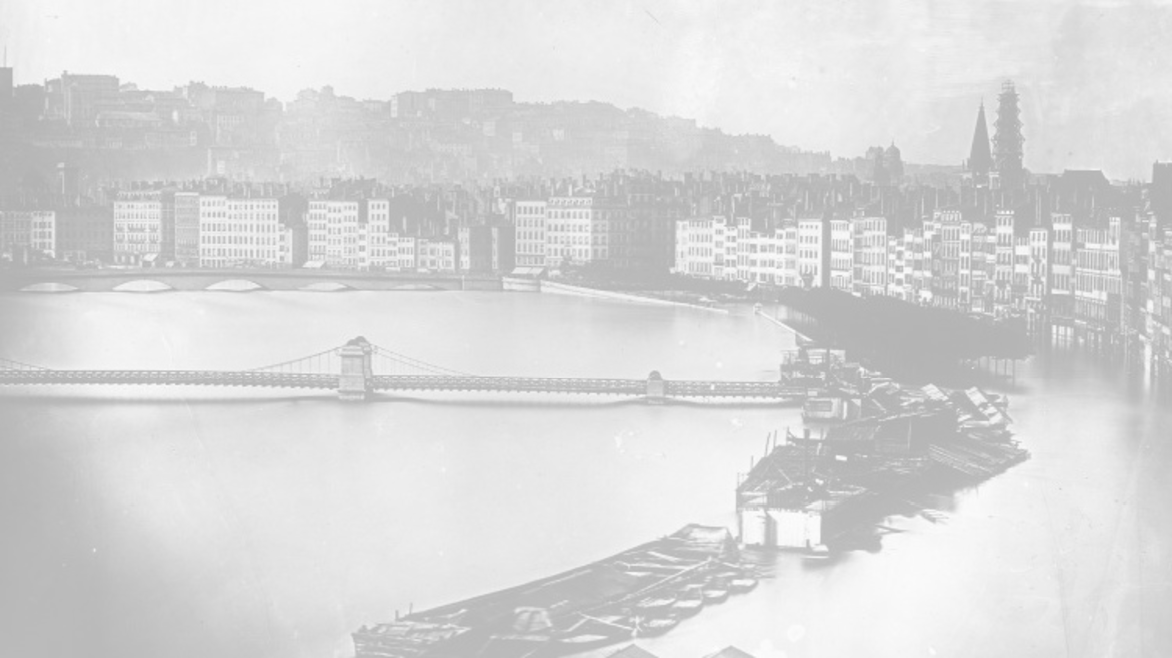
\includegraphics[height=\paperheight,width=\paperwidth]{./Figures/Back.pdf}}

\begin{frame}[plain]
     \vspace{10pt}
%     \vfill
     
\includegraphics[height= .5cm]{./Figures/CNR.png}	\hspace{4pt}
     
\includegraphics[height= .6cm]{./Figures/h2o.png}  \hspace{4pt}
     
\includegraphics[height= .5cm]{./Figures/INRAE.jpg}  \hspace{4pt}
     
\includegraphics[height= .6cm]{./Figures/lyon1.png}  \hspace{4pt}
     
\includegraphics[height= .6cm]{./Figures/MEGA.png}  \hspace{4pt} 
     
\includegraphics[height= .6cm]{./Figures/OSR.jpg}  \hspace{4pt}
     
\includegraphics[height= .6cm]{./Figures/Eu.jpg}  
     \centering
%     \begin{beamercolorbox}[sep=10pt,center,colsep=-4bp,rounded=true,shadow=true]{institute}
%     \end{beamercolorbox}
	\vspace{20pt}
     {\usebeamercolor[fg]{titlegraphic}\inserttitlegraphic\par}
     \begin{beamercolorbox}[sep=10pt,center,colsep=-4bp,rounded=true,shadow=true]{title}
        \usebeamerfont{title}\inserttitle\par%
%        \ifx\insertsubtitle\@empty%
%        \else%
%        \vskip0.25em%
%        {\usebeamerfont{subtitle}\usebeamercolor[fg]{subtitle}\insertsubtitle\par}%
%      \fi%     
     \end{beamercolorbox}%
     \vskip1em\par
     \begin{beamercolorbox}[sep=10pt,center,colsep=-4bp,rounded=true,shadow=true]{author}
%        \usebeamerfont{author}
        \Large{\insertauthor}
     \end{beamercolorbox}
%    \begin{beamercolorbox}[sep=5pt,center,colsep=-4bp,rounded=true,shadow=true]{author}
%    \centerize
    3 juillet 2023
   
  \flushleft \noindent \footnotesize Devant le jury composé de :\\
%\vspace{\stretch{1}}
%\begin{adjustwidth}{-0.8cm}{}
	\begin{center}
	\noindent \footnotesize{
	\begin{tabular}{llrl}
	    	\textsc{Carreau} & Julie & Professeure adjointe, Université de Montréal & Rapporteure\\
	    	\textsc{Llasat} & Maria-Carmen & Professeure, Université de Barcelone & Rapporteure\\
	    	\textsc{Favre}	& Anne-Catherine & Professeure, Université Grenoble Alpes & Examinatrice\\
	      	\textsc{Payrastre} & Olivier & IDTPE, Université Gustave Eiffel & Examinateur\\
	      	\textsc{Riviere} & Nicolas & Professeur, INSA Lyon & Examinateur\\
	      	\textsc{Ribereau} & Pierre & Maître de Conférences,  Université Lyon 1 & Examinateur\\
	      	\textsc{Lang} & Michel & ITPEHC , INRAE Villeurbanne & Directeur de thèse \\
	      	\textsc{Le Coz} & Jérôme & ICPEF, INRAE Villeurbanne & Co-encadrant\\
	      	\textsc{Renard} & Benjamin& Chargé de Recherche, INRAE Aix-en-Provence& Co-encadrant\\
	      	\textsc{Pierrefeu} & Gilles & Ingénieur, CNR & Invité \\
	\end{tabular}
	}
	\end{center}

%    \end{beamercolorbox}
%     \begin{beamercolorbox}[sep=8pt,center,colsep=-4bp,rounded=true,shadow=true]{date}
%        \usebeamerfont{date}\insertdate
%     \end{beamercolorbox}\vskip0.5em


\end{frame} 
}
\setcounter{page}{1}
\section{Introduction}
	\subsection{Le risque de crue}
	
	%%%%%%%%% 1 %%%%%%%%%
	\begin{frame}[c]
		\frametitle{Le risque d'inondation}
      	\begin{minipage}{0.39\textwidth}
      		\begin{itemize}
      			\item<1->[$\vartriangleright$] Type de catastrophe naturelle le plus fréquent dans le monde au XXI\textsuperscript{ème} siècle\footfullcite{UNDRR (2020). The human cost of disasters}
      			\vfill
      			\item<2->[$\vartriangleright$] Plus de 100 000 morts de 2000 à 2019
      			\vfill
      			\item<3->[$\vartriangleright$] 650 milliards de \$ de pertes économiques
      		\end{itemize}
      	\end{minipage}
      	\begin{minipage}{0.6\textwidth}
      		\begin{center}
      			\item \includegraphics<1>[width= .9\textwidth]{./Figures/1-Crue2005TyrolBBA-Imst.jpg}  
				\item \includegraphics<2->[width= .9\textwidth]{./Figures/2-UNDRR.png}  
      		\end{center}
      	\end{minipage}
	\end{frame}
		
%	\subsection{L'estimation du risque}
	
	%%%%%%%%% 2 %%%%%%%%%
	\begin{frame}%[c]
		\frametitle{L'estimation du risque}
		Nécessité de caractériser statistiquement l'aléa de crue :\\
    		\vspace{10pt}
      	\begin{minipage}{0.4\textwidth}  		
      		\begin{itemize}
      			\item<2->[$\vartriangleright$] PPRI
      			 $\Rightarrow$ \og\textit{événement le plus important connu ou} [...] \textit{évènement théorique de \textbf{fréquence centennale}, si ce dernier est plus important}\fg{} \footfullcite{Code de l'environnement (France); article R562-11-3}
      			\vspace{10pt}
      			\item<4>[$\vartriangleright$] Dimensionnement d'infrastructures à risque \\
      			$\Rightarrow$ \textbf{périodes de retour jusqu'à 10~000 ans}
      		\end{itemize}	
      	\end{minipage}
      	\begin{minipage}{0.59\textwidth}
      		\begin{center}
      		    \includegraphics<2>[width = .9\textwidth]{./Figures/3-PPRI_lyon0.pdf}
				\includegraphics<3>[width = .9\textwidth]{./Figures/4-PPRI_lyon.pdf}  
				\includegraphics<4>[width = .9\textwidth]{./Figures/5-Grangent.jpg} 
      		\end{center}
      	\end{minipage}
	\end{frame}
	
	%%%%%%%%% 3 %%%%%%%%%    %crues = réalisations + concept de période de retour
	\begin{frame}%[c]
		\frametitle{L'estimation du risque}
		Il est possible de modéliser les crues de façon probabiliste\\
      	\vfill
		\begin{center}
			\includegraphics[width = .8\textwidth]{./Figures/6-Réalisations.pdf} 
		\end{center}
		\vfill
		\begin{itemize}
			\item<2->[$\vartriangleright$] Les observations de crues $(x_1,...,x_n)$ sont des réalisations d'une variable aléatoire $X$ 
			\item<3->[$\vartriangleright$] \textbf{La théorie des valeurs extrêmes} nous donne le cadre pour modéliser ces processus \footfullcite{fisher_limiting_1928}\textsuperscript{;}\footfullcite{gumbel_statistics_1958} : loi généralisée des valeurs extrêmes ou $GEV(\mu,\sigma,\xi)$
		\end{itemize}
	\end{frame}
	
	\subsection{Analyse fréquentielle}
	
	
	%%%%%%%%% 5 %%%%%%%%%
	\begin{frame}%[c]
		\frametitle{Analyse fréquentielle des crues}
		\vfill
		Débit maximum annuel de \textbf{période de retour} T \\ $\Rightarrow$ probabilité $p = 1/T$ d'être \textbf{dépassé} chaque année
		\vfill
		\begin{center}
			\includegraphics<1>[width = .7\textwidth]{./Figures/Qamax.pdf} 
			\includegraphics<2>[width = .7\textwidth]{./Figures/Qamax_GEV.pdf} 
			\includegraphics<3>[width = .7\textwidth]{./Figures/Qamax_GEV_Q100.pdf} 
		\end{center}
	\end{frame}
	
	
	%%%%%%%%% 7 %%%%%%%%%
	\begin{frame}%[c]
		\frametitle{Analyse fréquentielle et incertitudes}
		Ces estimations affectées par des incertitudes :
		\vfill
      	\begin{itemize}
      		\item<2->[$\vartriangleright$] \textbf{Hypothèses de modélisation} : choix d'une distribution, stationnarité...
      		\vspace{5pt}
      		\item<3->[$\vartriangleright$] \textbf{Hydrométrie} : estimation du débit des cours d'eau
      		\vspace{5pt}
      		\item<4->[$\vartriangleright$] \textbf{Échantillonnage} : longueur limitée des échantillons de crues
      	\end{itemize}
      	\vfill
      	\onslide<5-> Leur détermination est \textbf{essentielle} pour :
      	\vfill
      	\begin{itemize}
      		\item<6->[$\vartriangleright$] aider à la prise de décision 
      		\vspace{5pt}
      		\item<7->[$\vartriangleright$] comprendre l'apport des informations historiques
      	\end{itemize}
	\end{frame}
	
	\subsection{Incertitude hydrométrique}
	%%%%%%%%% 8 %%%%%%%%%
	\begin{frame}[t]
		\frametitle{Incertitudes hydrométriques}
      	Le débit des cours d'eau ne peut être mesuré en continu
		\vfill
		\begin{center}
			\includegraphics<2>[width = .6\textwidth]{./Figures/LimniVienne.png}
			\includegraphics<3>[width = .7\textwidth]{./Figures/Hydrom1.pdf}
			\includegraphics<4>[width = .7\textwidth]{./Figures/Hydrom2.pdf}
			\includegraphics<5>[width = .7\textwidth]{./Figures/Hydrom3.pdf}
			\includegraphics<6>[width = .7\textwidth]{./Figures/Hydrom4.pdf}
		\end{center}

	\end{frame}
	
	%%%%%%%%% 9 %%%%%%%%%
	\begin{frame}%[c]
		\frametitle{Incertitudes hydrométriques}
		\begin{center}\begin{itemize}
		\centering
			\item<1->[\Huge{$\textcolor{green}{\checkmark}$}] Méthodes de calcul des incertitudes à chaque étape\\
			\vspace{10pt}
			\item<2>[\Huge{$\textcolor{red}{X}$}] Propagation complète et homogène des incertitudes
		\end{itemize}\end{center}	
		\vspace{10pt}
		\begin{center}
			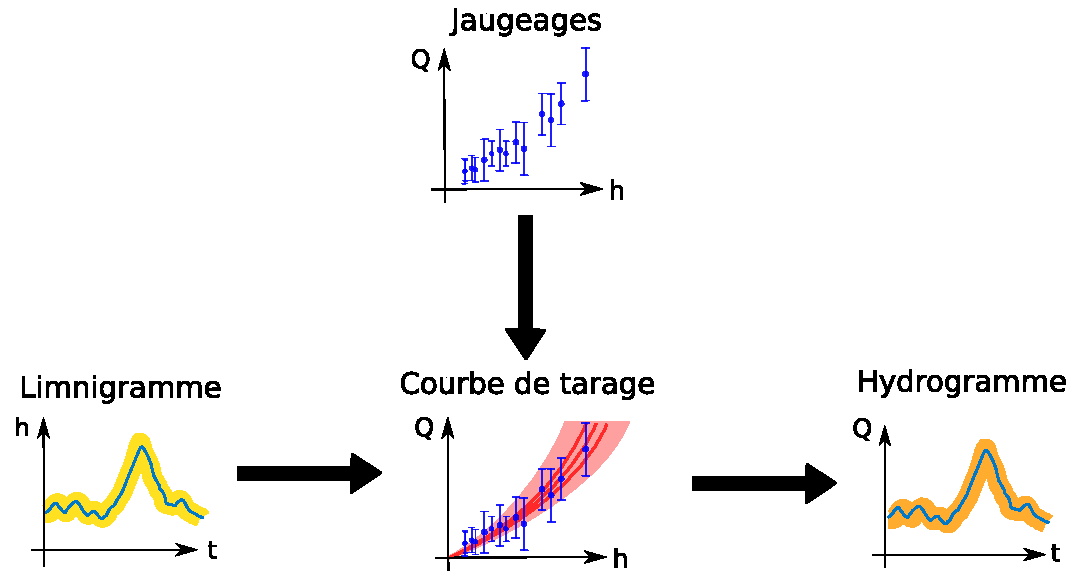
\includegraphics[width = .7\textwidth]{./Figures/Hydrom4.pdf}
		\end{center}
	\end{frame}
	
	%% Q1 %%
	\begin{frame}
		\frametitle{Incertitudes hydrométriques}
		\centering
		\vfill
%		\begin{beamercolorbox}[sep=10pt,center,colsep=-4bp,rounded=true,shadow=true]{
		\Large{\textbf{Q.1 : Comment estimer et propager de façon homogène l'ensemble des incertitudes hydrométriques ?}}
		%}
		%\end{beamercolorbox}
		\vfill
	\end{frame}
	
    	%%%%%%%%% X %%%%%%%%%
	\begin{frame}%[c]
		\frametitle{Incertitudes hydrométriques}
		\begin{center}
			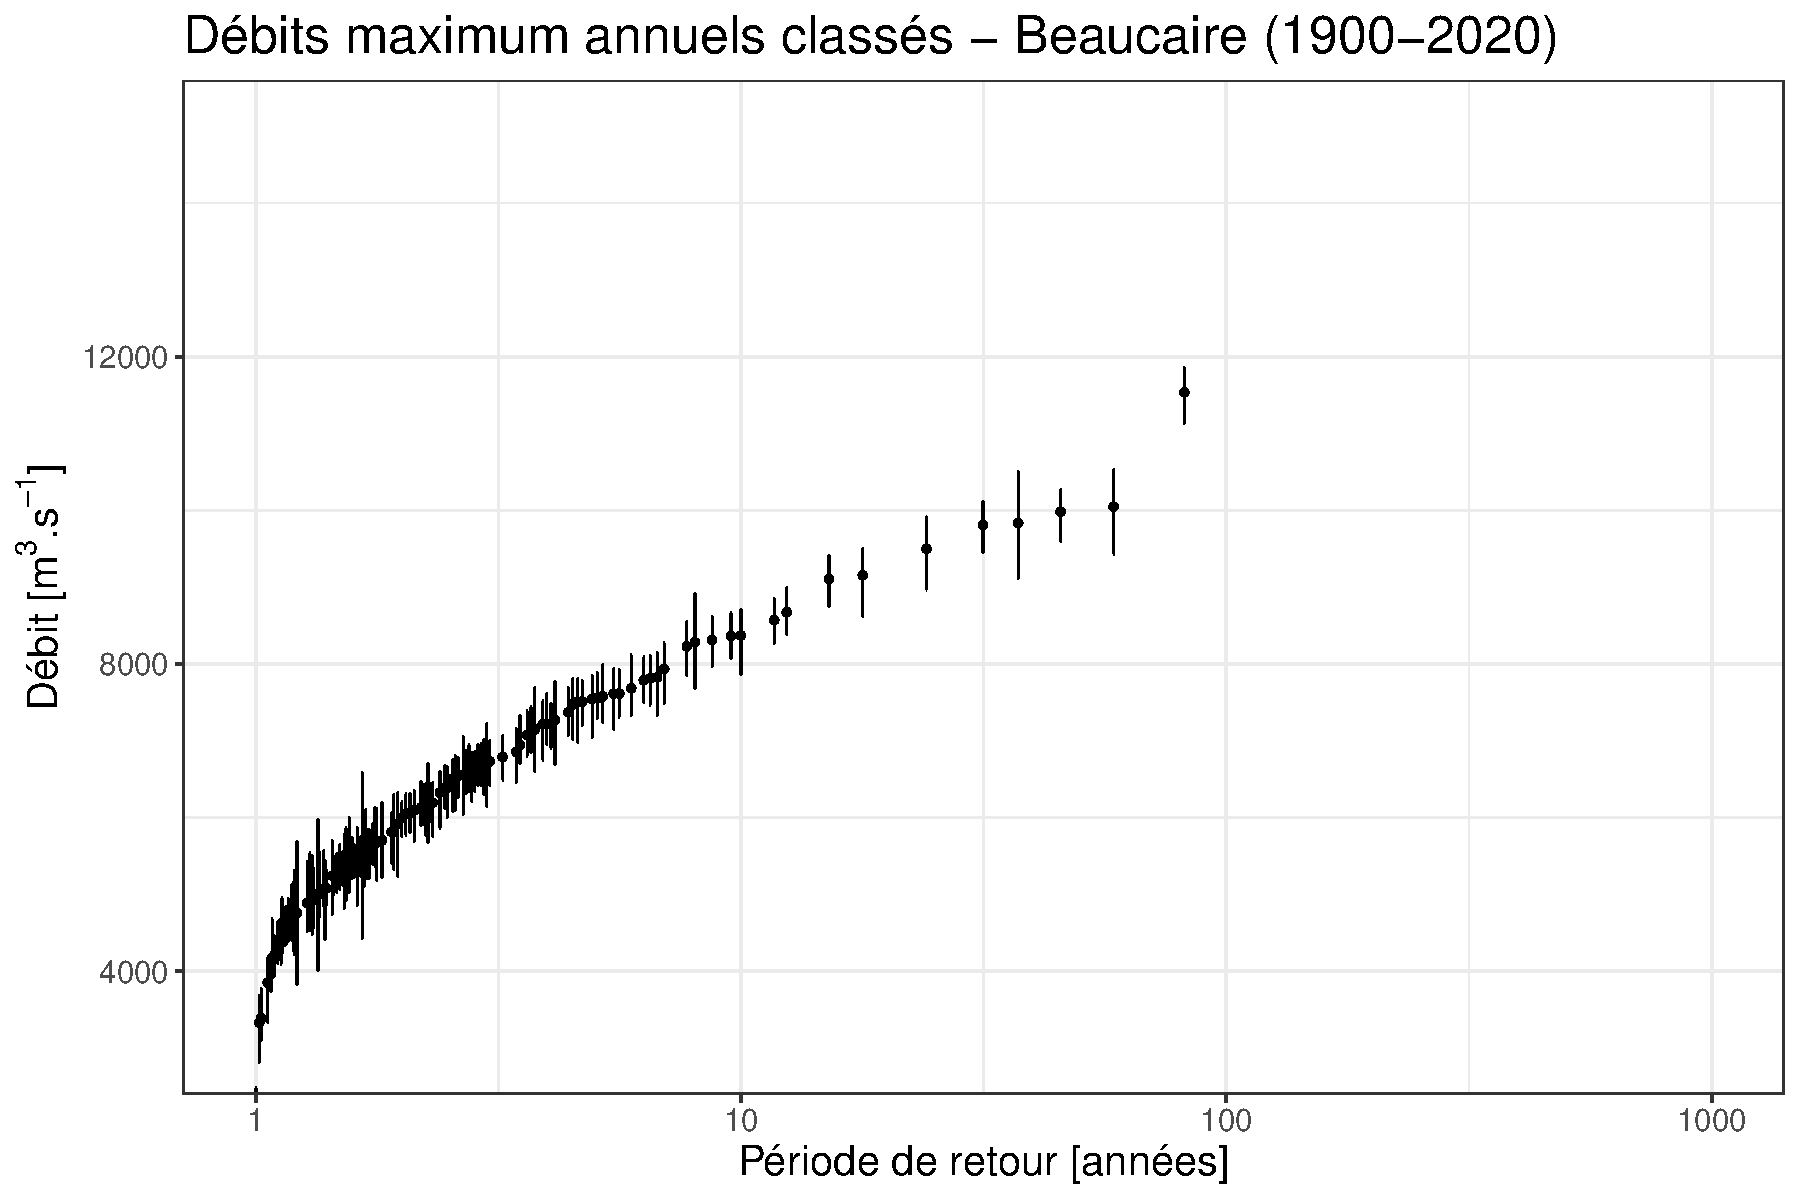
\includegraphics[width = .8\textwidth]{./Figures/Qamax_uQ.pdf} 
		\end{center}
	\end{frame}
	
	\subsection{Incertitude d'échantillonnage}    
    %%%%%%%%% 12 %%%%%%%%%
	\begin{frame}[t]
		\frametitle{Incertitude d'échantillonnage}
      	\begin{itemize}
			\item<1->[$\vartriangleright$] Longueur des chroniques de débit limitée $\Rightarrow$ 60 ans en moyenne en France\footfullcite{le_coz_quantifying_2017}
			\vspace{2pt}
			\item<2->[$\vartriangleright$] Périodes de retour ciblées plus grandes : 100, 1000, 10 000 ans
		\end{itemize}
		\vfill
      	\begin{center}
%      		\includegraphics<1>[width = .25\textwidth]{./Figures/LogoSampling.pdf}
%      		\includegraphics<2-3>[width = .6\textwidth]{./Figures/NbStationsHydro.pdf}
			\includegraphics<3>[width = .6\textwidth]{./Figures/Qsample1.pdf}
			\includegraphics<4->[width = .6\textwidth]{./Figures/Qsample2.pdf}\phantom{s}\\
			\vfill
			\centering
			\onslide<5-> Il est possible\footfullcite{coles_classical_2001} et nécessaire d'\textbf{estimer cette incertitude} 	
		\end{center}
	\end{frame}
		
		\begin{frame}
		\frametitle{Chaine de propagation des incertitudes}
		\begin{minipage}{0.45\textwidth}
%		\begin{center} \textbf{Relevés systématiques de hauteurs d'eau anciennes} \end{center}
			\begin{itemize}
				\vfill
				\item [$\vartriangleright$] Estimation et propagation successive des deux sources d'incertitude\\
%				\vspace{15pt}				
%				\item [$\vartriangleright$] Propagation successive des deux sources d'incertitude\\
%				\vspace{15pt}		
%				\item [$\vartriangleright$] Réduction de l'incertitude des quantiles en utilisant des relevés anciens ? \\
			\end{itemize}
			\vfill
		\end{minipage}
		\hfill		
		\begin{minipage}{0.53\textwidth}
			\centering
			\vfill
			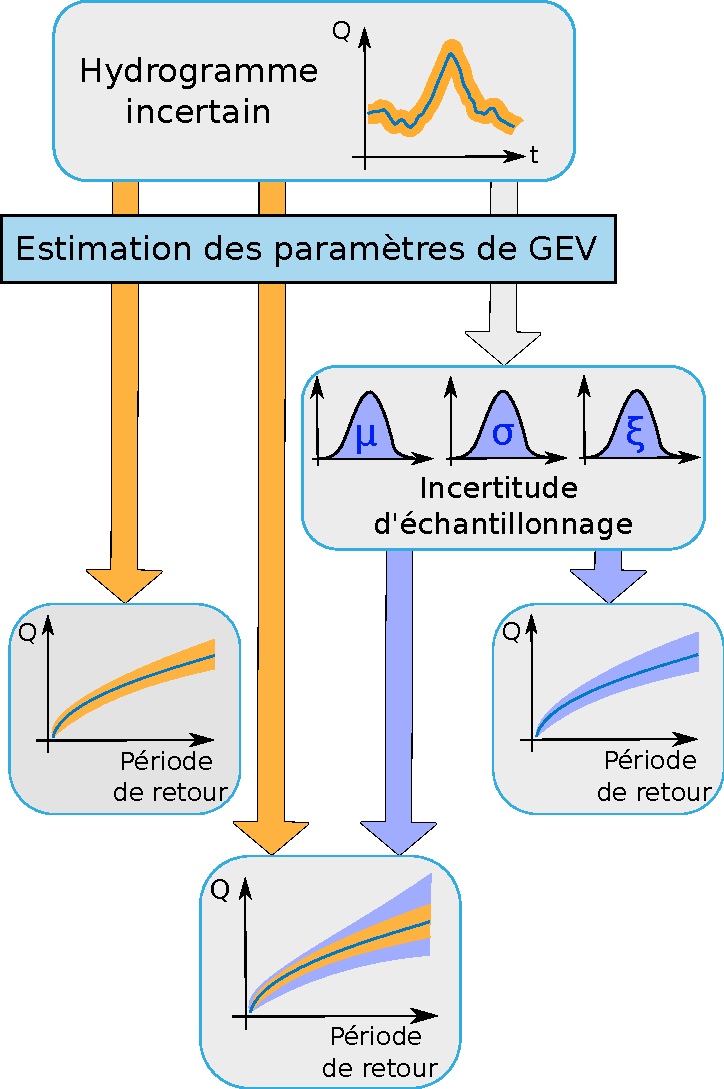
\includegraphics[width = .55\textwidth]{./Figures/uPropagtot.pdf}
		\end{minipage}
	\end{frame}
	                
	\begin{frame}
		\frametitle{Part respective des différentes incertitudes}
		\centering
		\vfill
%		\begin{beamercolorbox}[sep=10pt,center,colsep=-4bp,rounded=true,shadow=true]{
		\Large{\textbf{Q.2 :\\
		\vfill
		Comment estimer la part respective de l'incertitude hydrométrique et de l'incertitude d'échantillonnage dans l'incertitude totale des quantiles ? \\
		\vfill
		Jusqu'à quelle limite l'utilisation de limnigrammes anciens permet de réduire l'incertitude des quantiles ?} }%}
		%\end{beamercolorbox}
		\vfill
	\end{frame}
	
	
	\subsection{Crues historiques}    
	%%%%%%%%% X %%%%%%%%%
	\begin{frame}[c]
		\frametitle{Incertitude d'échantillonnage}
		\vspace{5pt}
		Élargir le jeu de données $\Rightarrow$ Diminuer l'incertitude d'échantillonnage\\
		\vspace{10pt}
		\begin{minipage}[t]{0.49\textwidth}
			\begin{itemize}
				\centering
				\item<2->[$\vartriangleright$] \textbf{Spatialement}
			\end{itemize}
			\vspace{2pt}
			\centering
			\includegraphics<2->[width = .6\textwidth]{./Figures/Regional.pdf}\phantom{s}\\
			\vspace{2pt}
			\onslide<2->\scriptsize{Bassins versants méditerranéens\footfullcite{gaume_bayesian_2010}} \\
			\vspace{2pt}
%			\onslide<3-> \normalsize{Homogénéité régionale}
		\end{minipage}
		\begin{minipage}[t]{0.49\textwidth}
			\begin{itemize}
				\centering
				\item<3->[$\vartriangleright$] \textbf{Temporellement}
			\end{itemize}
			\vspace{7pt}
			\centering
			\includegraphics<3>[width = .9\textwidth]{./Figures/HistoFloods1.pdf}%\phantom{s}\\
			\includegraphics<4>[width = .9\textwidth]{./Figures/HistoFloodsAll.pdf}%\phantom{s}\\
			\includegraphics<5>[width = .85\textwidth]{./Figures/HistoFloodsRed.pdf}\phantom{s}\\
			\vspace{1pt}
			\onslide<3-> \scriptsize{Red River of the North à Winnipeg, Canada \footfullcite{st_george_paleofloods_2020}} \\
			\vspace{2pt}
%			\onslide<6-> \normalsize{Homogénéité temporelle}
		\end{minipage}
	\end{frame}
	
	%%%%%%%%% X %%%%%%%%%
	\begin{frame}[t]
		\frametitle{Crues historiques et analyse fréquentielle}
		\centering
		Les données de crues historiques peuvent prendre des formes diverses :
		\vfill
		\begin{minipage}{0.49\textwidth}
	      	\begin{itemize}
	      		\item<2->[$\vartriangleright$] Relevés systématiques non-bancarisés \footfullcite{pichard_les_1995}\textsuperscript{;}\footfullcite{bard_actualisation_2018}
	      		\item<3->[$\vartriangleright$] Repères de crue\footfullcite{parkes_defining_2016}\textsuperscript{;}\footfullcite{engeland_new_2020}\textsuperscript{;}\footfullcite{renard_use_2023}
	      		\item<4->[$\vartriangleright$] Témoignages\footfullcite{pichard_les_1995}\textsuperscript{;}\footfullcite{neppel_flood_2010} 
	      		\item<5->[$\vartriangleright$] Reconstructions issues de divers proxys \footfullcite{dezileau_multidating_2014}\textsuperscript{;}\footfullcite{wilhelm_reconstructing_2022}% \textsuperscript{;}\footfullcite{ballesteros-canovas_review_2015}
	      	\end{itemize}
      	\end{minipage}
      	\hfill
      	\begin{minipage}{.45\textwidth}
      		\begin{center}
      		\includegraphics<2>[width = .8\textwidth]{./Figures/TabObs.jpg} 
      		\includegraphics<3>[width = .4\textwidth]{./Figures/RepAvi.jpg} 
      		\includegraphics<4>[width = .75\textwidth]{./Figures/Parchemin.jpg} 
      		\includegraphics<5>[width = .35\textwidth]{./Figures/Sedim.pdf} 
      		\includegraphics<6->[width = .7\textwidth]{./Figures/Dendro.jpg} \phantom{s}\\
			\end{center}
      	\end{minipage}
      	\vfill
      	\centering
      	\onslide<7> Données généralement \textbf{sporadiques} $\Rightarrow$ nécessitent des \textbf{traitements statistiques adaptés}
%      	\onslide<7-> Prise en compte complète et homogène des incertitudes \textbf{généralement oubliée}
	\end{frame}
	

	
	\begin{frame}[t]
		\frametitle{Concept de seuil de perception}
		\vfill
		\begin{center}
			Données de crues historiques : \textbf{sporadiques} $\Rightarrow$ exhaustivité ?\\
			\vspace{5pt}
			Concept de \textbf{seuil de perception} \footfullcite{gerard_probability_1979}\textsuperscript{;}\footfullcite{stedinger_flood_1986}\\
		\end{center}
		\vfill
		\begin{itemize}
			\item<2-> [$\vartriangleright$] Années avec mentions de crue historique $\Rightarrow$ Débit > Seuil de perception 
			\vspace{10pt}
			\item<3-> [$\vartriangleright$] Années sans mentions de crue $\Rightarrow$ Débit < Seuil de perception
%			\vspace{10pt}
%			\item<4-> [$\vartriangleright$] Connaissance du débit des crues historiques pas obligatoire : \textbf{nombre de dépassements} du seuil suffisant \textsuperscript{19;}\footfullcite{payrastre_usefulness_2011}
		\end{itemize}
		\vfill
	\end{frame}
	
	\begin{frame}
		\frametitle{Témoignages historiques et incertitudes}
		Seuil de perception $\boldsymbol{S}$ généralement considéré comme étant \textbf{parfaitement connu}\\
%		\begin{center} $\Rightarrow$ \Large{optimisme ?}\\ \end{center}
		\vspace{10pt}
		\begin{itemize}
		\item [$\vartriangleright$]Tests de sensibilité \footfullcite{stedinger_flood_1986}\textsuperscript{;}\footfullcite{macdonald_reassessing_2014}\textsuperscript{;}\footfullcite{payrastre_usefulness_2011}\textsuperscript{;}\footfullcite{parkes_defining_2016} mais pas d'estimation de l'incertitude résultante
		\end{itemize}
		\vfill
		\onslide<2-> Durée de la période historique $\boldsymbol{n}$ considérée comme étant \textbf{parfaitement connue} %$\Rightarrow$ délicate à estimer
		\vspace{10pt}
		\begin{itemize}
		\item<2->[$\vartriangleright$] Méthode permettant d'en donner une estimation\footfullcite{prosdocimi_german_2018}, mais pas d'impact sur l'incertitude des quantiles de crue
		\end{itemize}
		\vfill
	\end{frame}
	
	\begin{frame}
		\frametitle{Données historiques et incertitudes}
		\centering
		\large{\textbf{Q.3 :\\
		\vfill
		Comment considérer une incertitude sur le seuil de perception et la durée de la période historique ?\\
		\vfill
		Quel est l'apport des témoignages de crues historiques pour l'analyse fréquentielle ?\\}}
		\vfill
		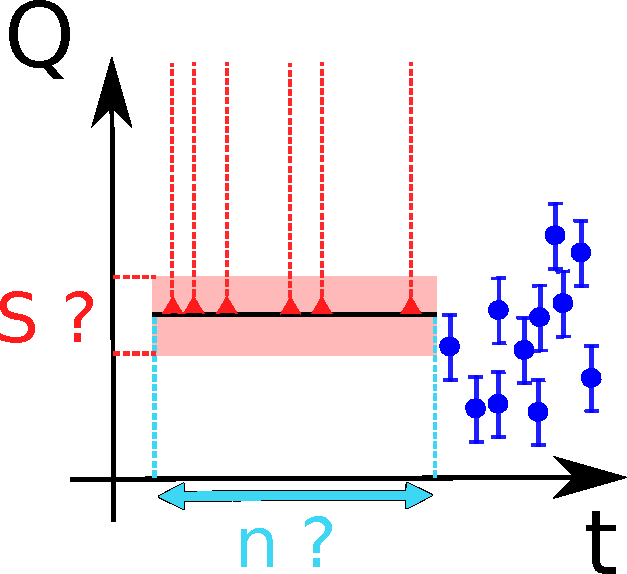
\includegraphics[width = .35\textwidth]{./Figures/uSuN.pdf}
	\end{frame}
	
	\subsection{Problématiques et objectifs}
	%%%%%%%%% X %%%%%%%%%	
	\begin{frame}
	    \frametitle{Problématiques}
		\vfill
		\large{\textbf{1-Estimation de l'incertitude hydrométrique}}
		\vspace{5pt}
		\begin{itemize}
			\item [$\vartriangleright$] Comment estimer et propager de façon homogène l'ensemble des incertitudes hydrométriques ? 
		\end{itemize}
		\vfill
		\onslide<2->\large{\textbf{2-Incertitude hydrométrique VS incertitude d'échantillonnage}}
		\vspace{5pt}
		\begin{itemize}
%			\item [$\vartriangleright$] Comment estimer la part respective de l'incertitude hydrométrique et de l'incertitude d'échantillonnage dans l'incertitude totale des quantiles ?\\
			\item<2->[$\vartriangleright$] Jusqu'à quelle limite l'utilisation de limnigrammes anciens permet de réduire l'incertitude des quantiles ?
		\end{itemize}
		\vfill
		\onslide<3->\large{\textbf{3-Analyse fréquentielle historique}}
		\vspace{5pt}
		\begin{itemize}
			\item<3-> [$\vartriangleright$] Comment considérer une incertitude sur le seuil de perception et la durée de la période historique ?\\
			\item<3->[$\vartriangleright$] Quel est l'apport des témoignages de crues historiques pour l'analyse fréquentielle ?
		\end{itemize}
		\vfill
	\end{frame}
	
	%%%%%%%%% X %%%%%%%%%	
%	\begin{frame}
%	    \frametitle{Objectifs de la thèse}
%	    \begin{itemize}
%	    \vfill
%	    \item<1->[$\vartriangleright$]  Estimer et propager de façon complète et homogène les différentes sources d'incertitudes hydrométriques jusqu'aux séries de débit
%	    \vfill
%	    \item<2->[$\vartriangleright$]  Estimer la part de ces deux incertitudes dans l'incertitude totale des quantiles de crue
%	    \vfill
%	    \item<3->[$\vartriangleright$]  Mettre au point un modèle qui considère une incertitude sur le seuil de perception et la durée des échantillons de crues historiques
%	    \vfill
%	    \item<4->[$\vartriangleright$] Quantifier l'apport de l'information historique lors de l'analyse fréquentielle
%	    \vfill
%	    \end{itemize}
%	\end{frame}
	
	
%\section{Cas d'étude}
	\subsection{Le Rhône à Beaucaire}
	{
    \setbeamercolor{background canvas}{bg=myblue}
    \begin{frame}
        \begin{center}
				\textcolor{white}{\Large \textbf{Cas d'étude : Le Rhône à Beaucaire}}\\
		 		\vspace{0.3cm}
		 		\textcolor{white}{\large \textbf{Collecte et caractérisation des données de crue}}\\
		 		\vspace{0.7cm}
		 		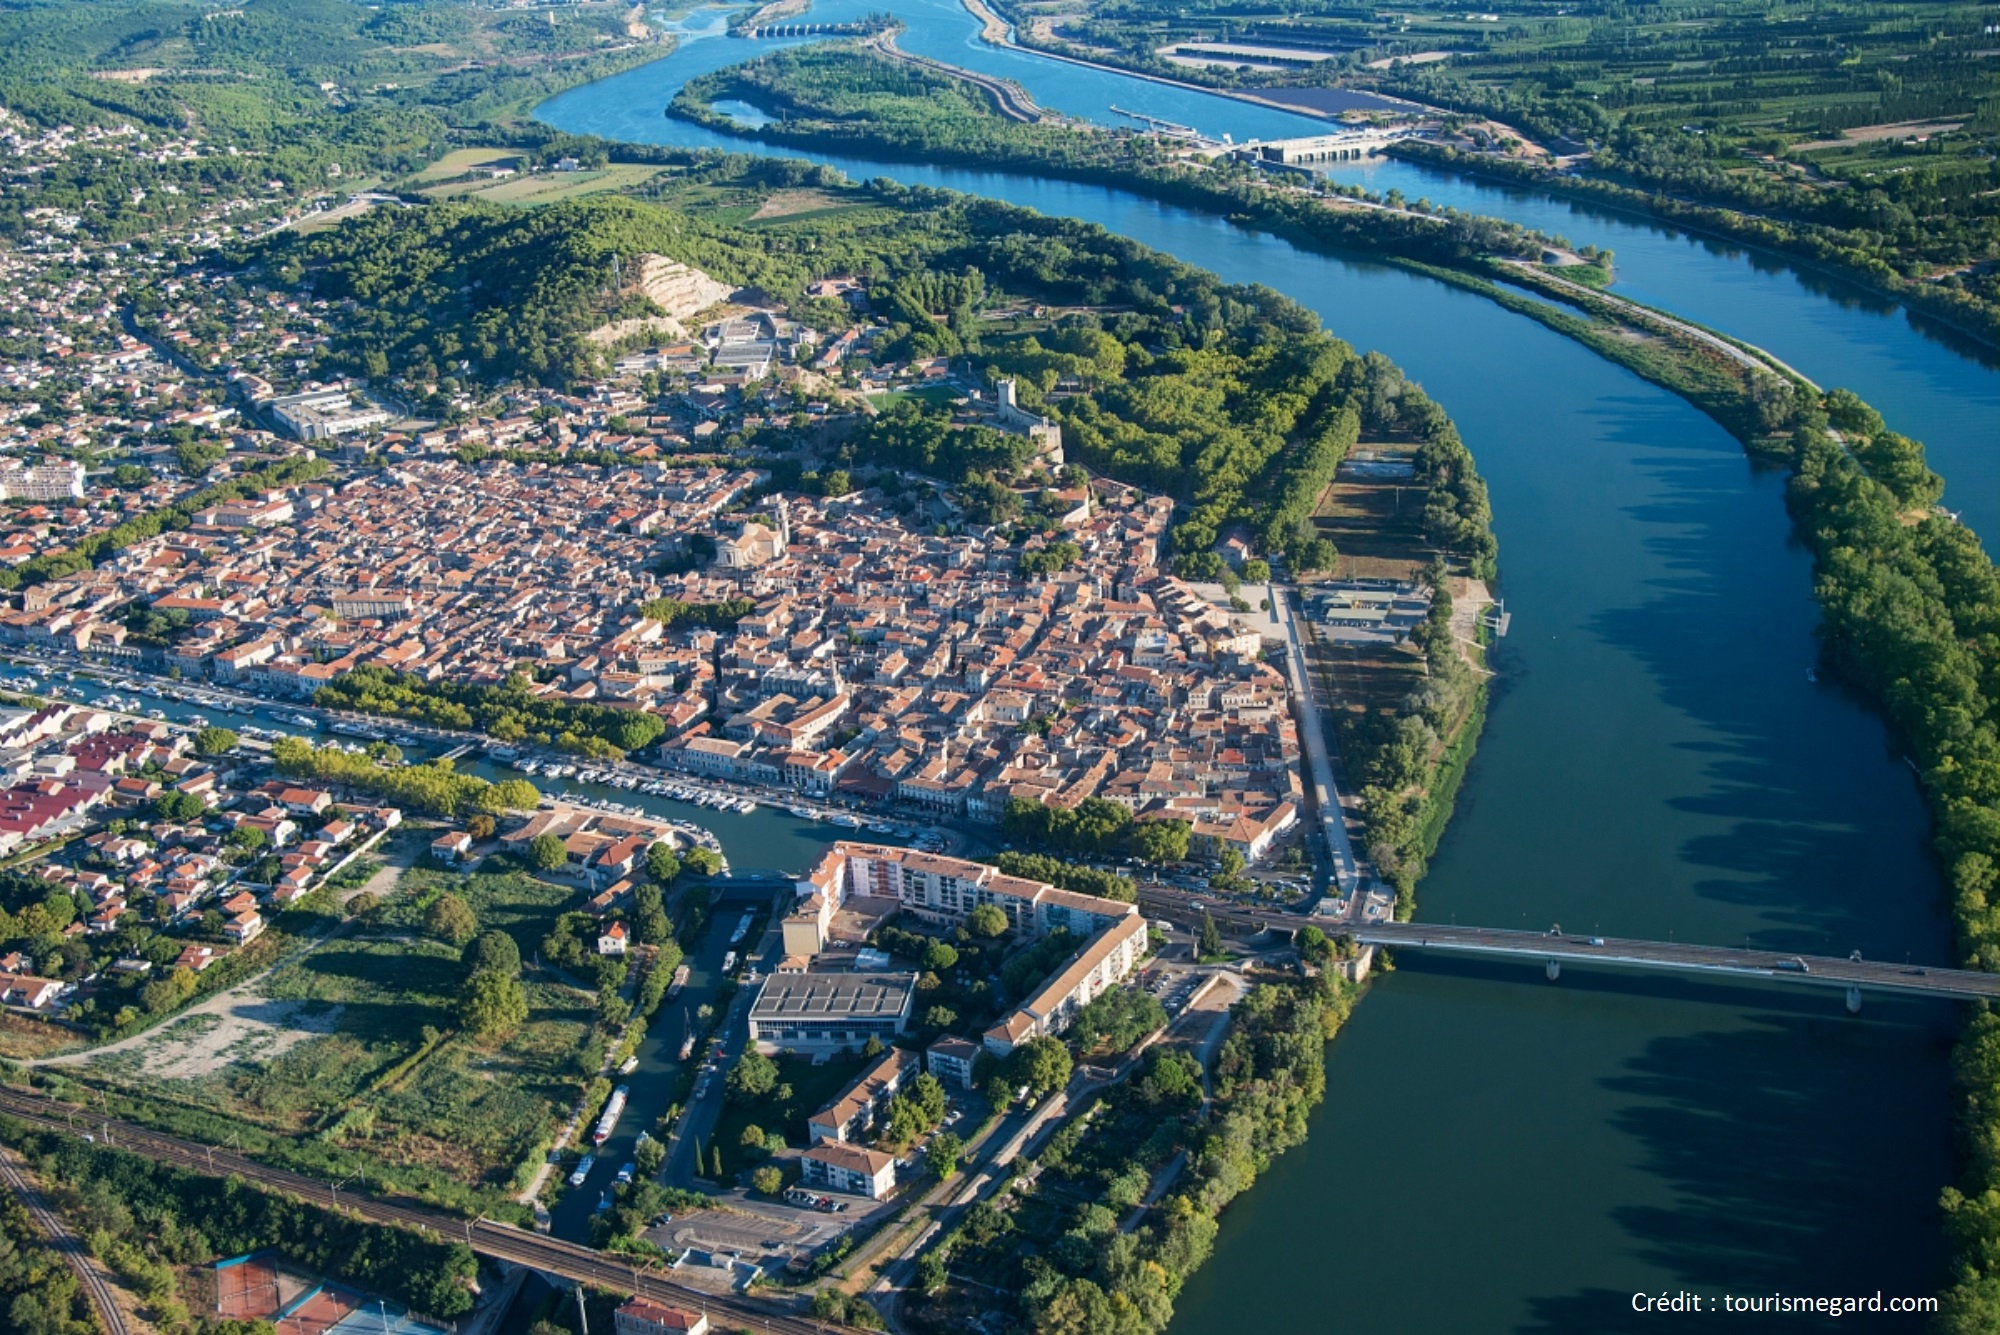
\includegraphics[width = .7\textwidth]{./Figures/BcrAerien.jpg} 
        \end{center}
    \end{frame}
    }
    	
    \subsection{Présentation}
	%%%%%%%%% 19 %%%%%%%%%
	\begin{frame}%[c]
		\frametitle{Le Rhône à Beaucaire}
		\begin{minipage}{.5\textwidth}
			\begin{itemize}
				\item<1->[$\vartriangleright$] Bassin versant de 95 590 km²\\
				\vfill
				\item<3->[$\vartriangleright$] Apports variés et complexes : \og\textit{il comporte une infinité de nuances et de contrastes}\fg{}   \footfullcite{parde_regime_1925}\\
				\vfill
				\item<4->[$\vartriangleright$] Dernière station du Rhône complet\\
			\end{itemize}
		\end{minipage}
		\hfill
		\begin{minipage}{.4\textwidth}
			\centering
	      	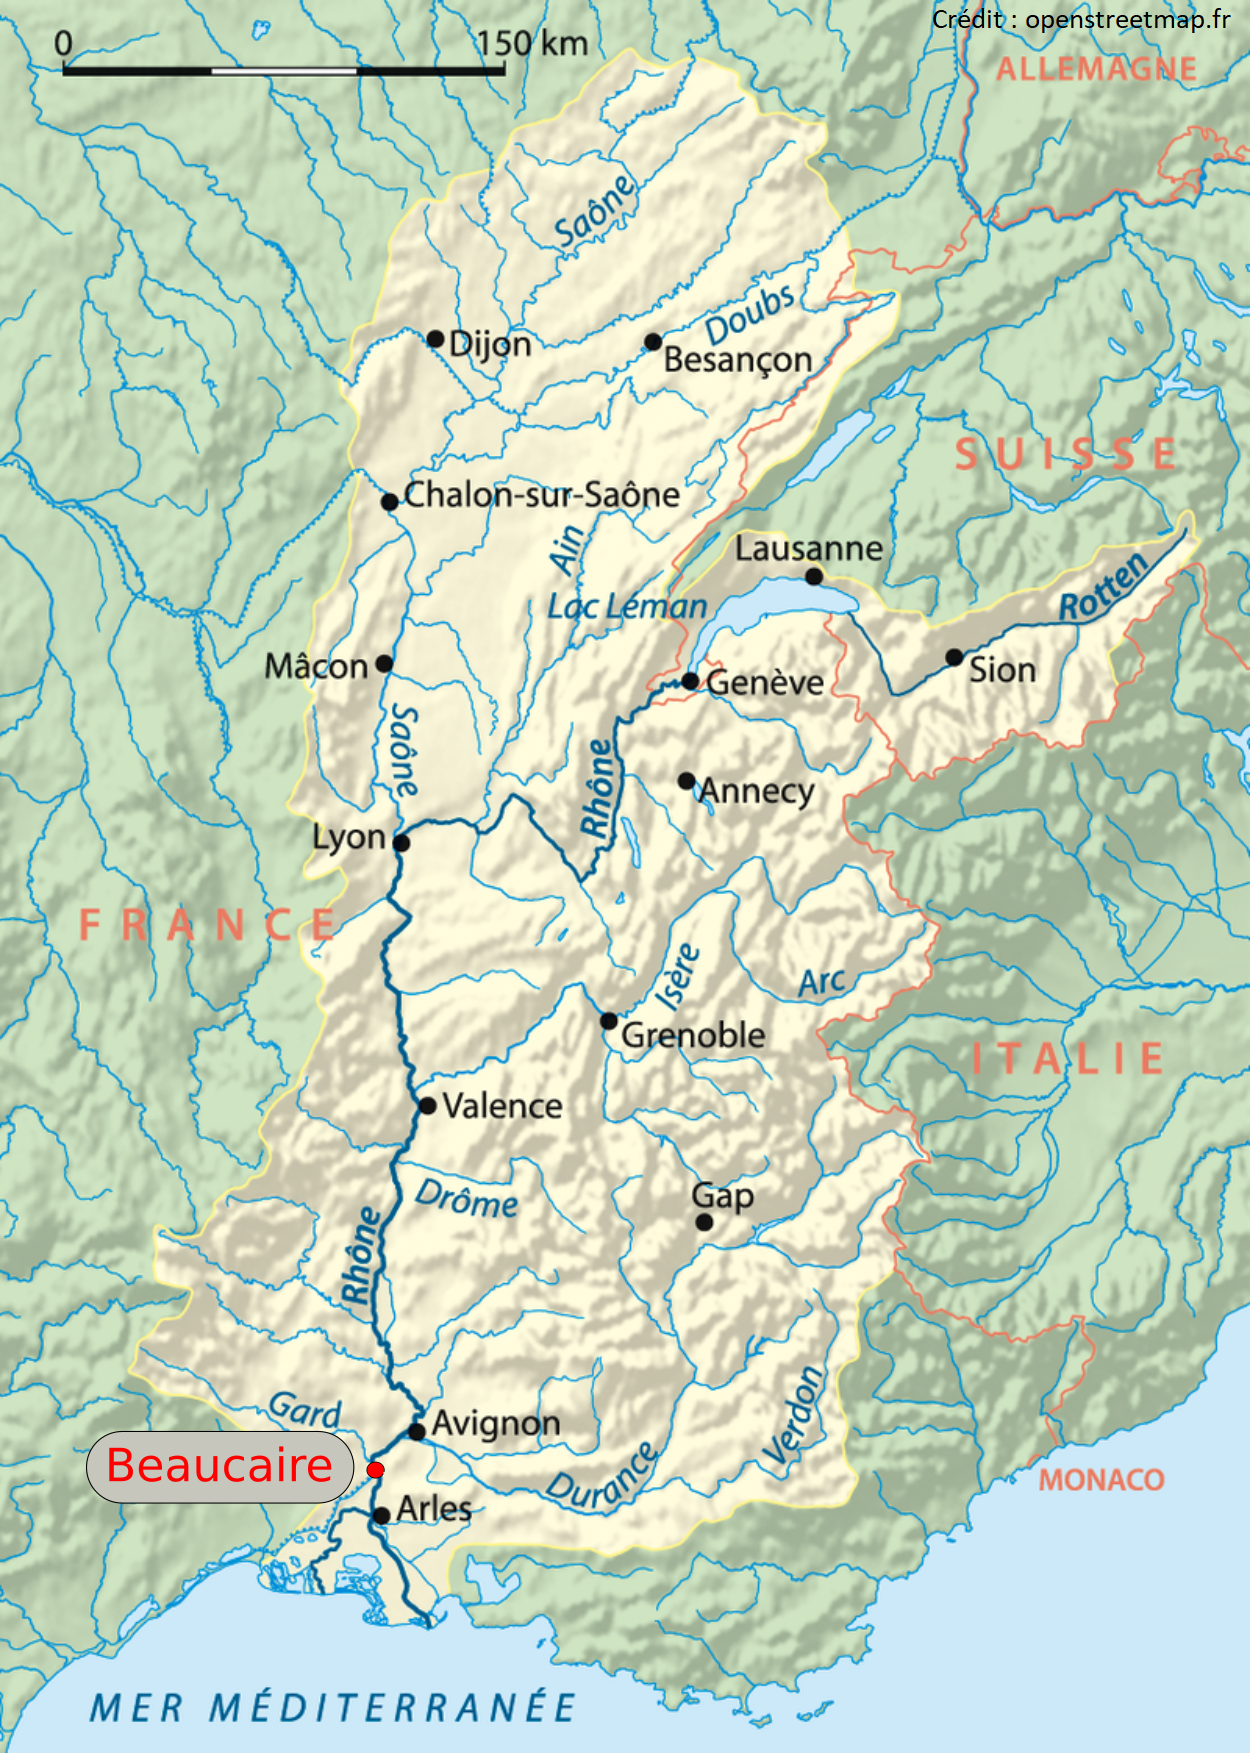
\includegraphics[width = \textwidth]{./Figures/Rhone_bassin_versant.png} 
		\end{minipage}
	\end{frame}
	
%	%%%%%%%%% 20 %%%%%%%%%
%	\begin{frame}%[c]
%		\frametitle{Régime hydrologique}
%		\centering
%      	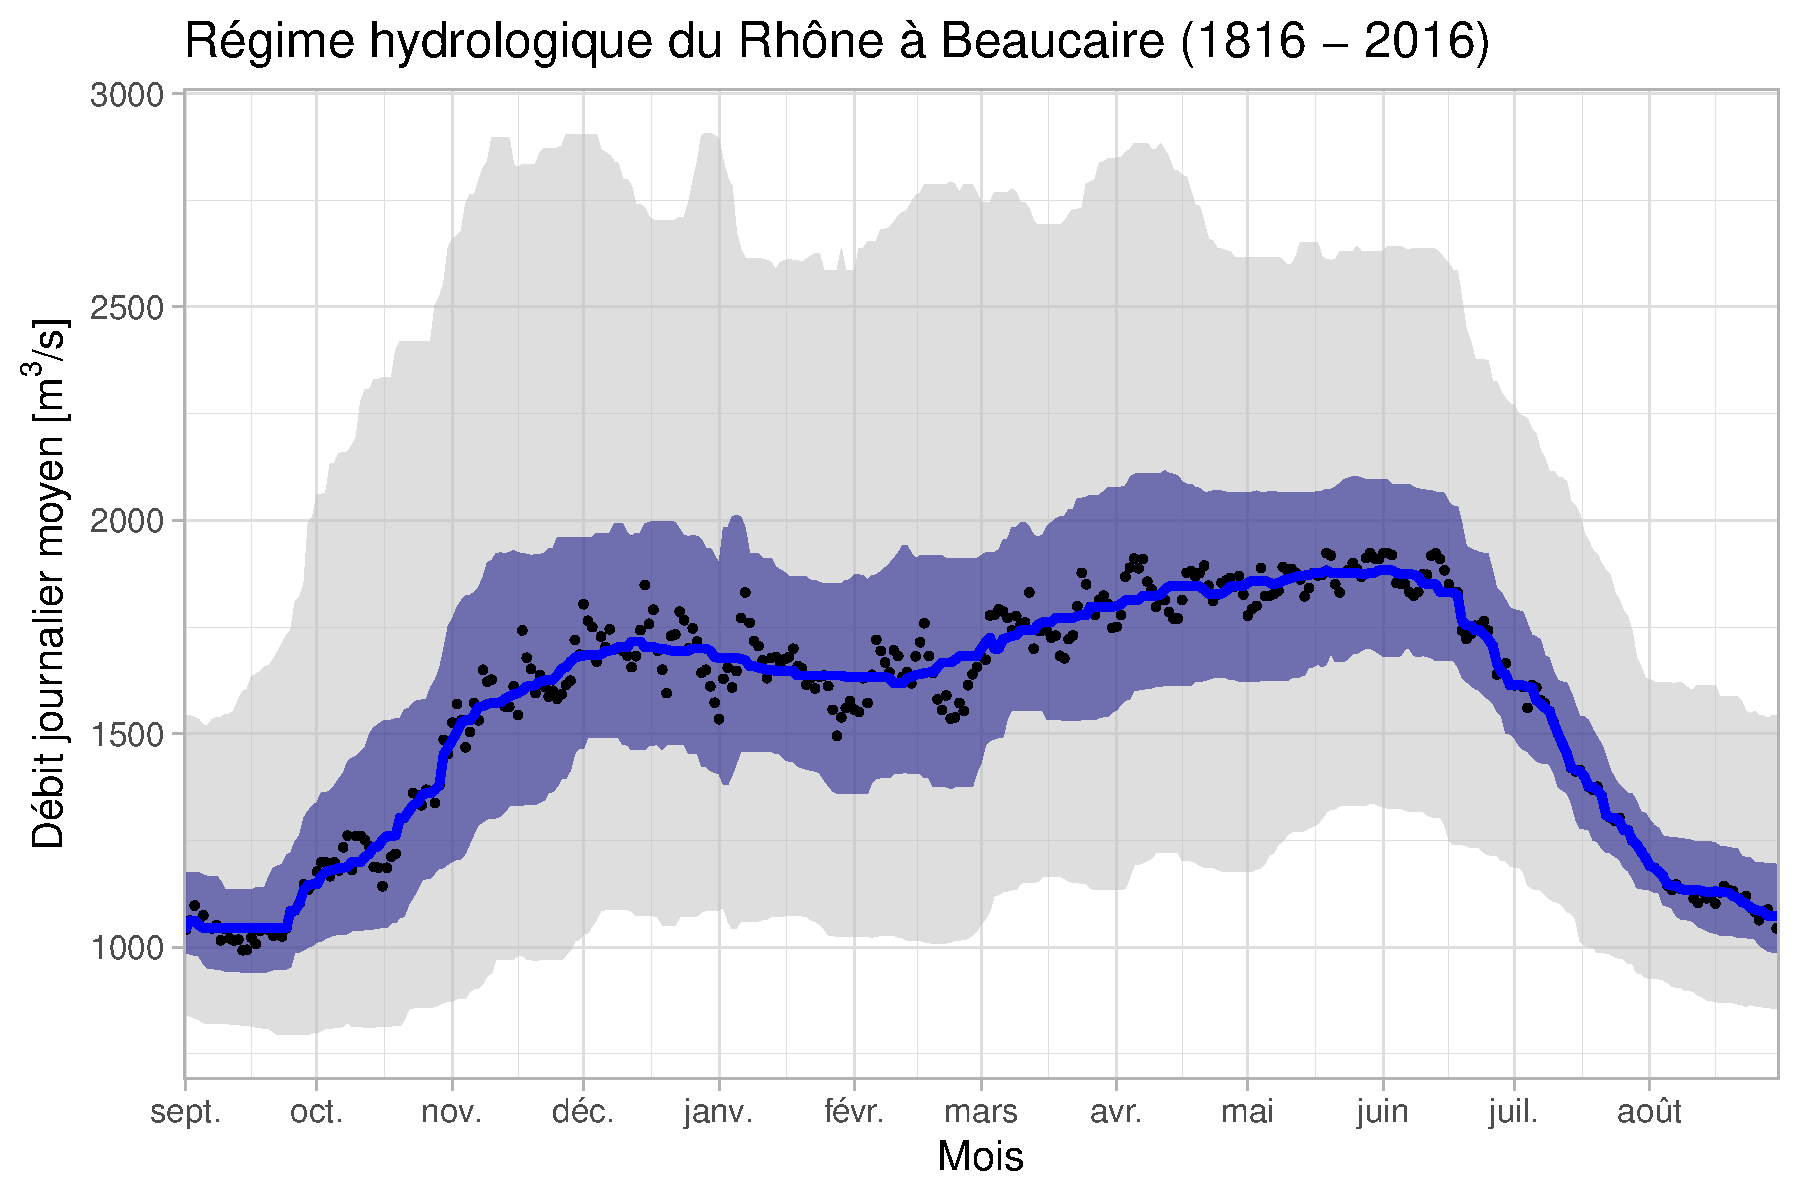
\includegraphics[width = .7\textwidth]{./Figures/Regime.pdf}\phantom{s}\\
%      	\centering     	
%      	Débits moyens journaliers et quantiles (20, 40, 60 et 80\%)
%	\end{frame}
%	
	%%%%%%%%% 21 %%%%%%%%%
	\begin{frame}%[c]
		\frametitle{Beaucaire et le Rhône}
		\begin{minipage}{.39\textwidth}
			\begin{itemize}
				\item<1->[$\vartriangleright$] Foire de Beaucaire : \og \textit{Capitale française des marchandises} \fg{}\footfullcite{leon_vie_1953}\\
				\vspace{15pt}
				\item<2->[$\vartriangleright$] Fortes crues au XIX\textsuperscript{ème} siècle et en 2003\\
				\vfill
			\end{itemize}
		\end{minipage}
		\begin{minipage}{.6\textwidth}
		\vfill
			\begin{center}
	      		\includegraphics<1>[width = \textwidth]{./Figures/foire5.jpg} 
	      		\includegraphics<2>[width = \columnwidth]{./Figures/Napo.jpg} 
	      		\includegraphics<3>[width = .9\textwidth]{./Figures/2003.jpg} 
%	      		\includegraphics<4>[width = .6\textwidth]{./Figures/StationBcr.jpg} 
			\end{center}
			\vfill
		\end{minipage}
	\end{frame}
	
	
	
	%%%%%%%%% 22 %%%%%%%%%
	\subsection{Station hydrométrique}
	\begin{frame}%[c]
		\frametitle{Station hydrométrique (1816-2020)}
		\begin{minipage}{.4\textwidth}
			\begin{itemize}
				\item<1->[$\vartriangleright$] Relevés quotidiens dès 1816 : "\textbf{Pont de Beaucaire}"\\
				\vfill
				\item<4->[$\vartriangleright$] Travaux CNR 1967-1970\\
				\vfill
				\item<5->[$\vartriangleright$] Déplacement 2 km à l'aval : "\textbf{Beaucaire Restitution}"\\
				\vfill
				\item<6>[$\vartriangleright$] Jaugeages dès 1845\\
			\end{itemize}
		\end{minipage}
		\hfill
		\begin{minipage}{.59\textwidth}
			\begin{center}
	      		\includegraphics<1>[width = \textwidth]{./Figures/Pt.jpg} 
	      		\includegraphics<2>[width = .5\textwidth]{./Figures/StationBCR.jpg} 
	      		\includegraphics<3>[width = .9\columnwidth]{./Figures/TabObs.jpg} 
	      		\includegraphics<4>[width = .9\columnwidth]{./Figures/Vallab.jpg} 
	      		\includegraphics<5>[width = .9\columnwidth]{./Figures/EchelleRestit.jpg} 
	      		\includegraphics<6>[width = \textwidth]{./Figures/Jaus.pdf}
			\end{center}
		\end{minipage}
	\end{frame}
	
	\begin{frame}%[c]
		\frametitle{Station hydrométrique (1816-2020)}
		\vfill
		Déplacement de la station en 1970
		\centering
		\vfill
		\includegraphics[width = .9\textwidth]{./Figures/carto.pdf} 
	\end{frame}
	
	%%%%%%%%% X %%%%%%%%%
	\begin{frame}%[c]
		\frametitle{Station hydrométrique (1816-2020)}
		\centering
		\textbf{205} années de relevés systématiques de \textbf{1816 à 2020}
		\vfill		
		\centering
      	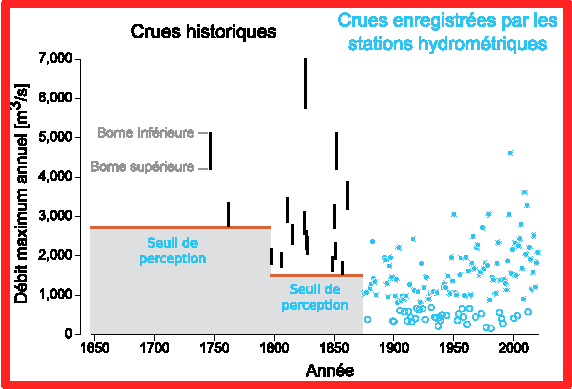
\includegraphics[width = .5\textwidth]{./Figures/HistoFloods1.pdf}
	\end{frame}	
	
 	\subsection{HISTRHÔNE (1300-2000)}
	%%%%%%%%% X %%%%%%%%%
	\begin{frame}%[c]
		\frametitle{Base de données HISTRHÔNE (1300-2000)}
		\centering
		Et avant les relevés systématiques ?\\
		\vfill
      	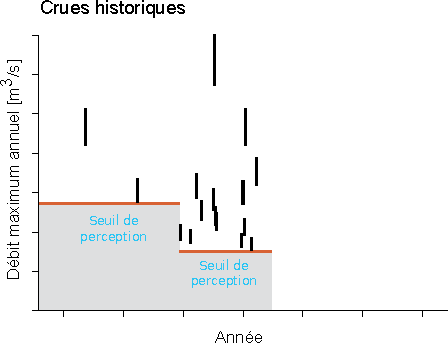
\includegraphics[width = .5\textwidth]{./Figures/HistoFloods2.pdf}
	\end{frame}	 	
 	
	%%%%%%%%% 23 %%%%%%%%%
	\begin{frame}%[c]
		\frametitle{Base de données HISTRHÔNE (1300-2000)}
\begin{minipage}{.45\textwidth}
			\begin{itemize}
				\item<1->[$\vartriangleright$] Base de données d'événements hydroclimatiques en basse vallée du Rhône \footfullcite{pichard_sept_2014}
				\vfill
				\item<2->[$\vartriangleright$] 1500 événements du XIII\textsuperscript{ème} siècle à 2000
				\vfill
				\item<3->[$\vartriangleright$] Classés par type et par gravité 
			\end{itemize}
		\end{minipage}
		\begin{minipage}{.54\textwidth}
			\begin{center}
	      		\includegraphics<1-2>[width = .65\textwidth]{./Figures/HistrhoneMap.jpg} 
	      		\includegraphics<3>[width = .62\columnwidth]{./Figures/CatHistrhone.png}\phantom{s}\\
				\vspace{1pt}				
				\tiny{Tiré de \url{histrhone.cerege.fr}} 
			\end{center}
		\end{minipage}
	\end{frame}

%%%%%%%%% X %%%%%%%%%
	\begin{frame}%[c]
		\frametitle{Base de données HISTRHÔNE (1300-2000)}
		\vfill		
		\centering
		Rhône gelé à Arles en 1929
		\vfill
		\includegraphics<1>[width = .8\textwidth]{./Figures/RhoneGele.jpg}
%      	\includegraphics<2>[width = .6\textwidth]{./Figures/HistoFloods2.pdf}
	\end{frame}	

\section{Incertitudes hydrométriques} 
	\subsection{Intro}
{
    \setbeamercolor{background canvas}{bg=myblue}
    \begin{frame}
        \begin{center}
        	\vfill
		 	\textcolor{white}{\large \textbf{1. Estimation des débits et incertitudes}}\\
		 	\vspace{0.5cm}
		 	\textcolor{white}{\large \textbf{Comment estimer et propager les différentes sources d'incertitude hydrométrique ?}}\\
			\vfill
			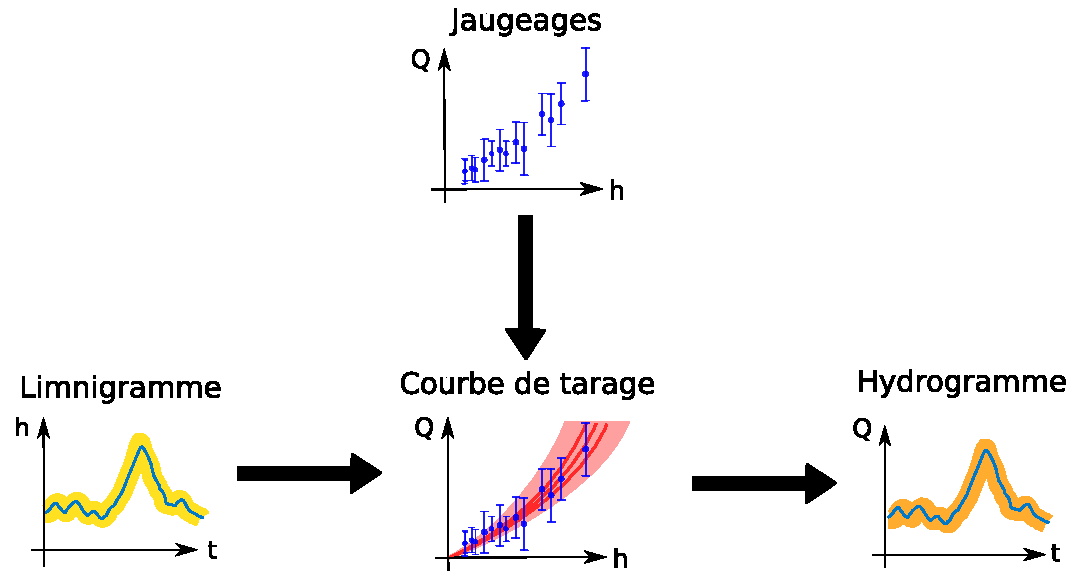
\includegraphics[width = .6\textwidth]{./Figures/Hydrom4.pdf}
        \end{center}
    \end{frame}
    }
    
  
    \subsection{Segm}
	%%%%%%%%% 12 %%%%%%%%%
	\begin{frame}%[c]
		\frametitle{Détarages}
		\centering
		Ruptures dans la relation hauteur/débit\\
		\vfill
		\begin{center}
			\includegraphics<1>[width = .45\textwidth]{./Figures/Detar1.pdf} 
			\includegraphics<2>[width = .45\textwidth]{./Figures/Detar2.pdf} 
		\end{center}
	\end{frame}
	
		\begin{frame}%[c]
		\frametitle{Détarages}
		Méthode itérative de détection des détarages \footfullcite{darienzo_detection_2021} \\
		\vspace{15pt}
		\begin{center}
			\includegraphics<1>[width = .9\textwidth]{./Figures/Segm1.pdf} 
			\includegraphics<2>[width = .9\textwidth]{./Figures/Segm2.pdf} 
			\includegraphics<3>[width = .9\textwidth]{./Figures/Segm3.pdf} 
			\includegraphics<4>[width = .9\textwidth]{./Figures/Segm4.pdf} 
			\includegraphics<5>[width = .9\textwidth]{./Figures/Segm5.pdf} 
		\end{center}
		\vfill
		\begin{itemize}
			\item<1->[$\vartriangleright$] Prise en compte de l'incertitude des résidus
			\vfill
			\item<2->[$\vartriangleright$] Itérations pour chacune des sous-périodes
		\end{itemize}
	\end{frame}
    
    
	\begin{frame}
		\frametitle{Segmentation des jaugeages}
		\vfill		
		\begin{minipage}{0.2\textwidth}
			\centering
			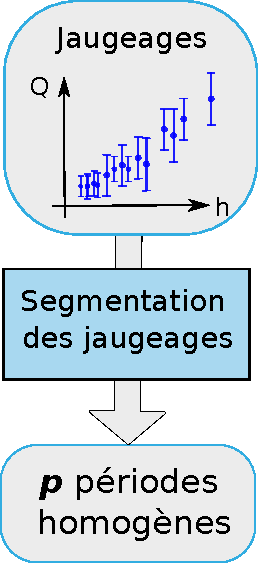
\includegraphics[width = .9\textwidth]{./Figures/SchemSegm.pdf} 
		\end{minipage}
		\hfill
		\begin{minipage}{0.78\textwidth}
			\centering
			Segmentation des jaugeages\footfullcite{darienzo_detection_2021} à Pont de Beaucaire
			\vfill
			\begin{center}
				\includegraphics<1>[width = .9\textwidth]{./Figures/Jaus.pdf} 
				\includegraphics<2>[width = .9\textwidth]{./Figures/SegmPt.pdf} 
			\end{center}
		\end{minipage}	
	\end{frame}
	
	\subsection{Courbes de tarage}
	%%%%%%%%% 12 %%%%%%%%%	
	\begin{frame}
    	\frametitle{Estimation des courbes de tarage}
		Estimation bayésienne des paramètres de la courbe de tarage : \textbf{BaRatin}\footfullcite{le_coz_combining_2014}\\
		\vfill
		\begin{center}
			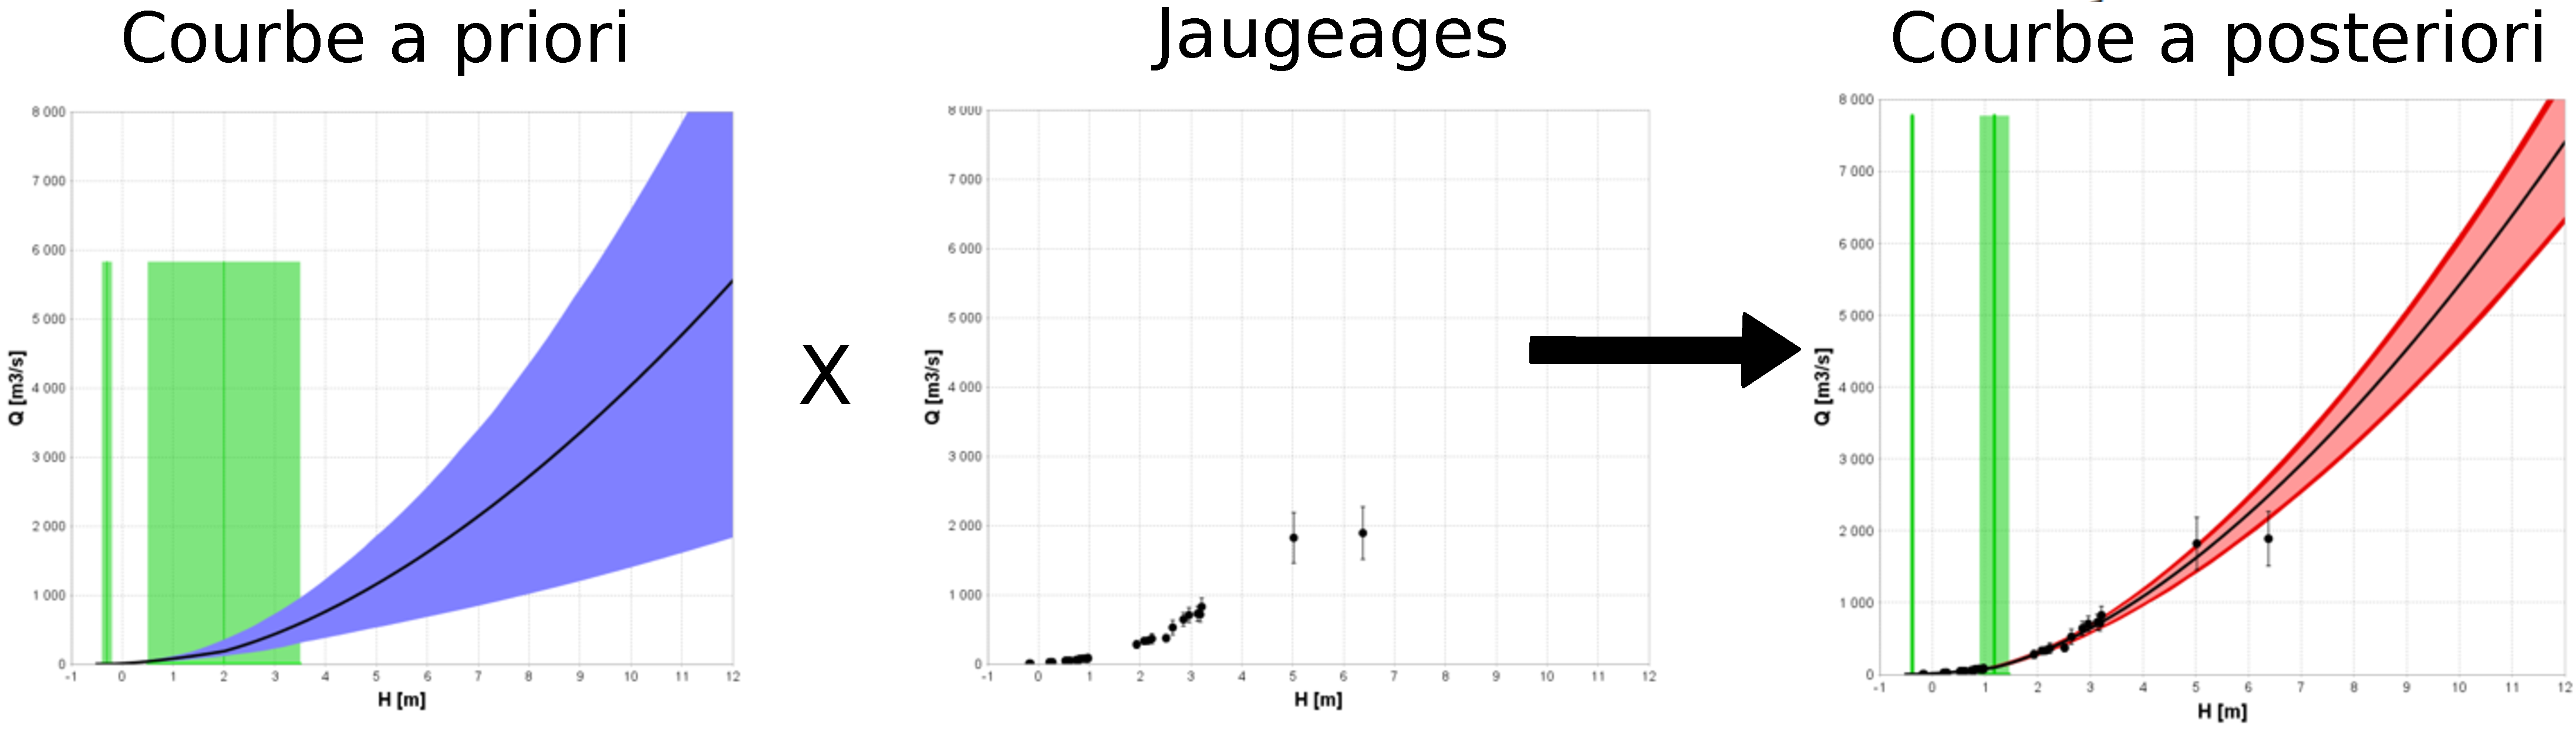
\includegraphics[width = .8\textwidth]{./Figures/Baratin.pdf} 
		\end{center}
		\begin{itemize}
			\item<1->[$\vartriangleright$] Courbe \textbf{\textit{a priori}} $\rightarrow$ connaissance hydraulique de la station : études de cartes/profils en travers\\		
			\vspace{5pt}
			\item<2->[$\vartriangleright$] Courbe \textbf{\textit{a posteriori}} $\rightarrow$ combinaison courbe \textbf{\textit{a priori}} et jaugeages \\		
		\end{itemize}		
	\end{frame}	
	
	\begin{frame}
		\frametitle{Estimation des courbes de tarage}
		\vfill		
		\begin{minipage}{0.2\textwidth}
			\centering
			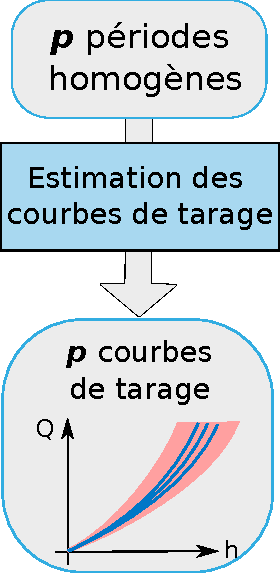
\includegraphics[width = .9\textwidth]{./Figures/SchemCT.pdf} 
		\end{minipage}
		\hfill
		\begin{minipage}{0.78\textwidth}
			\centering
			Estimation multipériode des courbes de tarage \footfullcite{mansanarez_shift_2019} :\\
			10 courbes de tarage à Pont de Beaucaire
			\begin{center}
				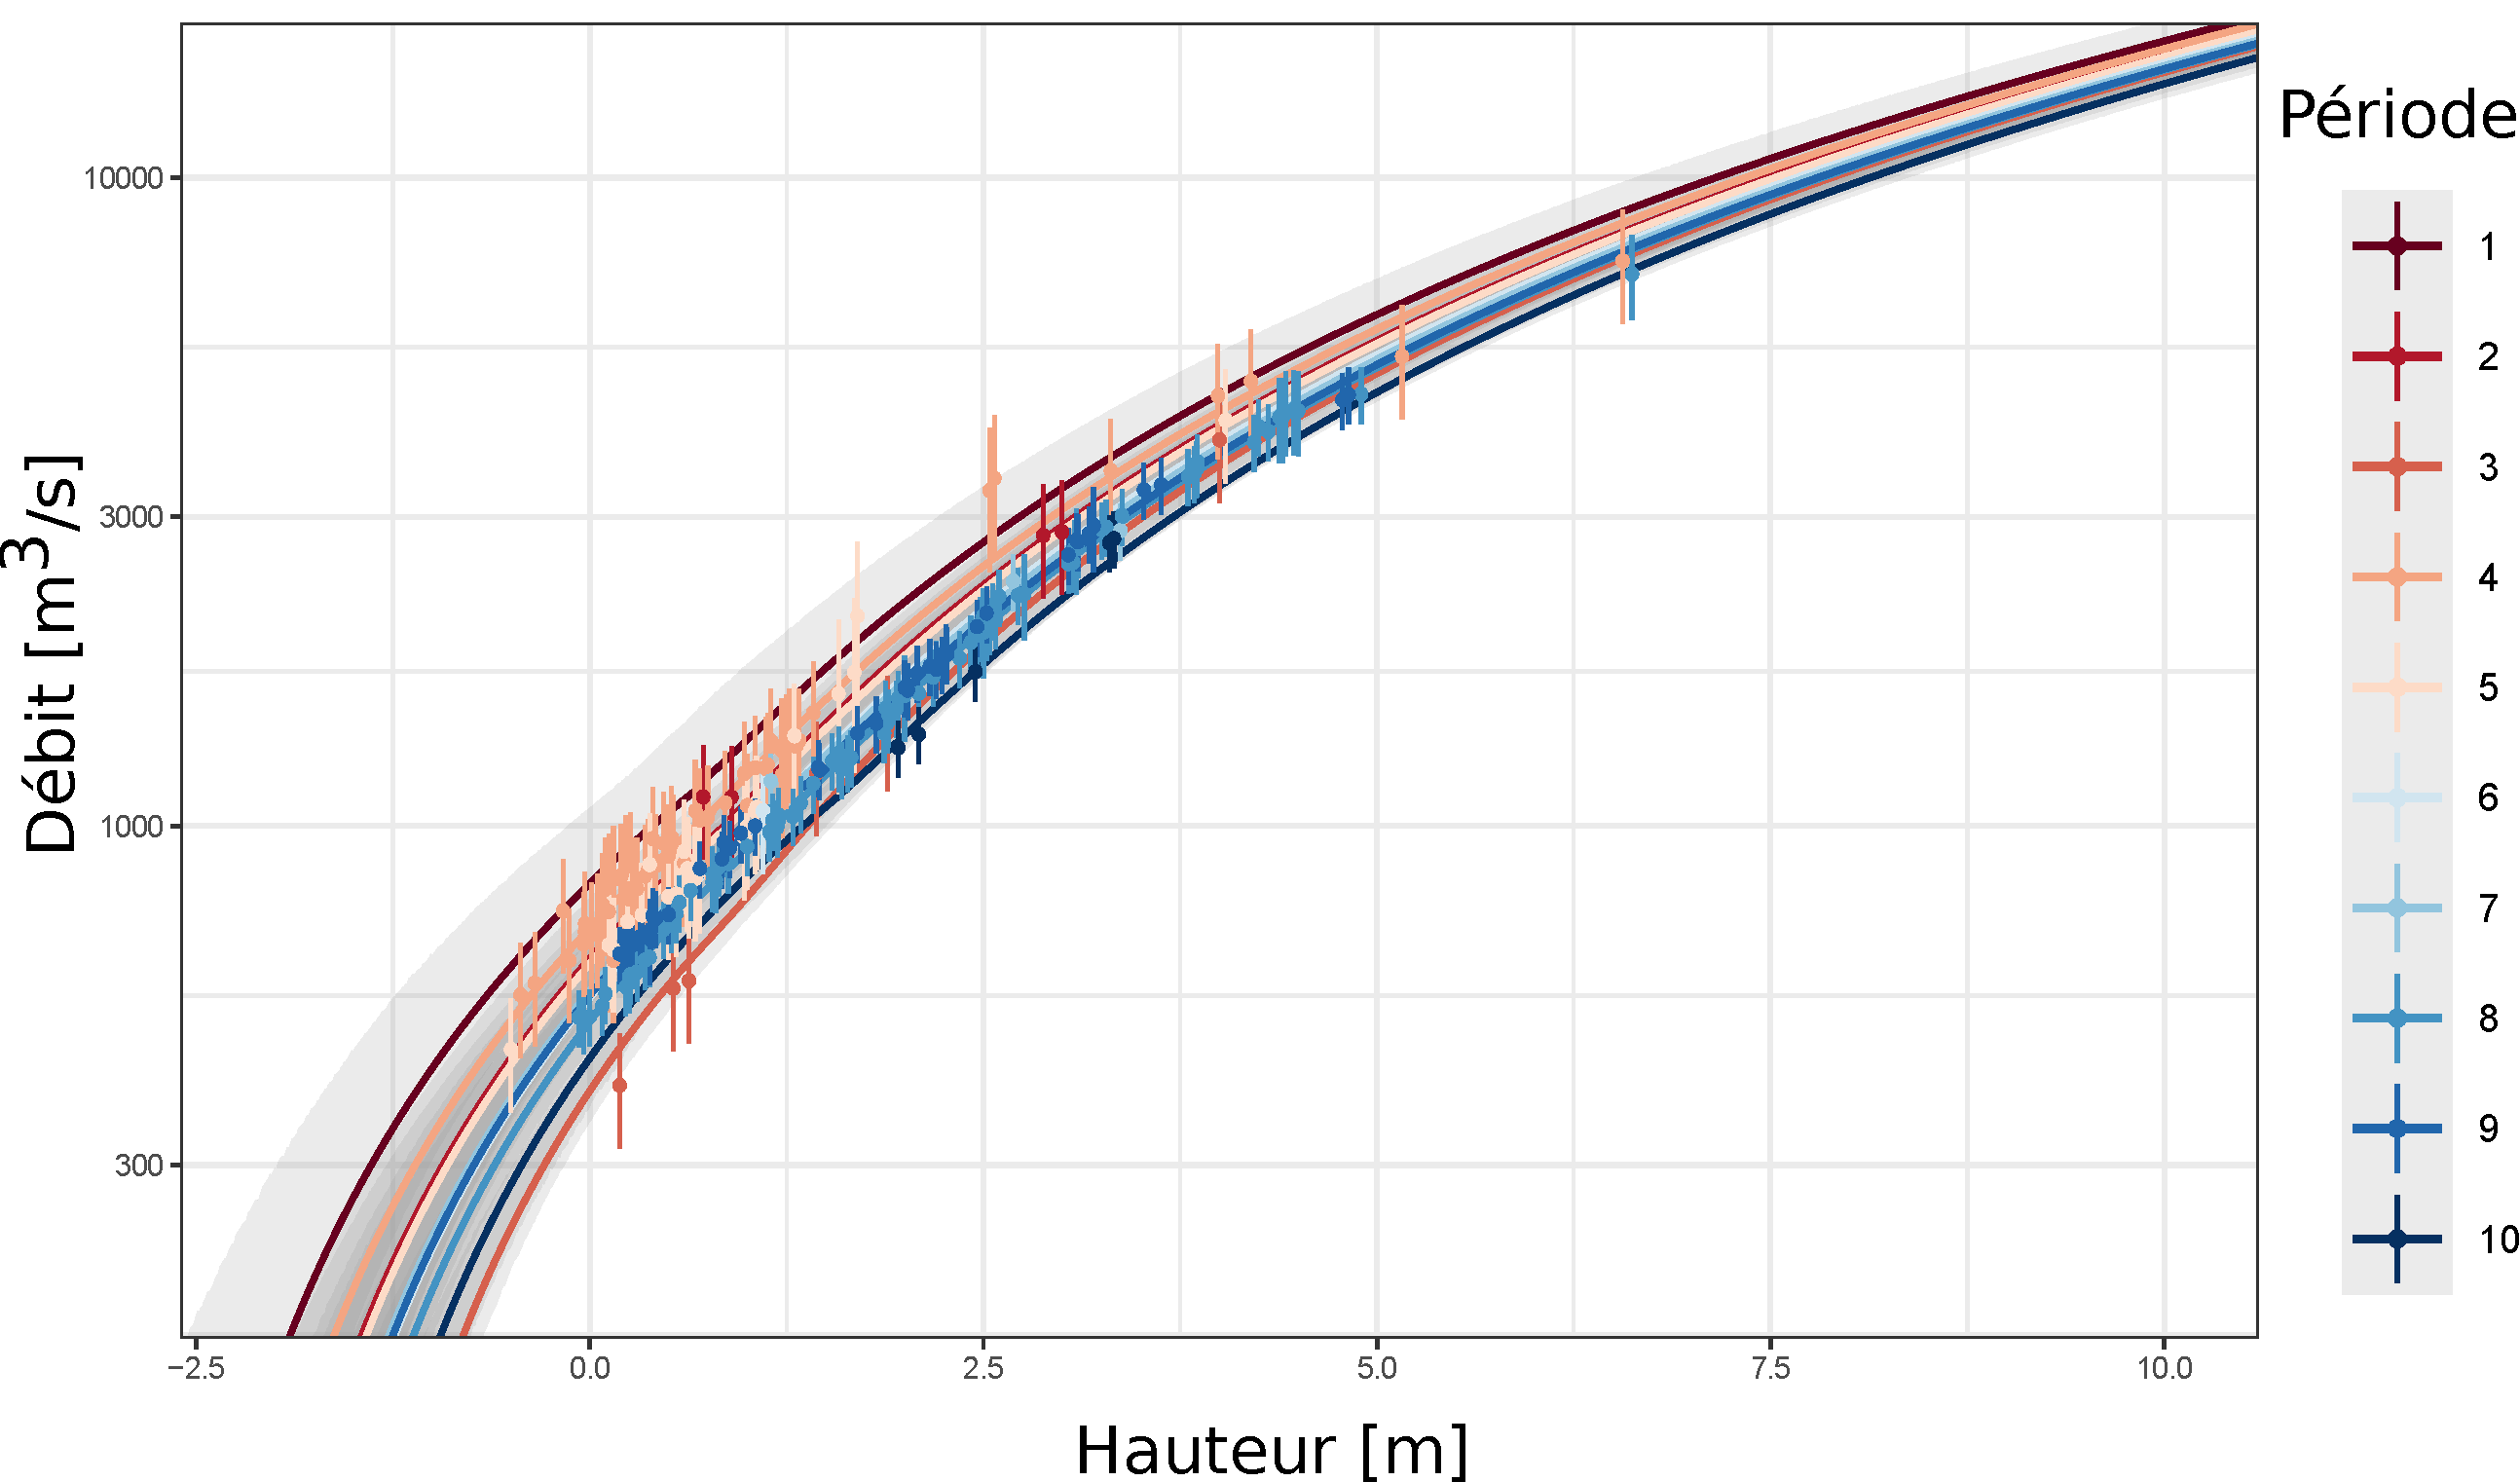
\includegraphics[width = .8\textwidth]{./Figures/RClogPt.pdf}  	
			\end{center}
%			\vfill
			\begin{itemize}
				\item<1->[$\vartriangleright$] Paramètres constants entre périodes $\Rightarrow$ expertise hydraulique
				\vfill
				\item<2->[$\vartriangleright$] Transfert d'informations entre périodes $\Rightarrow$ expression d'une vraisemblance commune aux $p$ périodes
				\vfill
			\end{itemize}
		\end{minipage}
	\end{frame}
	
%	\begin{frame}
%		\frametitle{Estimation des courbes de tarage}
%		\vfill		
%		\begin{minipage}{0.2\textwidth}
%			\centering
%			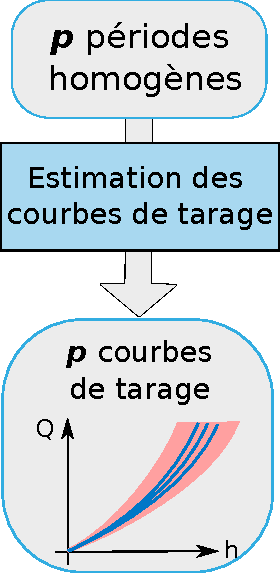
\includegraphics[width = .9\textwidth]{./Figures/SchemCT.pdf} 
%		\end{minipage}
%		\hfill
%		\begin{minipage}{0.78\textwidth}
%			\centering
%			Courbes de tarage à Pont de Beaucaire
%			\vfill
%			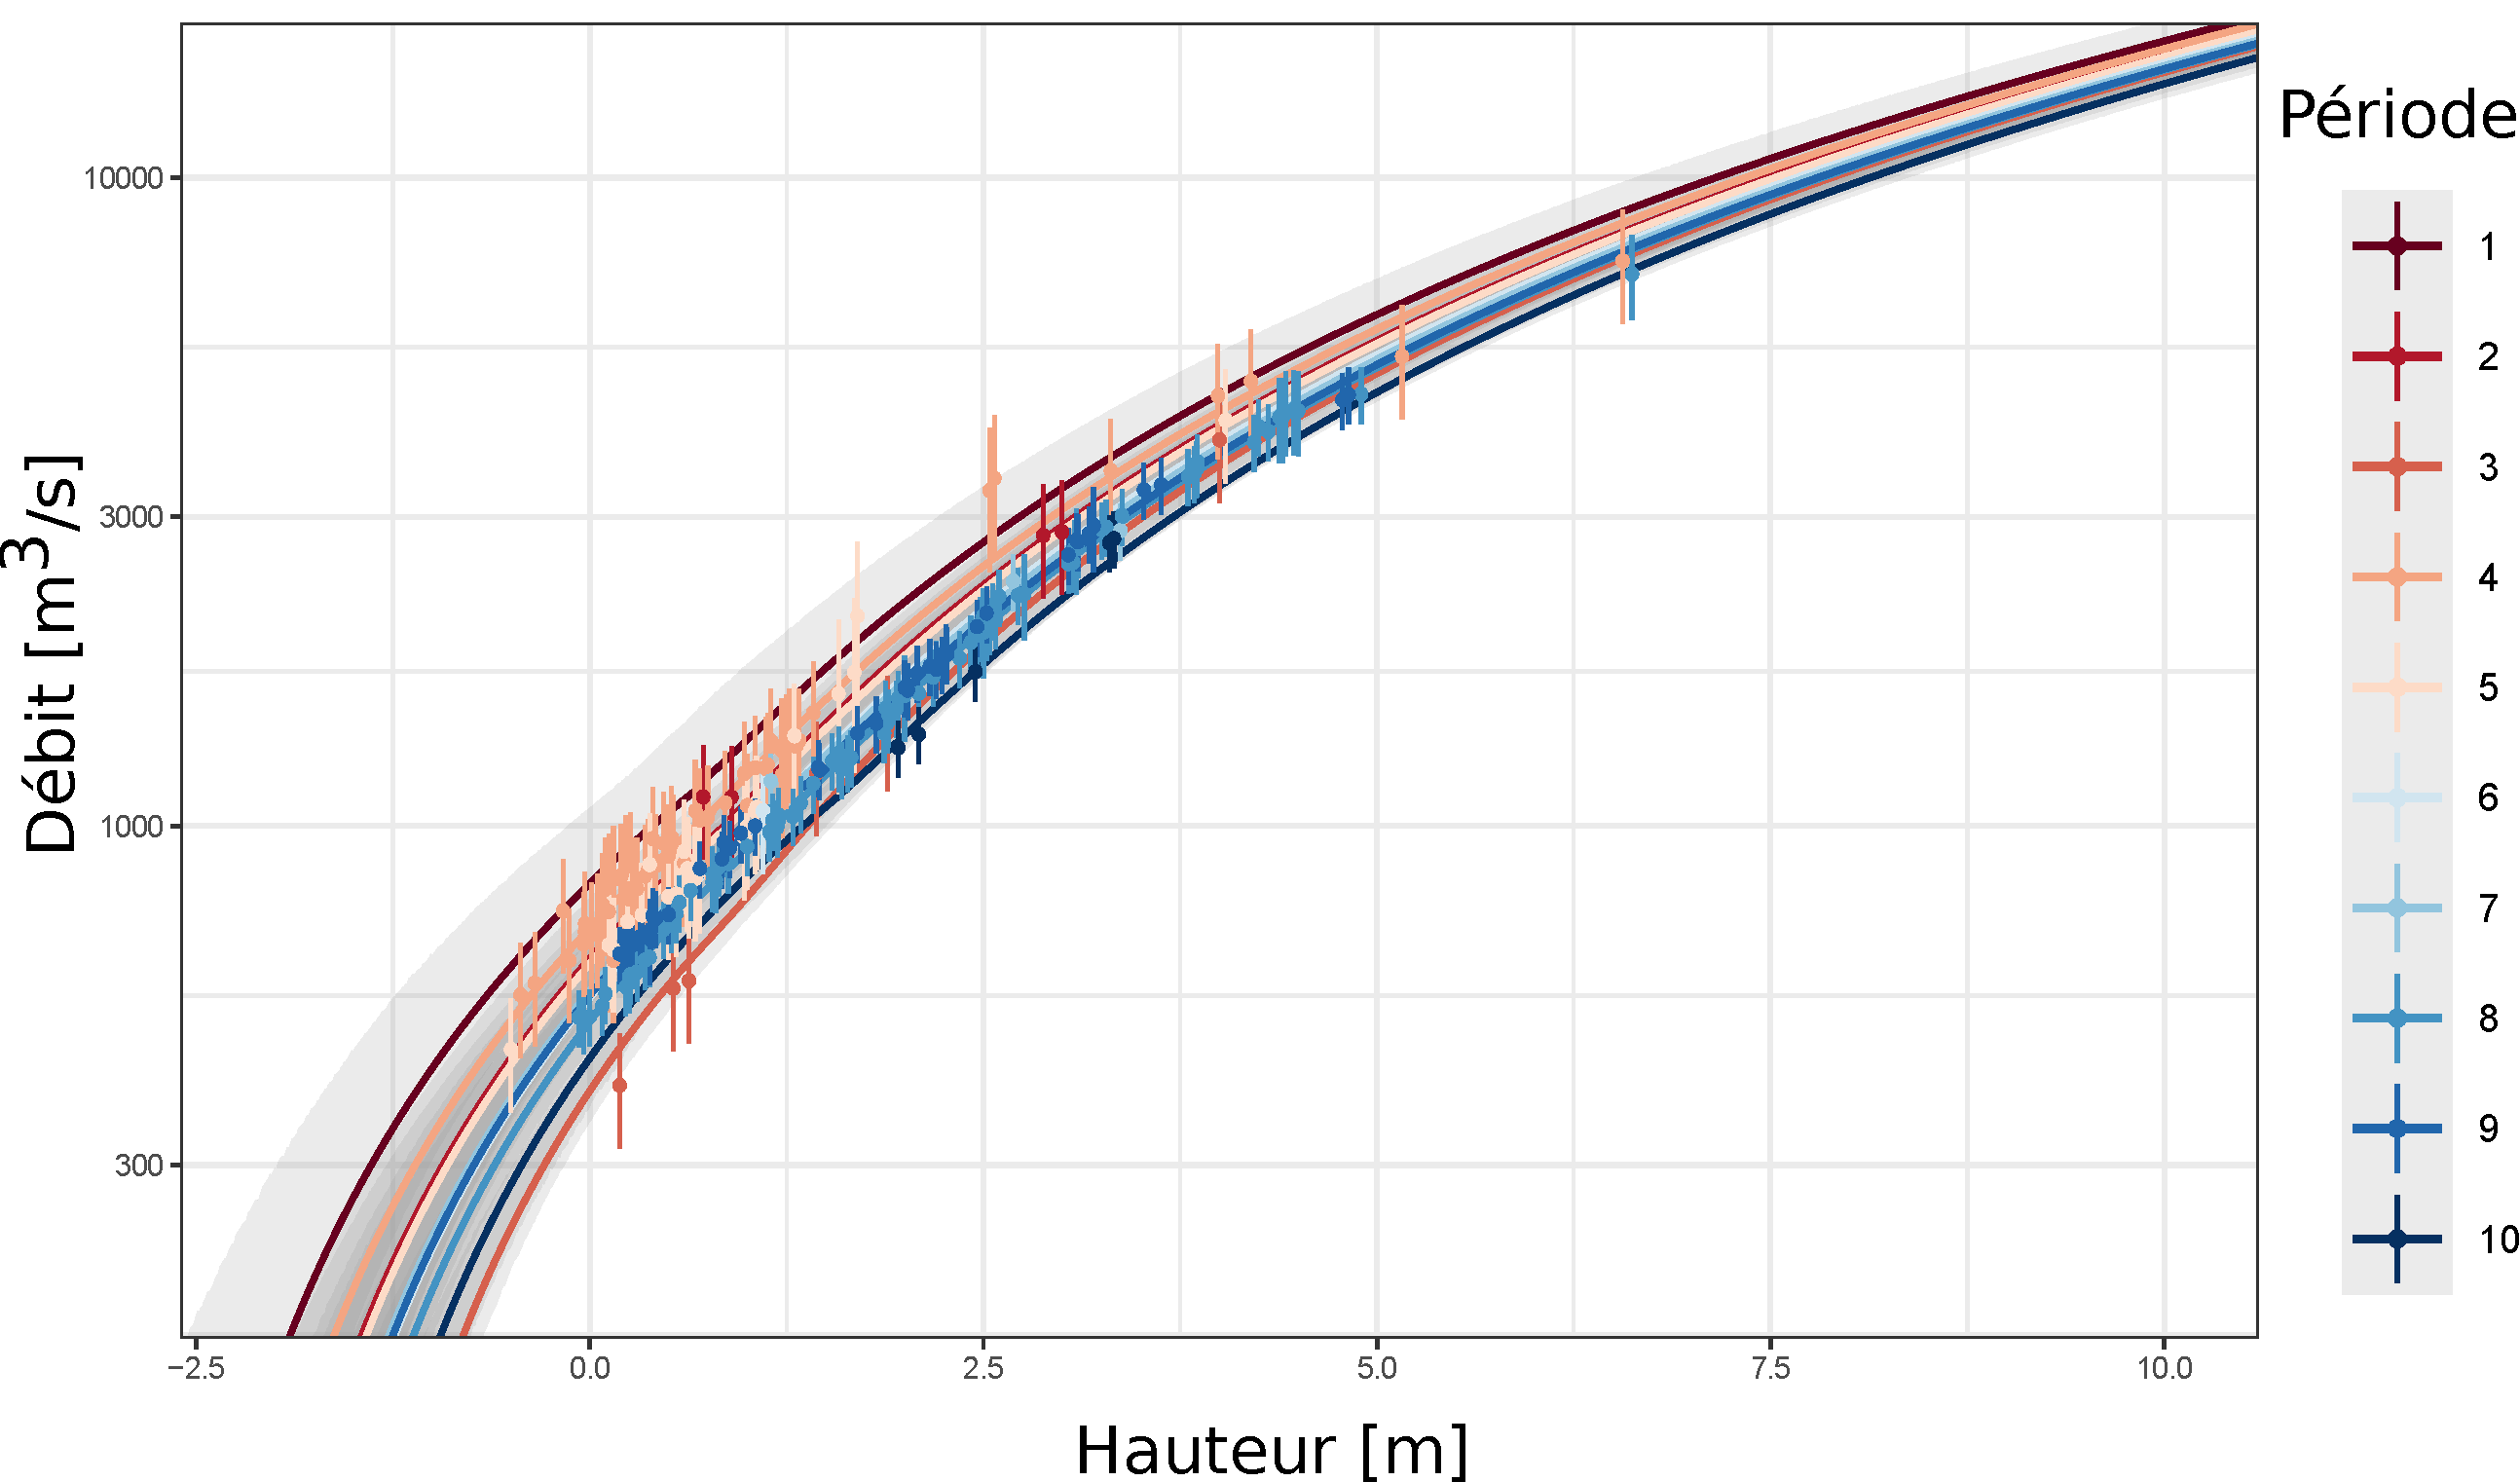
\includegraphics[width = \textwidth]{./Figures/RClogPt.pdf}  	
%		\end{minipage}
%	\end{frame}}
	
	\subsection{Limnigrammes incertains}
	
%	\begin{frame}
%		\frametitle{Incertitude limnimétrique}
%		\begin{minipage}{0.2\textwidth}
%			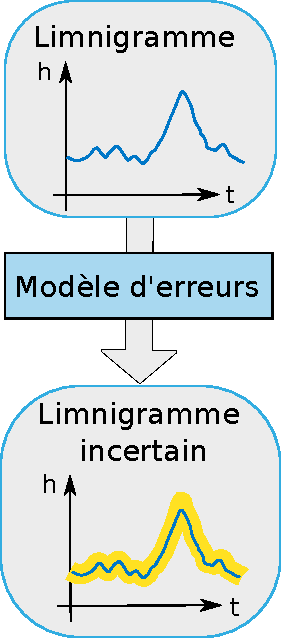
\includegraphics[width = .9\textwidth]{./Figures/SchemLimni.pdf} 
%		\end{minipage}
%		\hfill
%		\begin{minipage}{0.78\textwidth}
%			Incertitude résultant de 5 erreurs additives : 
%			\vfill		
%			\begin{equation}
%				\hbar(t) = h(t) + \delta_1(t) +\delta_2(t)+\delta_3(t)+\delta_4(t)+\delta_5(t)
%			\end{equation}
%			\vfill
%			Où $\hbar$ est la vraie hauteur inconnue et $h$ la hauteur mesurée\\
%			\vfill
%			\begin{itemize}
%				\item<2->[$\vartriangleright$] Lecture visuelle de l'échelle : $\delta_1 \sim \mathcal{N}(0,0.5)$
%				\item<3->[$\vartriangleright$] Incertitude du capteur : $\delta_2 \sim\mathcal{N}(0,0.01/\sqrt{3})$
%				\item<4->[$\vartriangleright$] Recalage capteur : $\delta_3 \sim \mathcal{N}(0,0.06)$
%				\item<5->[$\vartriangleright$] Mesure du zéro de l'échelle : $\delta_4 \sim \mathcal{N}(0,0.06)$\\
%				\item<6-> [$\vartriangleright$] \textbf{Fréquence des relevés} :\\ 
%				\onslide<7-> Relevés automatiques infra-horaires (1970-2020) : $\delta_5 = 0$\\
%				Relevés visuels 3 fois/jour (1840-1967) : $\delta_5 = 0$ si $h>5$m, \\
%				$\>$ $\>$ $\>$ $\>$ $\>$ $\>$ $\>$ $\>$ sinon $\delta_5 \sim \mathrm{Exp}(8.86)$\\
%				Relevé visuel 1 fois/jour (1816-1839) : $\delta_5 \sim \mathrm{Exp}(2.18)$\\
%			\end{itemize}
%			\vfill
%		\end{minipage}
%	\end{frame}	
	
	
	\begin{frame}
		\frametitle{Incertitude limnimétrique}
		\begin{minipage}{0.2\textwidth}
			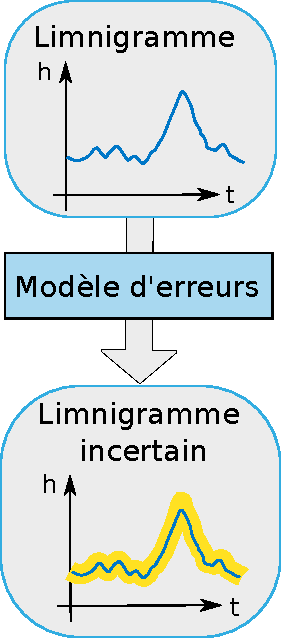
\includegraphics[width = .9\textwidth]{./Figures/SchemLimni.pdf} 
		\end{minipage}
		\hfill
		\begin{minipage}{0.78\textwidth}
			Modèle d'erreurs limnimétriques \footfullcite{horner_impact_2018}
			
			\begin{itemize}
				\item<2->[$\vartriangleright$] 4 termes d'erreur additifs : lecture de l'échelle, recalage du capteur...
				\item<3-> [$\vartriangleright$] Ajout d'un 5\textsuperscript{ème} terme : erreur due à la fréquence des relevés\\
				\vfill
				\begin{center}
					\includegraphics<4>[width =  .9\textwidth]{./Figures/uLimni1.pdf} 
					\includegraphics<5>[width = .9\textwidth]{./Figures/uLimni2.pdf} 			
				\end{center}
				\vfill
				\item<6->[$\vartriangleright$] \textbf{1816-1840} : 1 relevé/jour à 12h $\rightarrow$ $\delta_5 \sim \mathrm{Exp}(2.18)$\\
				\item<7->[$\vartriangleright$] \textbf{1841-1967} : 
				\begin{itemize}
						\item<7->[$\vartriangleright$] Si h > 5 m : relevés horaires $\rightarrow$ $\delta_5 = 0$
						\item<7->[$\vartriangleright$] Si h < 5 m : 3 relevés/jour $\rightarrow$ $\delta_5 \sim \mathrm{Exp}(8.86)$
				\end{itemize}								
				\item<8->[$\vartriangleright$] \textbf{après 1970} : relevés automatiques infra-horaires $\rightarrow$ $\delta_5 = 0$
			\end{itemize}
			\vfill
		\end{minipage}
	\end{frame}	
	
	\begin{frame}
		\frametitle{Incertitude limnimétrique}
		\begin{minipage}{0.2\textwidth}
			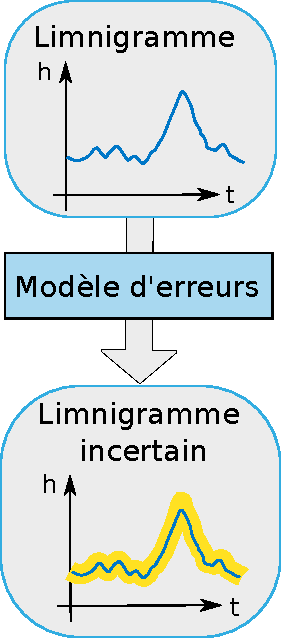
\includegraphics[width = .9\textwidth]{./Figures/SchemLimni.pdf} 
		\end{minipage}
		\hfill
		\begin{minipage}{0.78\textwidth}
			\centering
			Hauteurs maximum annuelles à Beaucaire (1816-2020)
			\vfill
			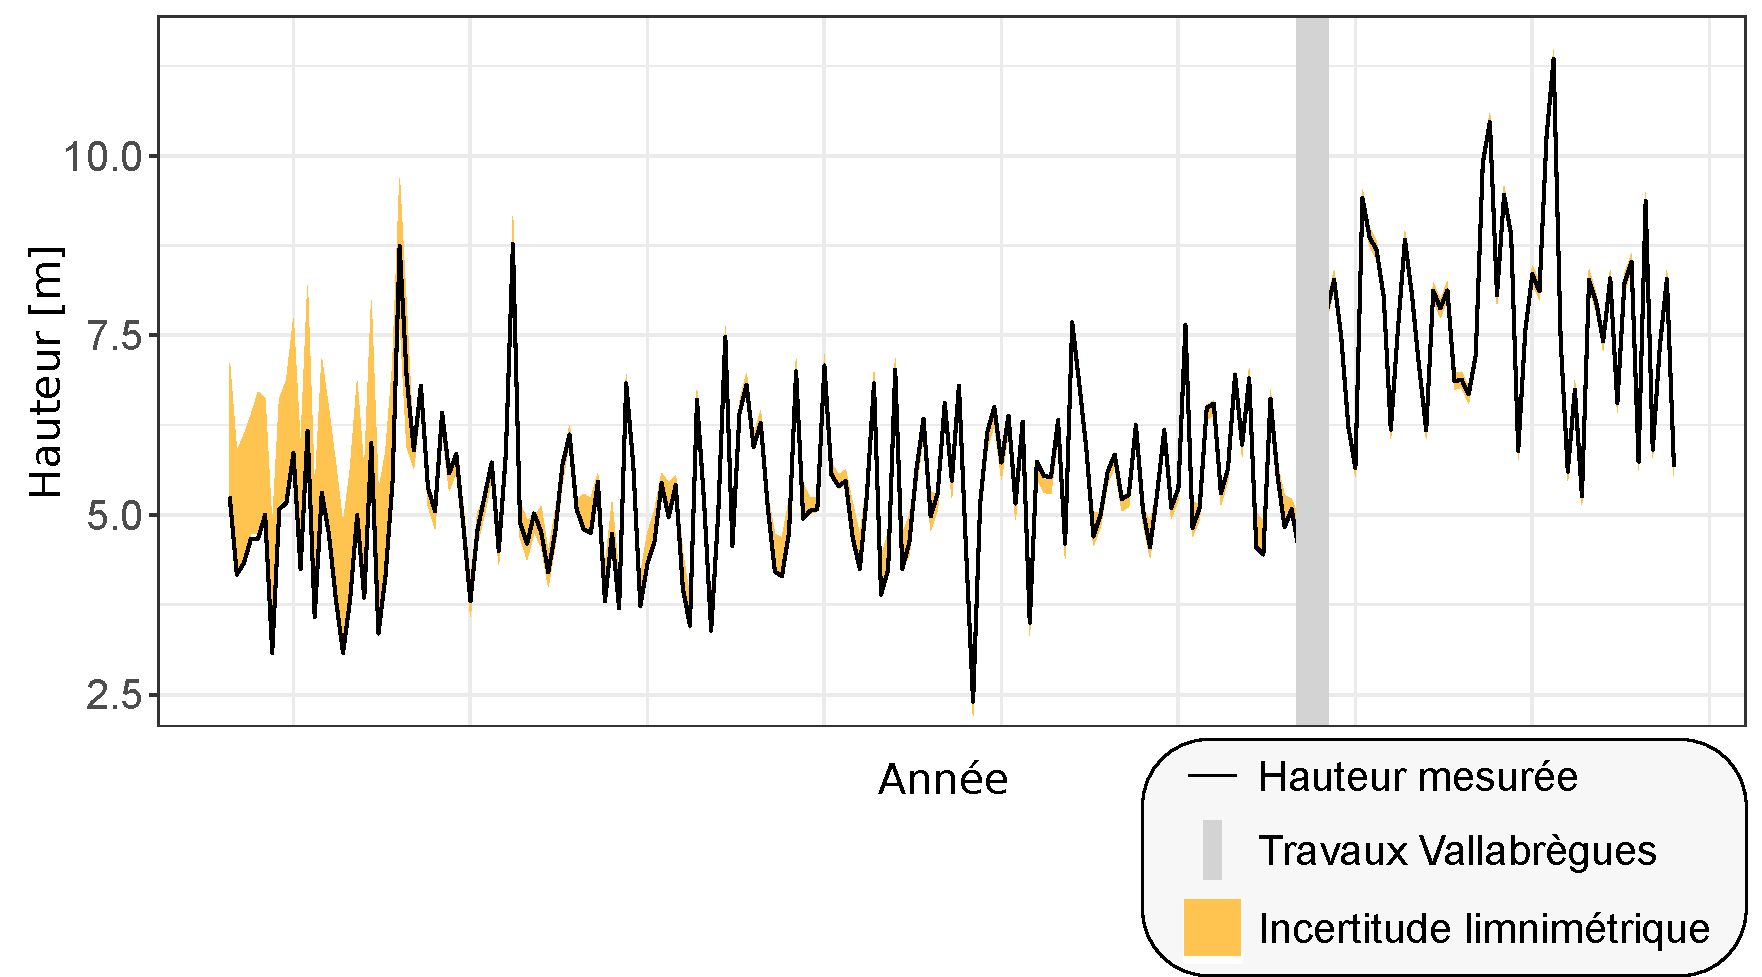
\includegraphics[width = \textwidth]{./Figures/Stage.pdf} 
		\end{minipage}
	\end{frame}	
	
	\begin{frame}
		\frametitle{Propagation des incertitudes}
		\begin{minipage}{0.2\textwidth}
			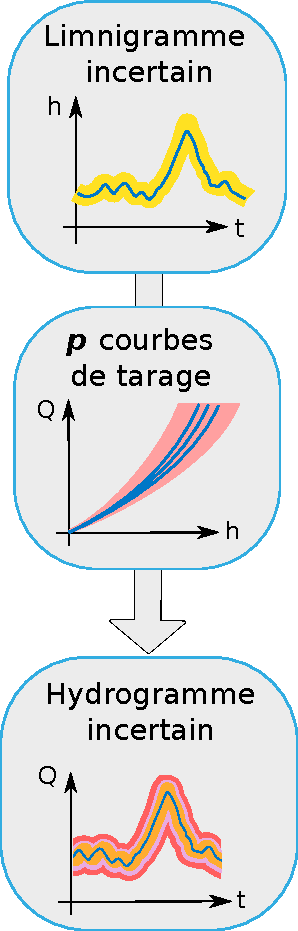
\includegraphics[width = .9\textwidth]{./Figures/SchemaHydrog.pdf} 
		\end{minipage}
		\hfill
		\begin{minipage}{0.78\textwidth}
			\centering
			Propagation successive des diverses sources d'incertitude\\
			\vspace{10pt}
			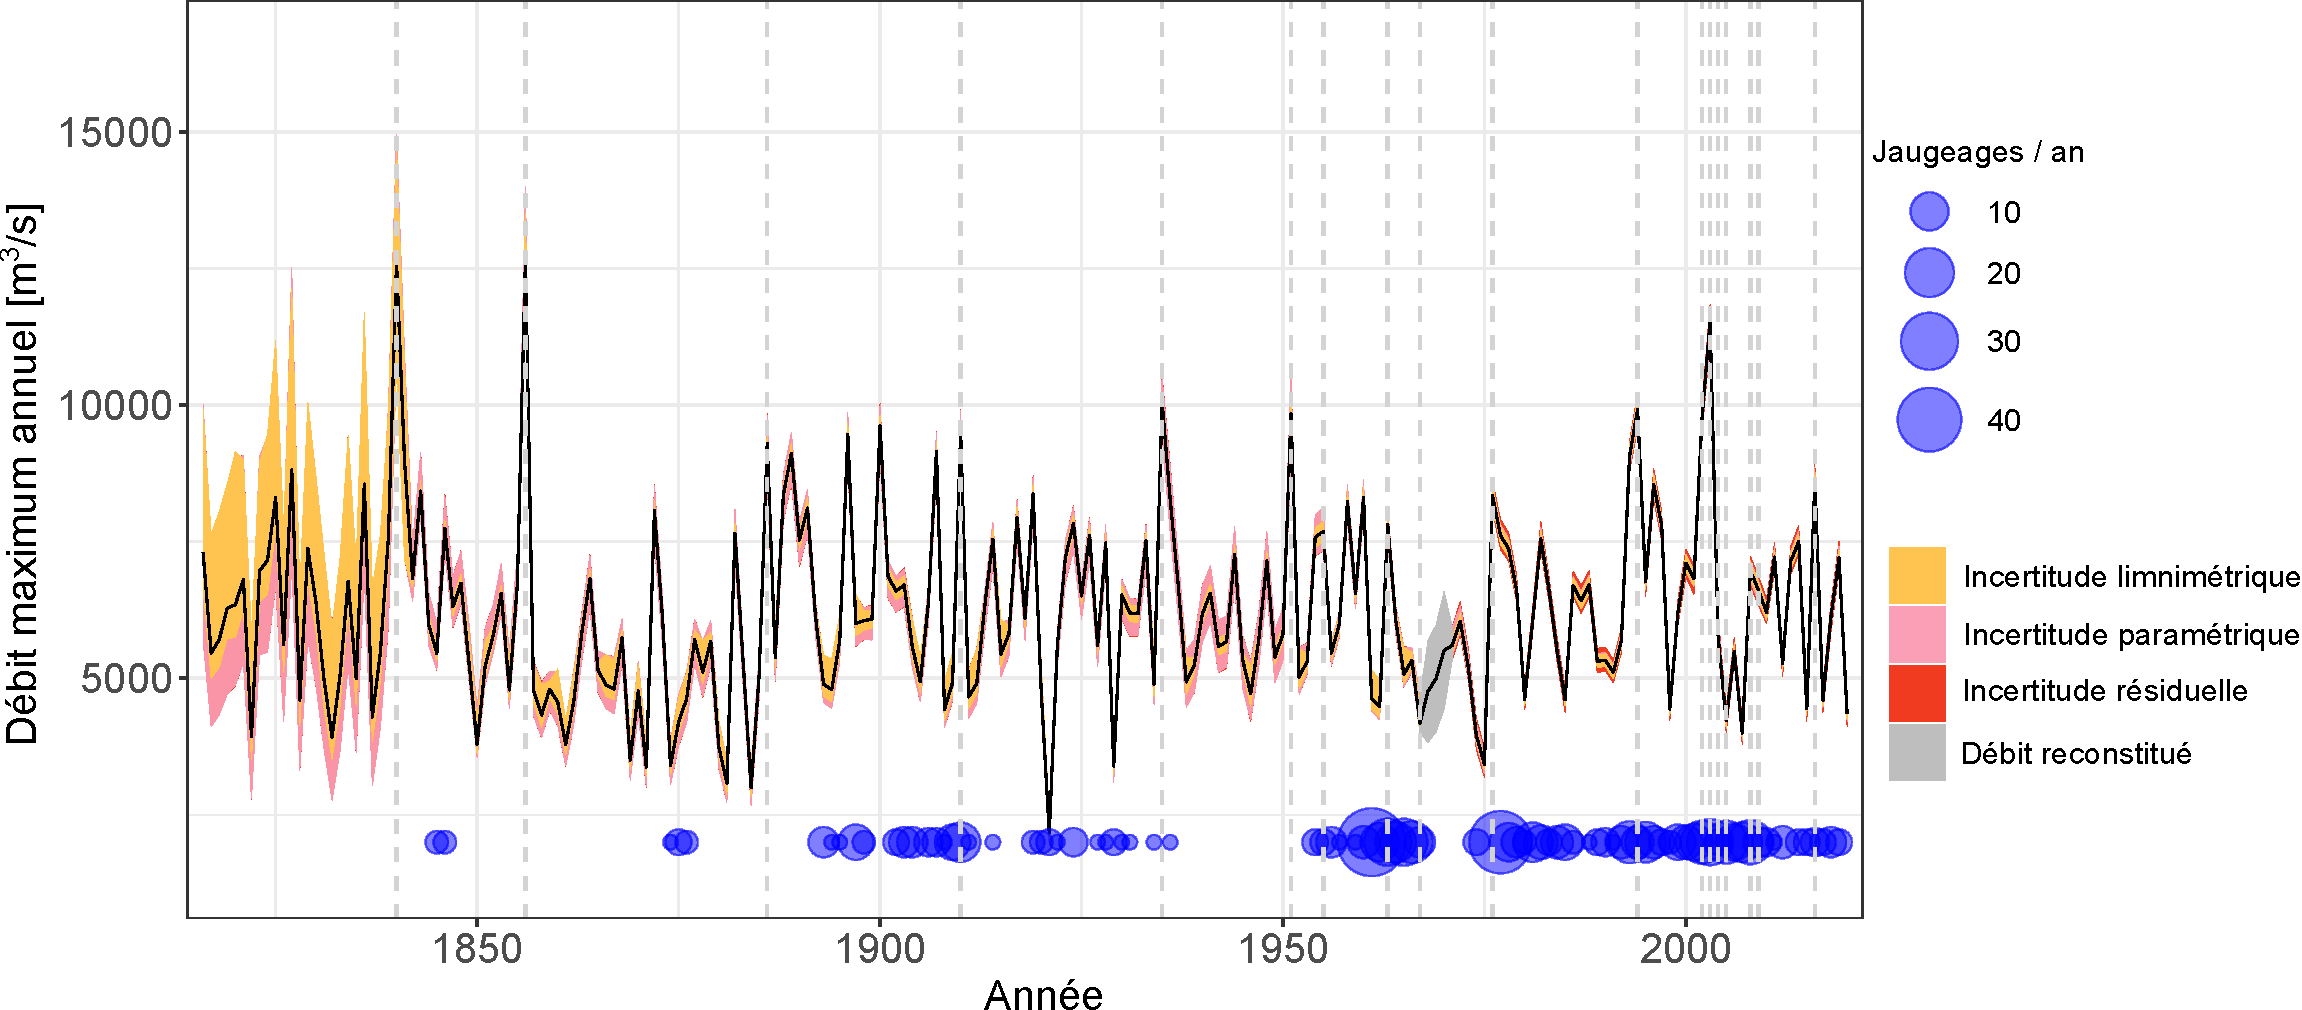
\includegraphics[width = \textwidth]{./Figures/uQ.pdf} 
			\centering
			\vspace{10pt}
			De $\pm$ 30\% à $\pm$ 5\% d'incertitude selon les périodes
		\end{minipage}
	\end{frame}	
		
	\subsection{Témoignages de crues (1500-2000)}
	\begin{frame}
		\frametitle{Témoignages de crues}
		\centering
		\includegraphics<1>[width = .6\textwidth]{./Figures/HistoFloods2.pdf} 		
	\end{frame}		
	
	\begin{frame}[t]
		\frametitle{Témoignages de crues (1500-2000)}
		\vfill
		\textbf{Catégorie C4, crue et inondation
extrêmes} $\Rightarrow$ \og \textit{Inondation extraordinaire avec dégâts exceptionnels (pertes humaines et animales, intérieurs des villes inondés [...]}\fg{}  
	\vfill
		\begin{itemize}
			\item<2->[$\vartriangleright$] Ordre de grandeur ? \citet{pichard_hydro-climatology_2017} $\Rightarrow$ 9000 $m^3/s$ 
			\item<3->[$\vartriangleright$] Modélisation hydraulique ? $\Rightarrow$ Calcul incertitudes ? Bathymétrie ancienne ?
			\item<4->[$\vartriangleright$] Croisement données HISTRHÔNE \textbf{(1500-2000)} et série de débits  \textbf{(1816-2020)}
		\end{itemize}
		\vfill
		\centering
		\includegraphics<5>[width = .75\textwidth]{./Figures/C4_SystematicPeriod-FR.pdf} 	
	\end{frame}		
		
	\subsection{Conclusion estimation débits}
	\begin{frame}[t]
		\frametitle{Conclusion}
		\vfill
		\centering
		\large{\textbf{Q.1 - Comment estimer et propager les différentes sources d'incertitude
hydrométrique ?}}
		\vfill
		\normalsize
		\begin{itemize}
			\item<1->[$\vartriangleright$] Création d'une chaine de propagation des incertitudes hydrométriques
			\vspace{10pt}
			\item<2->[$\vartriangleright$] Estimation des débits maximum annuels incertains $\rightarrow$ 1816 - 2020
			\vspace{10pt}
			\item<3->[$\vartriangleright$] Incertitude totale de $\pm$ 30\% à $\pm$ 5\% 
			\vspace{10pt}
			\item<4->[$\vartriangleright$] Collecte de témoignages de crues historiques catégorie C4 $\rightarrow$ 1500 - 1816
			\vspace{10pt}
			\item<5->[$\vartriangleright$] Première estimation de l'ordre de grandeur du débit relatif au seuil de perception des crues C4
		\end{itemize}
	\end{frame}
	
	\begin{frame}
		\frametitle{Conclusion}
		\vfill
		\centering
		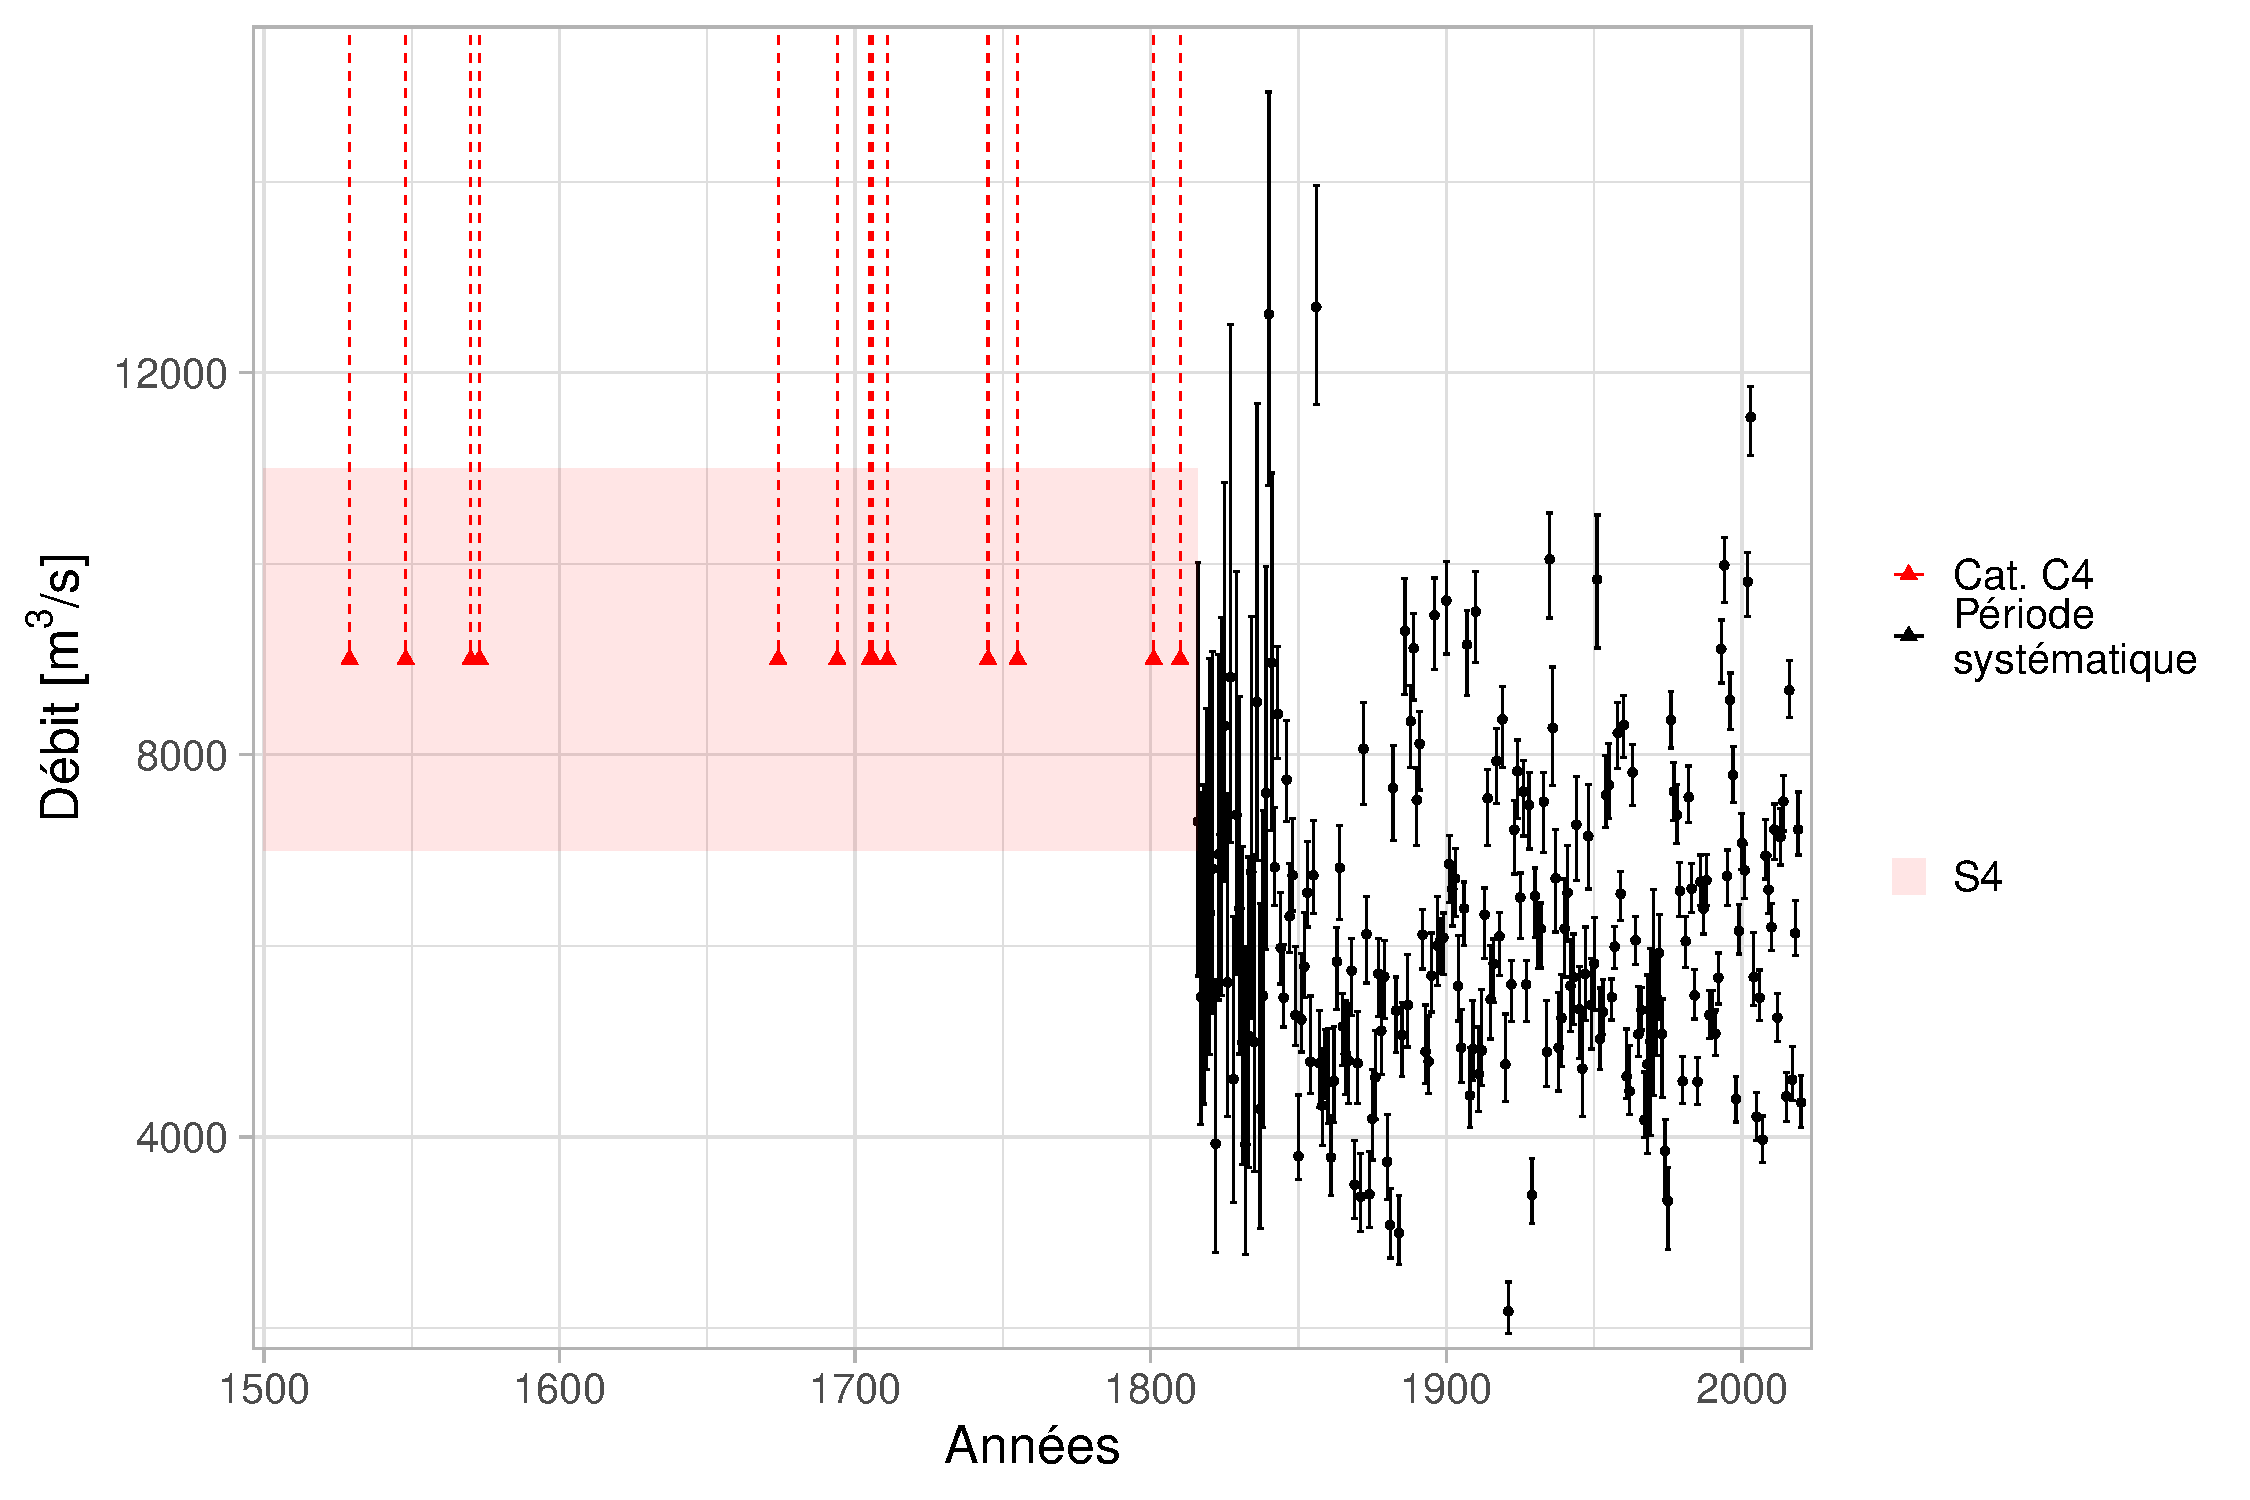
\includegraphics[width = .9\textwidth]{./Figures/EchMixteC4Bcr.pdf} 
	\end{frame}

\section{Hydrométrique vs Échantillonnage}
	\subsection{Intro}
	{
    \setbeamercolor{background canvas}{bg=myblue}
    \begin{frame}
        \begin{center}
        	\vfill
        	\textcolor{white}{\Large \textbf{Incertitude hydrométrique vs. incertitude d'échantillonnage}}\\
		\vfill
		\textcolor{white}{\large \textbf{Comment estimer la part respective de l'incertitude hydrométrique et de l'incertitude d'échantillonnage dans l'incertitude totale des quantiles ?\\
		\vspace{0.5cm}
		Jusqu'à quelle limite l'utilisation de limnigrammes anciens permet de réduire l'incertitude des quantiles de crue ?
		}}
		\vfill
	 	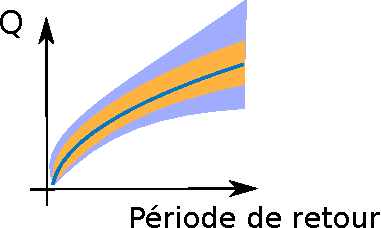
\includegraphics[width = .3\textwidth]{./Figures/Qpart.pdf} 
        \end{center}
    \end{frame}
    }

	\subsection{Période systématique (1816-2020)}
	\begin{frame}
		\frametitle{Analyse fréquentielle 1816-2020}
		\centering
		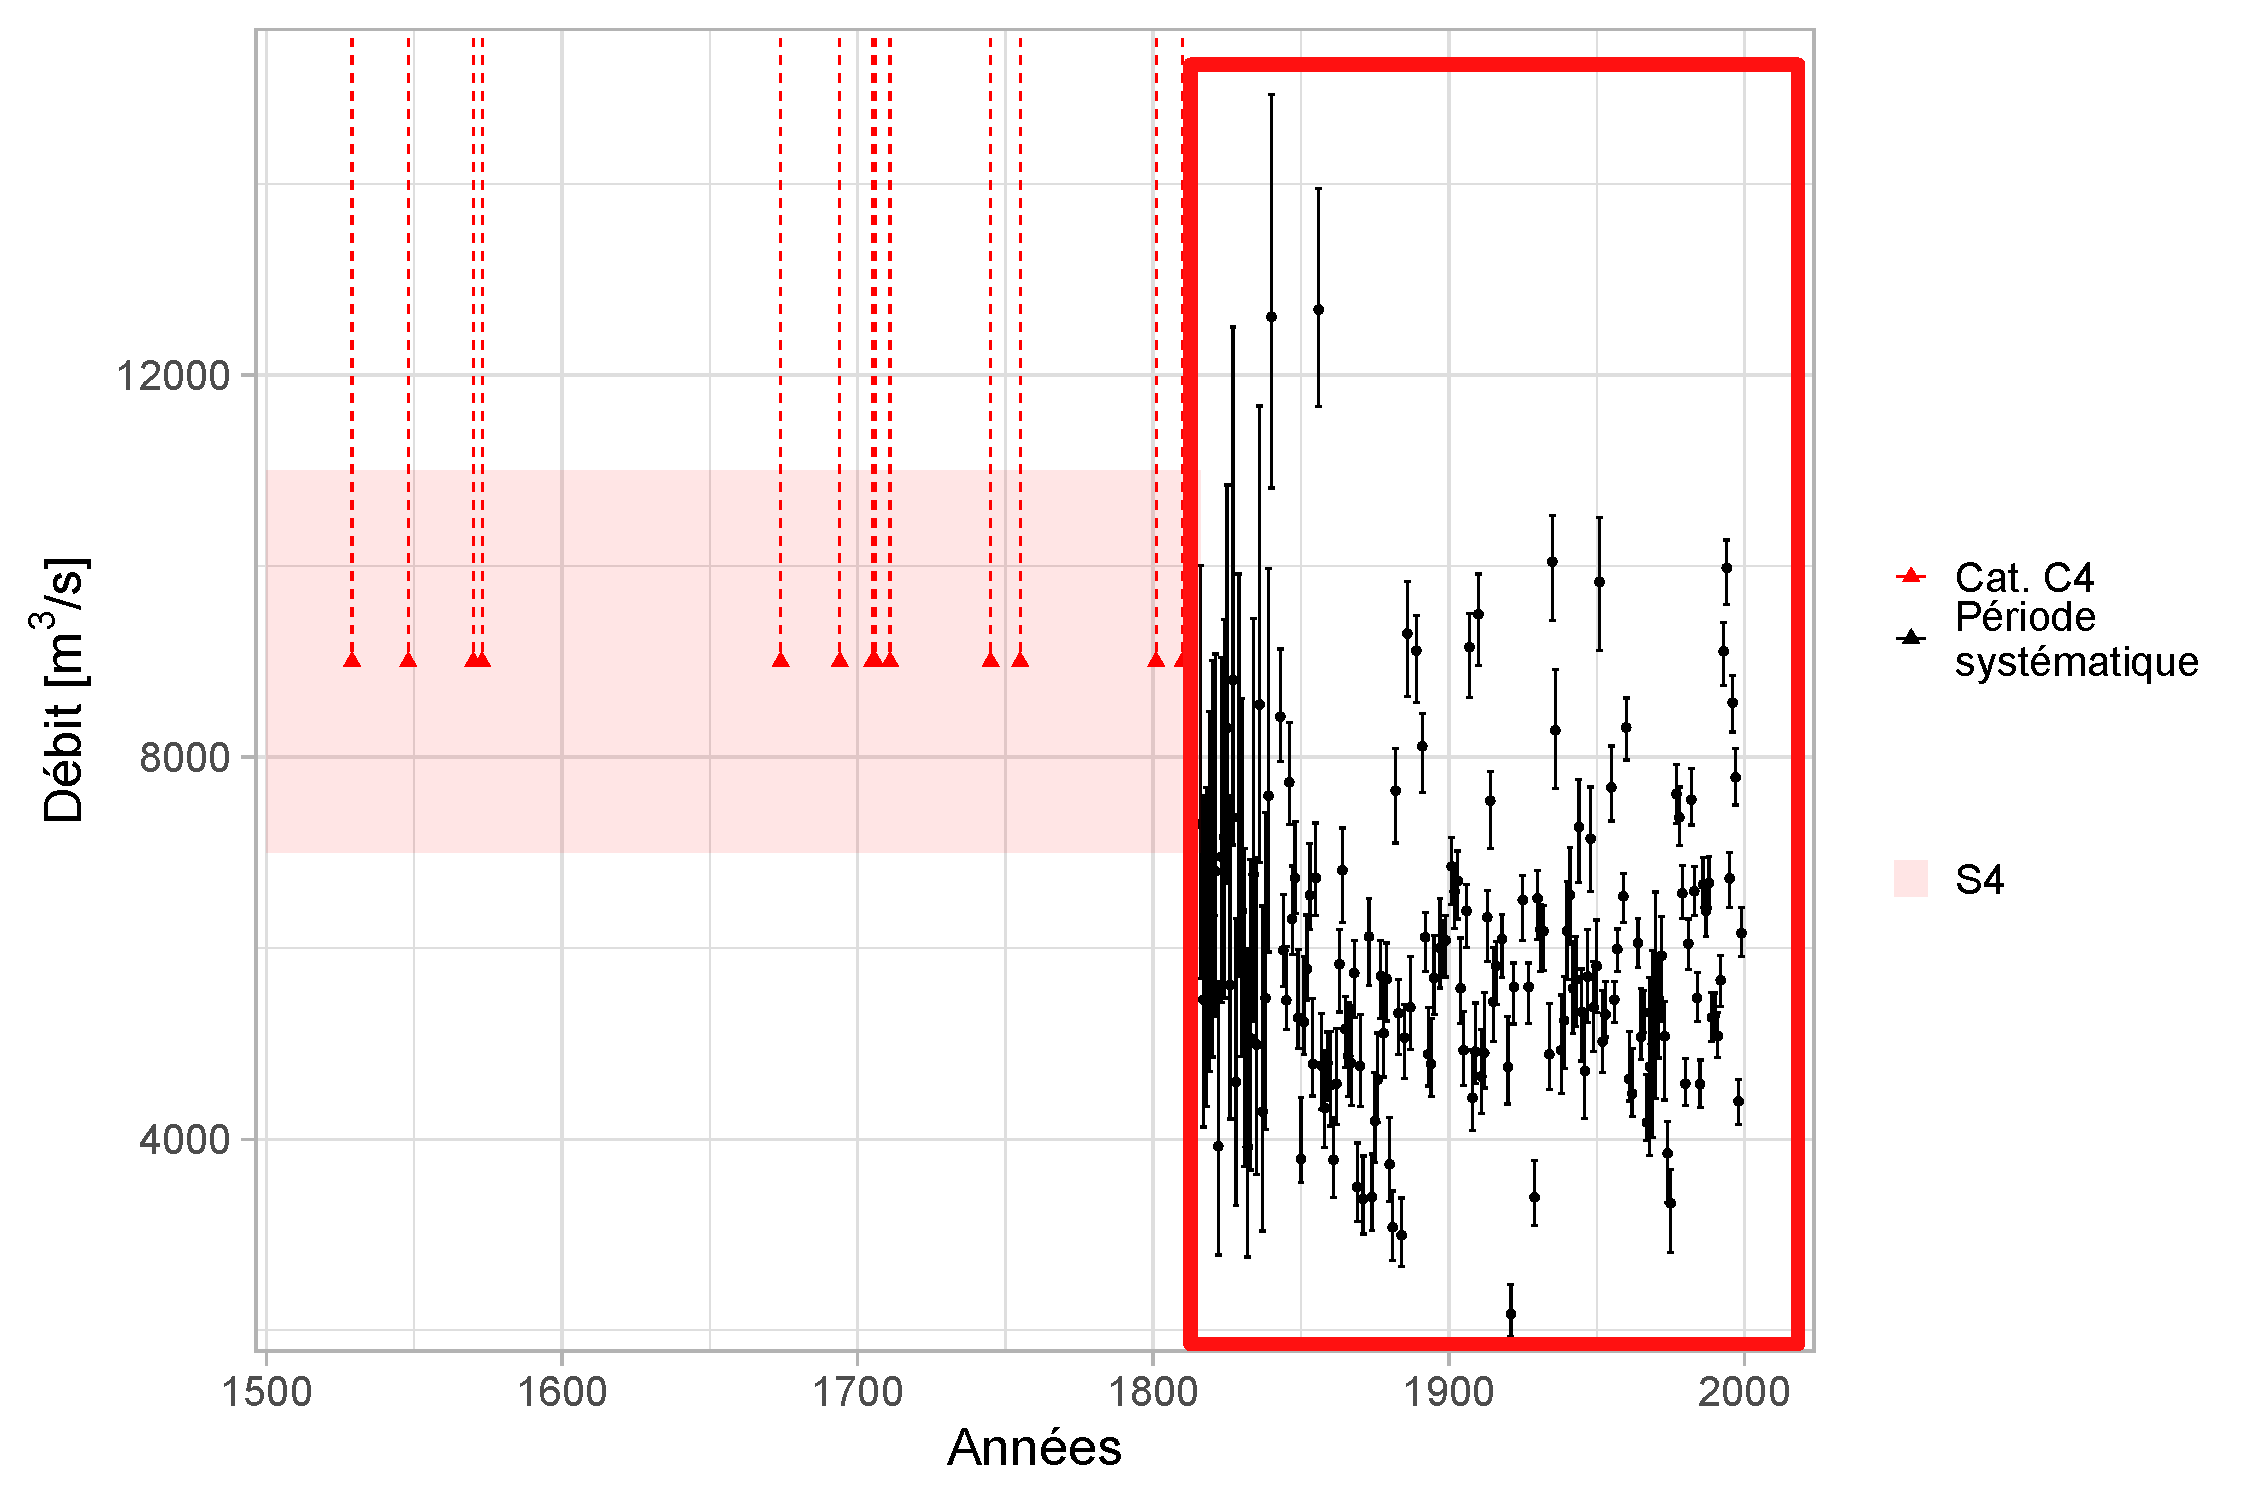
\includegraphics[width = .9\textwidth]{./Figures/EchMixteC4Bcr1.pdf} 
	\end{frame}
	
	\begin{frame}[t]
		\frametitle{Analyse fréquentielle 1816-2020}
		\centering
		\vfill
		\begin{minipage}{0.35\textwidth}
			\begin{itemize}	
				\item<1->[$\vartriangleright$] Uniquement incertitude hydrométrique
				\vspace{0.3cm}
				\item<2->[$\vartriangleright$] Uniquement incertitude d'échantillonnage
				\vspace{0.3cm}
				\item<3->[$\vartriangleright$] Les deux en même temps\\
			\end{itemize}
		\end{minipage}
		\hfill
		\begin{minipage}{0.6\textwidth}
			\centering
			\includegraphics<1>[width = .6\textwidth]{./Figures/uPropag1.pdf}
			\includegraphics<2>[width = .6\textwidth]{./Figures/uPropag2.pdf}
			\includegraphics<3>[width = .6\textwidth]{./Figures/uPropagtot.pdf}
		\end{minipage}
		\vfill
	\end{frame}
			 
	\subsection{Hydro vs Ech}
	\begin{frame}[t]
		\frametitle{Analyse fréquentielle 1816-2020}
		\vfill		
		\centering
		\textbf{Quelle est la part de chacune de ces deux incertitudes dans l'incertitude totale des quantiles ?} 
		\vfill
		\centering
		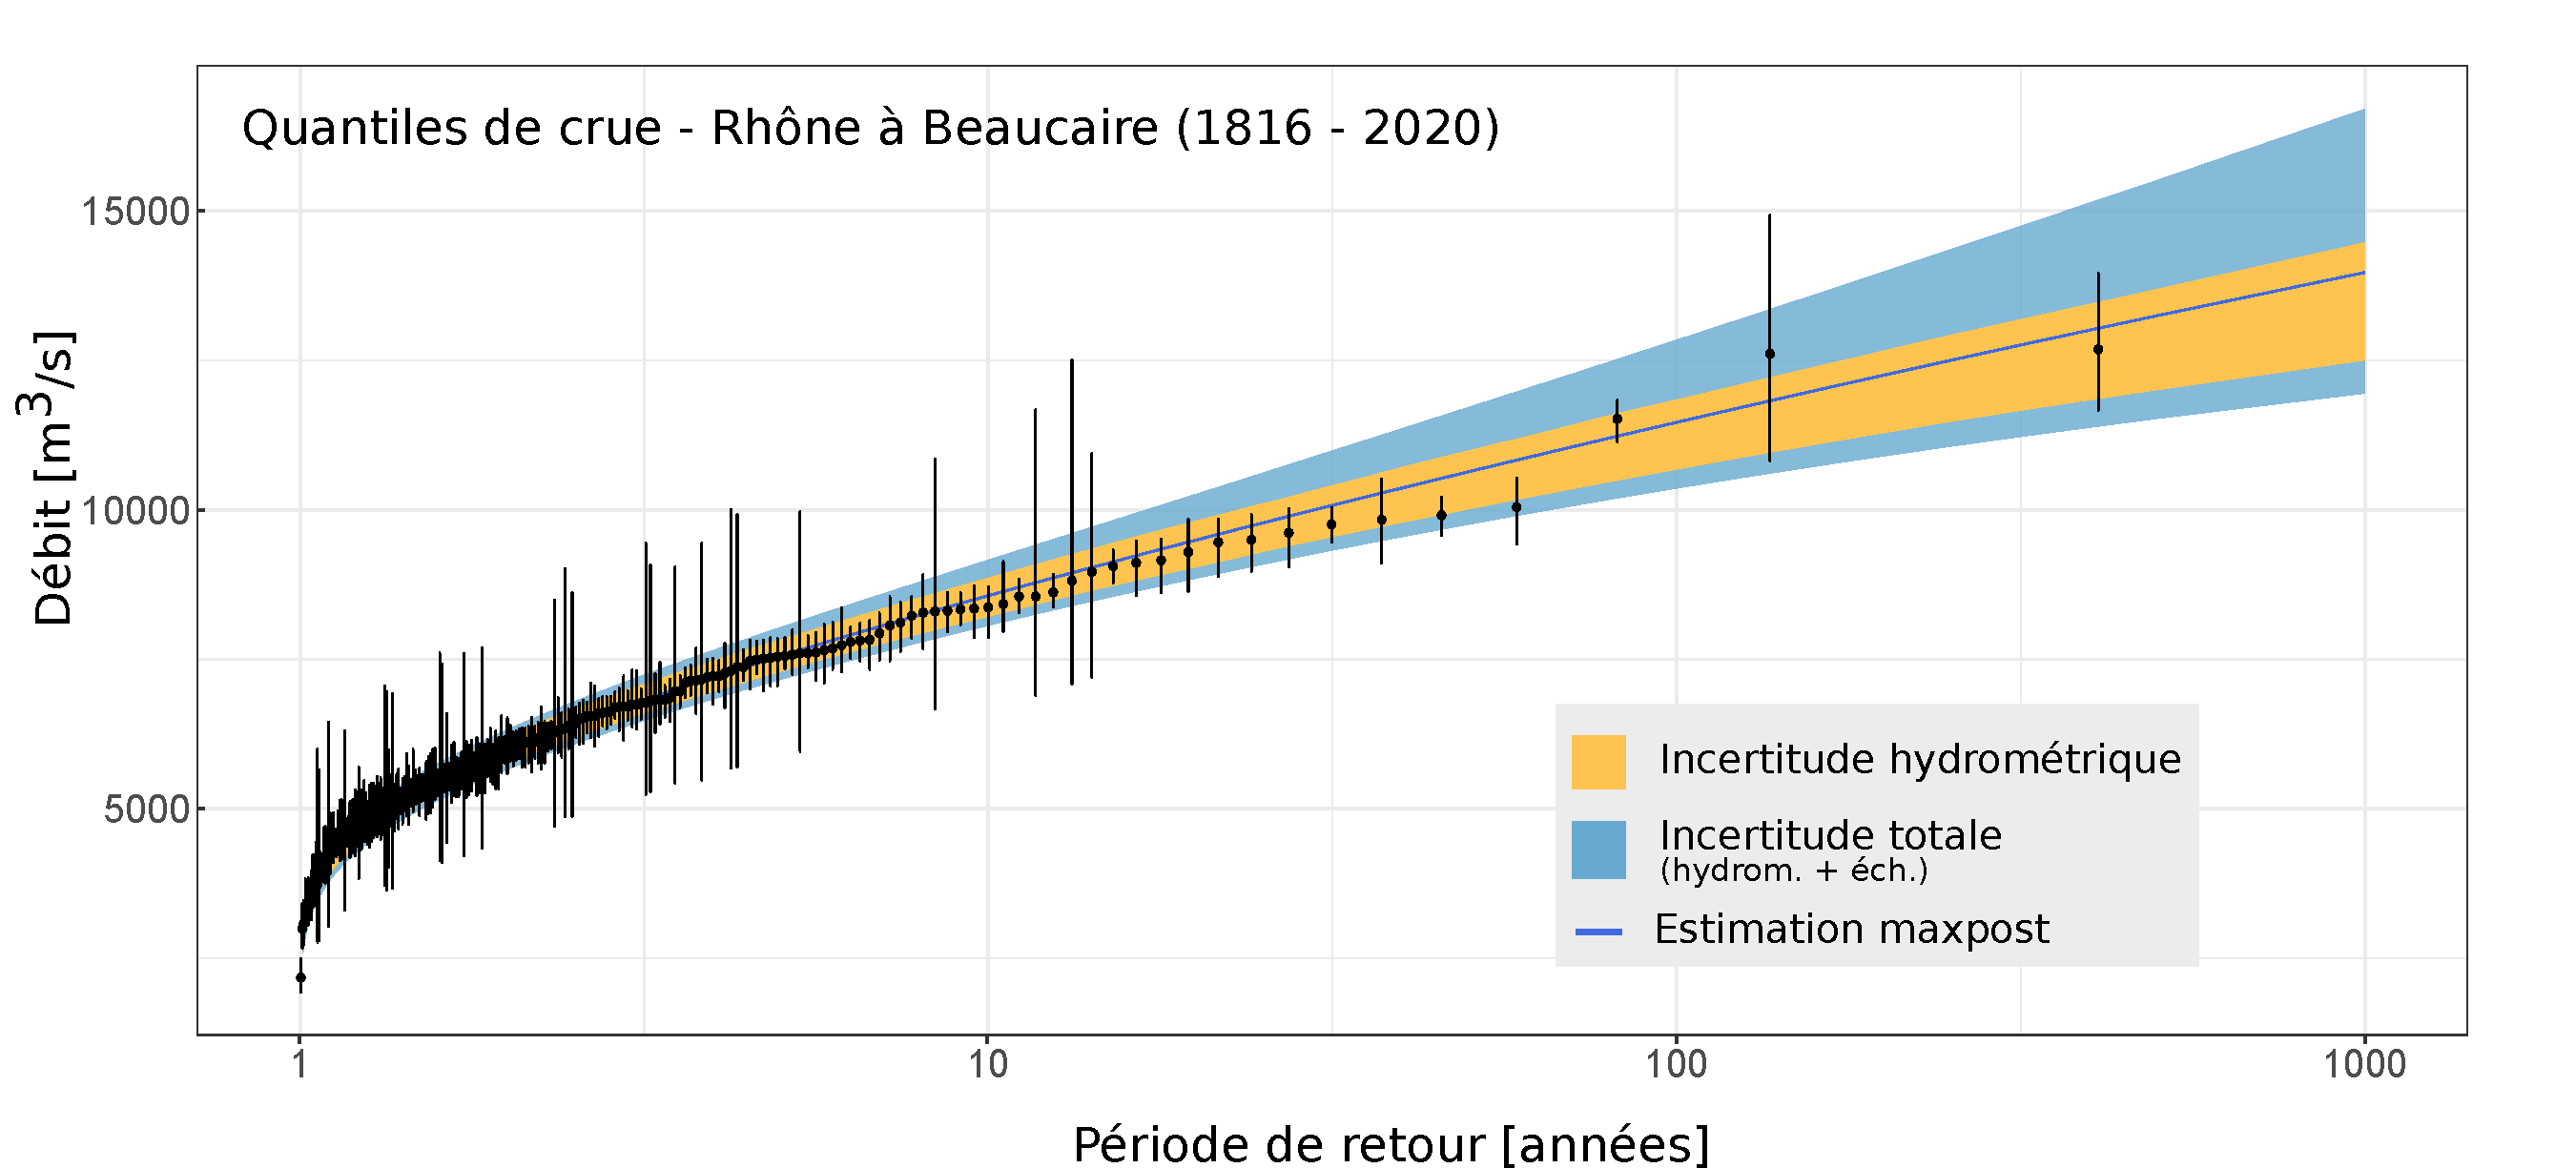
\includegraphics[width = \textwidth]{./Figures/10a-GeV_205years.pdf} 
	\end{frame}
	
	\begin{frame}[t]
		\frametitle{Analyse fréquentielle 1816-2020}
		\vfill
		\centering
		\textbf{Quelle est la part de chacune de ces deux incertitudes dans l'incertitude totale des quantiles ? }\\
		Pour des tailles de chronique variables\\
		\vfill
		\centering
		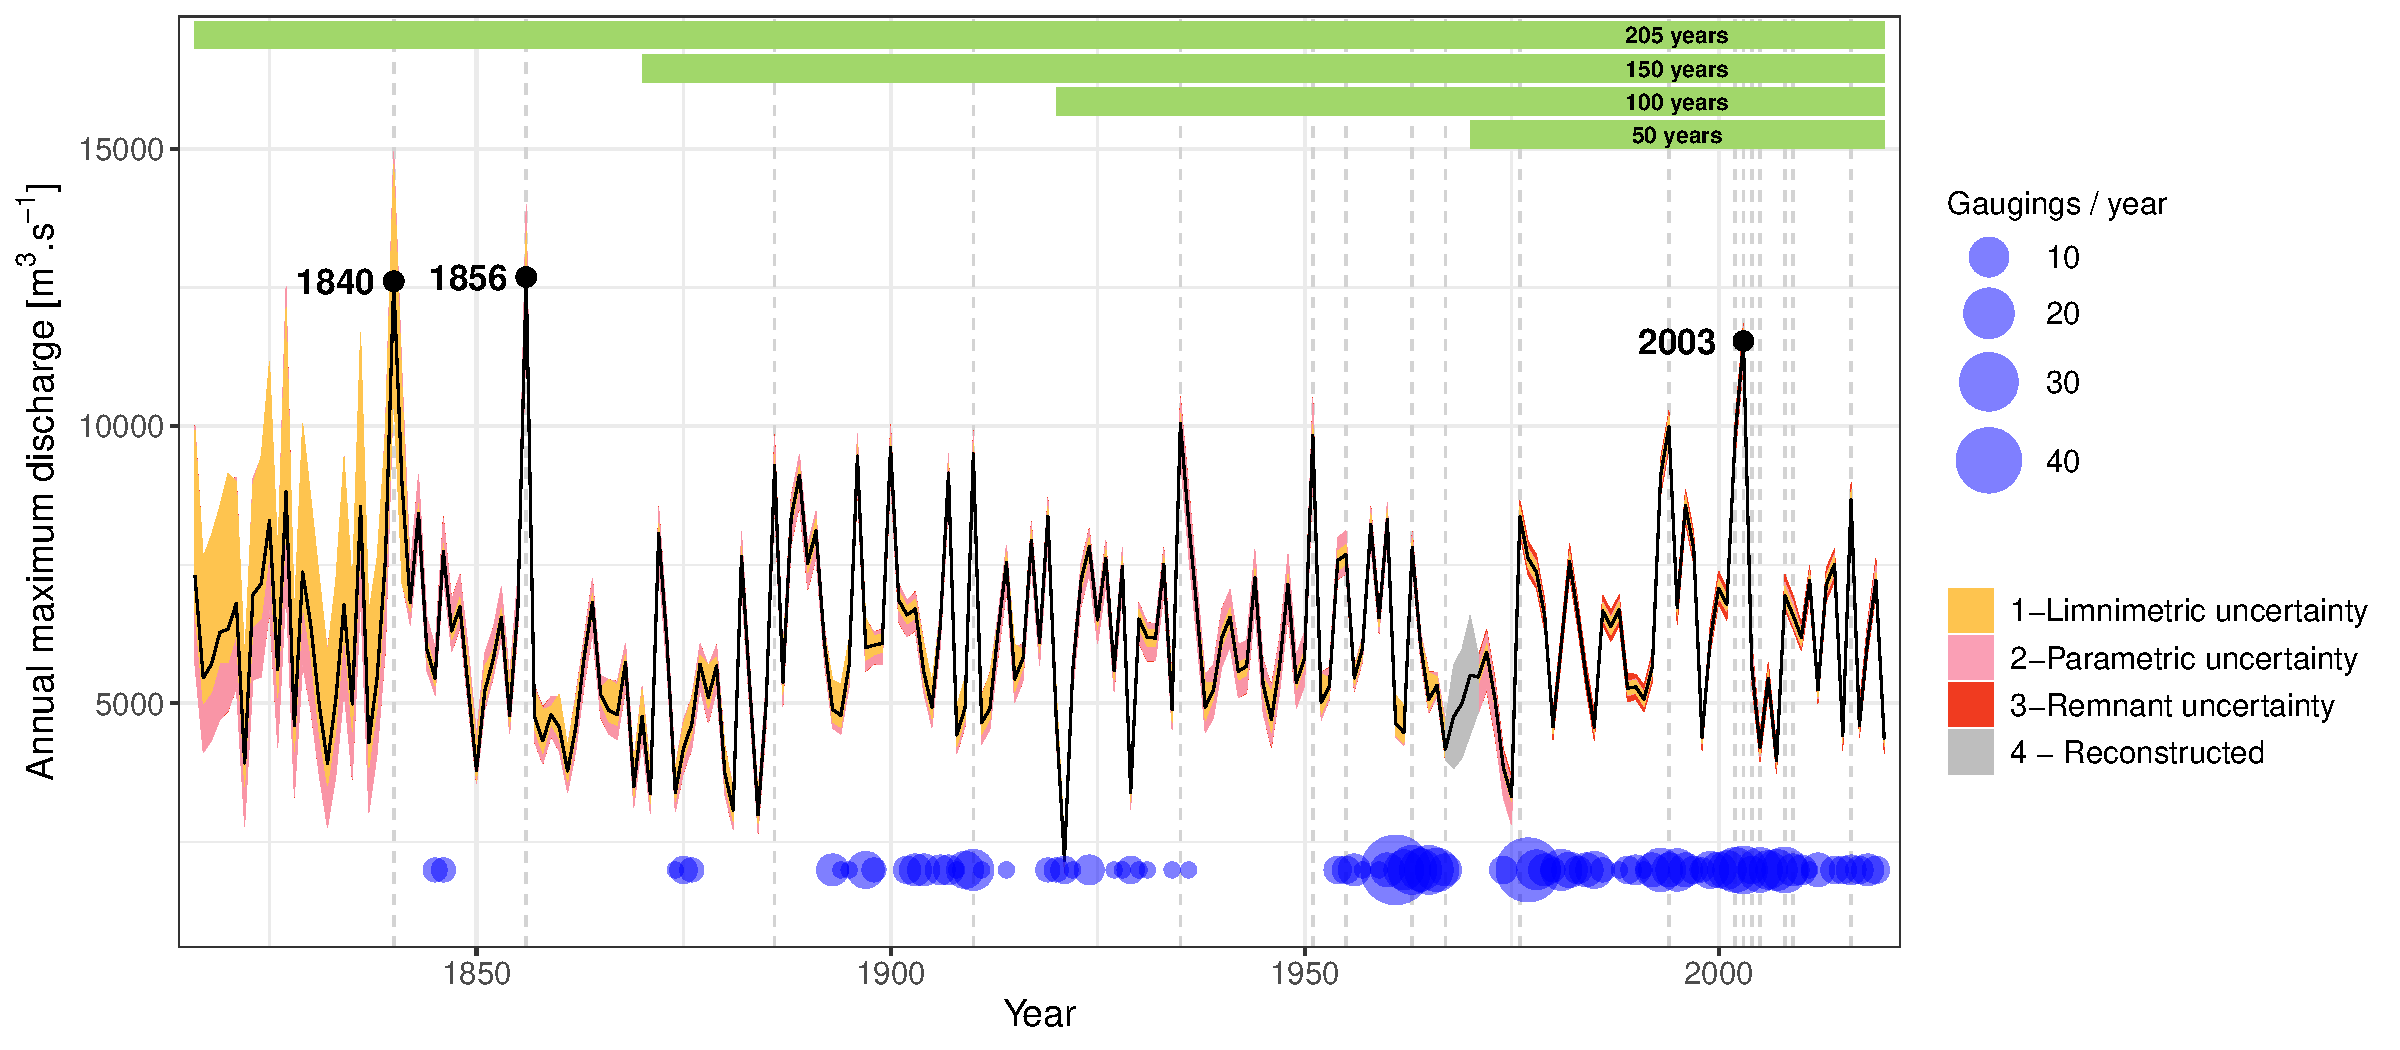
\includegraphics[width = .9\textwidth]{./Figures/IC_AMAX_Both_Bands.pdf} 
		\vfill
	\end{frame}
	
	\begin{frame}[t]
		\frametitle{Analyse fréquentielle 1816-2020}
		\vfill
		\centering
		\textbf{Quelle est la part de chacune de ces deux incertitudes dans l'incertitude totale des quantiles ? }\\
		\vfill
		\centering
		\includegraphics<1>[width = .8\textwidth]{./Figures/Ukplot4cases1.pdf}	
		\includegraphics<2>[width = .8\textwidth]{./Figures/Ukplot4cases2.pdf}	
		\vfill
	\end{frame}
	
	\begin{frame}[c]
		\frametitle{Analyse fréquentielle 1816-2020}
		\vfill
		\centering
		\textbf{Jusqu'à quelle limite l'utilisation de limnigrammes anciens permet de réduire l'incertitude des quantiles ?}
		\vfill
		\centering
		\includegraphics<1>[width = .78\textwidth]{./Figures/10e-Q1000SSize.pdf}
	\end{frame}
	
	\subsection{Conclusion partielle} 
	\begin{frame}[t]
		\frametitle{Conclusion analyse fréquentielle 1816 à 2020}
		\vfill
		\centering
		\large{\textbf{Q.2A : Quelle est la part de chacune de ces deux incertitudes dans l'incertitude totale des quantiles ?}}
		\vspace{10pt}
		\begin{itemize}
		\normalsize
			\item<2->[$\vartriangleright$] Incertitude d'échantillonnage dominante pour les grandes périodes de retour
			\vspace{5pt}
			\item<3->[$\vartriangleright$] Part relative variable selon la taille de l'échantillon
		\end{itemize}
		\vfill
	\end{frame}
	
	\begin{frame}[t]
		\frametitle{Conclusion analyse fréquentielle 1816 à 2020}
		\vfill
		\centering
		\large{\textbf{Q.2B : Jusqu'à quelle limite l'utilisation de limnigrammes anciens permet de réduire l'incertitude des quantiles ?}}
		\vspace{10pt}
		\begin{itemize}
		\normalsize
			\item<2->[$\vartriangleright$] Réduction importante de l'incertitude d'échantillonnage pour des tailles d'échantillons jusqu'à 100 ans
			\vspace{10pt}
			\item<3->[$\vartriangleright$] Au-delà de 100 ans, moindre réduction
			\vspace{10pt}
			\item<4->[$\vartriangleright$] Inclusion des crues de 1840 et 1856 $\Rightarrow$ augmentation des estimations centrales
		\end{itemize}		
	\end{frame}

\section{Analyse historique}
	\subsection{Méthode échantillon mixte}
	{
    \setbeamercolor{background canvas}{bg=myblue}
    \begin{frame}
        \begin{center}
        	\vfill
        	\textcolor{white}{\Large \textbf{Analyse fréquentielle des crues historiques (1500-2020)}}\\
		\vfill
		\textcolor{white}{\large \textbf{Comment estimer une incertitude sur le seuil de perception et la durée de la
période historique ?\\ 
		\vspace{0.5cm}
		Quel est l'apport des témoignages de crues historiques pour l'analyse fréquentielle ?
		}}
		\vfill
		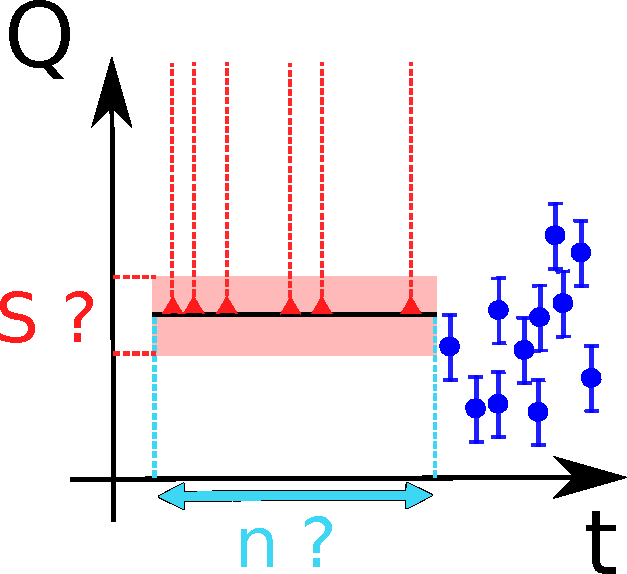
\includegraphics[width = .3\textwidth]{./Figures/uSuN.pdf}
        \end{center}
    \end{frame}
    }

	
	\begin{frame}[t]
		\frametitle{Analyse probabiliste d'un échantillon mixte}
		\begin{minipage}{0.7\textwidth}
			Échantillon mixte composé de :
			\begin{itemize}
				\item [$\vartriangleright$] Série de débits maximum annuels $\Rightarrow$ $\boldsymbol{q}= (q_t)_{t=1,...,j}$
				\vspace{5pt}
				\item<2-> [$\vartriangleright$] $k$ dépassements du seuil de perception $S$ sur $n$ années
				\item<3-> [$\vartriangleright$] Et donc : $n-k$ années sans dépassement du seuil $S$
			\end{itemize}
		\end{minipage}
%		\hfill
		\begin{minipage}{0.28\textwidth}
			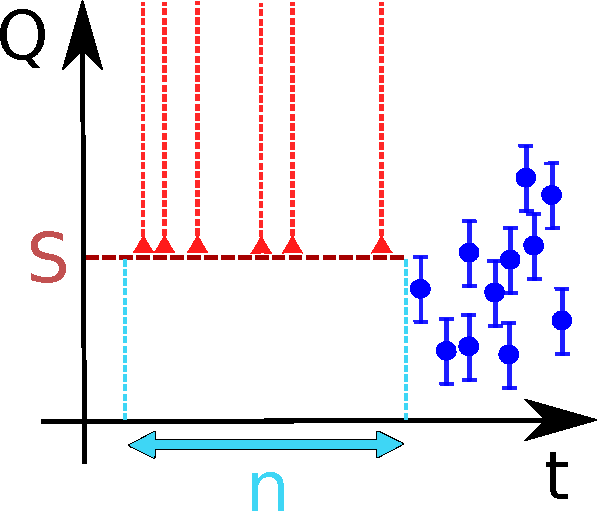
\includegraphics[width = .9\textwidth]{./Figures/Sn.pdf}
		\end{minipage}
		\vfill
		\onslide<4-> Fonction de répartition GEV : 
		\onslide<4-> \begin{equation}
			F(x;\boldsymbol{\theta}) = e^{-(1-\xi(\frac{x - \mu}{\sigma}))^{1/\xi}}
		\end{equation}
		\vfill
		\onslide<5-> La probabilité du dépassement du seuil $S$ peut alors s'écrire :	\\
		\onslide<5-> \begin{equation}
			\pi (\boldsymbol{\theta}) = \biggl( 1 - F(S;\boldsymbol{\theta})\biggl) = 1 - e^{-\biggl(1-\xi\bigl(\frac{S-\mu}{\sigma}\bigl)\biggl)^{1/\xi} }		
		\end{equation}
		\vfill
		\onslide<6-> On suppose que $k$ suit une loi binomiale de paramètres $n$ et $\pi$ $\Rightarrow$ $\mathcal{B}(n,\pi(\boldsymbol{\theta}))$
	\end{frame}		
		
	\begin{frame}[t]
		\frametitle{Analyse probabiliste d'un échantillon mixte}
		La vraisemblance de l'échantillon mixte s'écrit alors :
			\begin{equation}
			L(\boldsymbol{\theta} ; \boldsymbol{q}, k) = \underbrace{\prod_{t=1}^j f\left(q_t;\boldsymbol{\theta}\right)}_{\mathrm{période\,systématique}} \underbrace{\left\{\left(\begin{array}{l}
			n \\
			k
			\end{array}\right) F\left(S;\boldsymbol{\theta}\right)^{n-k}\left[1-F\left(S;\boldsymbol{\theta}\right)\right]^k\right\}}_{\mathrm{période\,historique}} 
			\end{equation}
			\vfill
			\onslide<2-> Formule de Bayes $\Rightarrow$ distribution des paramètres $\boldsymbol{\theta}$ sachant les données :
			\onslide<2-> \begin{equation}
				\underbrace{p(\boldsymbol{\theta} \mid \boldsymbol{q},k)}_{\mathrm{a\,posteriori}} \propto \underbrace{L(\boldsymbol{\theta};\,\boldsymbol{q},k)}_{\mathrm{Vraisemblance}} \, \underbrace{p(\boldsymbol{\theta})}_{{\mathrm{a\,priori}} }
			\end{equation}
			\vfill	
			\begin{itemize}	
			\item<3-> [$\vartriangleright$] Distribution \textit{a posteriori} explorée via une méthode MCMC \footfullcite{renard_application_2006}
			\vspace{5pt}
			\item<4-> [$\vartriangleright$] Propagation de l'incertitude hydrométrique des relevés systématiques
			\end{itemize}
	\end{frame}
	
	\subsection{4 modèles}

	\begin{frame}
	\frametitle{Données historiques et incertitudes}
		\begin{itemize}
			\item<1-> \textcolor{orange}{Modèle A} : $S$ et $n$ sont connus
			\begin{equation}
						p(\boldsymbol{\theta} \mid \boldsymbol{q},k) \propto L(\boldsymbol{\theta};\,\boldsymbol{q},k) \, p(\boldsymbol{\theta})
			\end{equation}		
			\vfill
			\item<2-> \textcolor{red}{Modèle B} : $S$ est méconnu, $n$ est connu
			\begin{equation}
						p(\boldsymbol{\theta},\textcolor{red}{S} \mid \boldsymbol{q},k) \propto L(\boldsymbol{\theta},\textcolor{red}{S};\,\boldsymbol{q},k) \, p(\boldsymbol{\theta},\textcolor{red}{S})
			\end{equation}		
			\vfill
			\item<3-> \textcolor{cyan}{Modèle C} : $S$ est connu, $n$ est méconnu
			\begin{equation}
						p(\boldsymbol{\theta},\textcolor{cyan}{n} \mid \boldsymbol{q},k) \propto L(\boldsymbol{\theta},\textcolor{cyan}{n};\,\boldsymbol{q},k) \, p(\boldsymbol{\theta},\textcolor{cyan}{n})
			\end{equation}		
			\vfill
			\item<4-> \textcolor{blue}{Modèle D} : $S$ et $n$ sont méconnus
			\begin{equation}
						p(\boldsymbol{\theta},\textcolor{blue}{S},\textcolor{blue}{n} \mid \boldsymbol{q},k) \propto L(\boldsymbol{\theta},\textcolor{blue}{S},\textcolor{blue}{n};\,\boldsymbol{q},k) \, p(\boldsymbol{\theta},\textcolor{blue}{S},\textcolor{blue}{n})
			\end{equation}		
		\end{itemize}			
	\end{frame}		

\subsection{Échantillon dégradé}
	
	\begin{frame}[c]
		\frametitle{Test des modèles proposés}
		\vfill
		Échantillon artificiellement dégradé dont les paramètres sont connus :\\
		\vspace{5pt}
		$S = 9000$ $m^3/s$ et $n = 154$ ans\\
		\vfill
		\begin{itemize}
			\item [$\vartriangleright$] Pont de Beaucaire (1816-1970) : $k$ dépassements du seuil S = 9000 m\textsuperscript{3}/s
			\vspace{5pt}			
			\item [$\vartriangleright$] Beaucaire Restitution (1971-2020) : Débits maximum annuels avec incertitude
		\end{itemize}
		\vfill
		\centering
		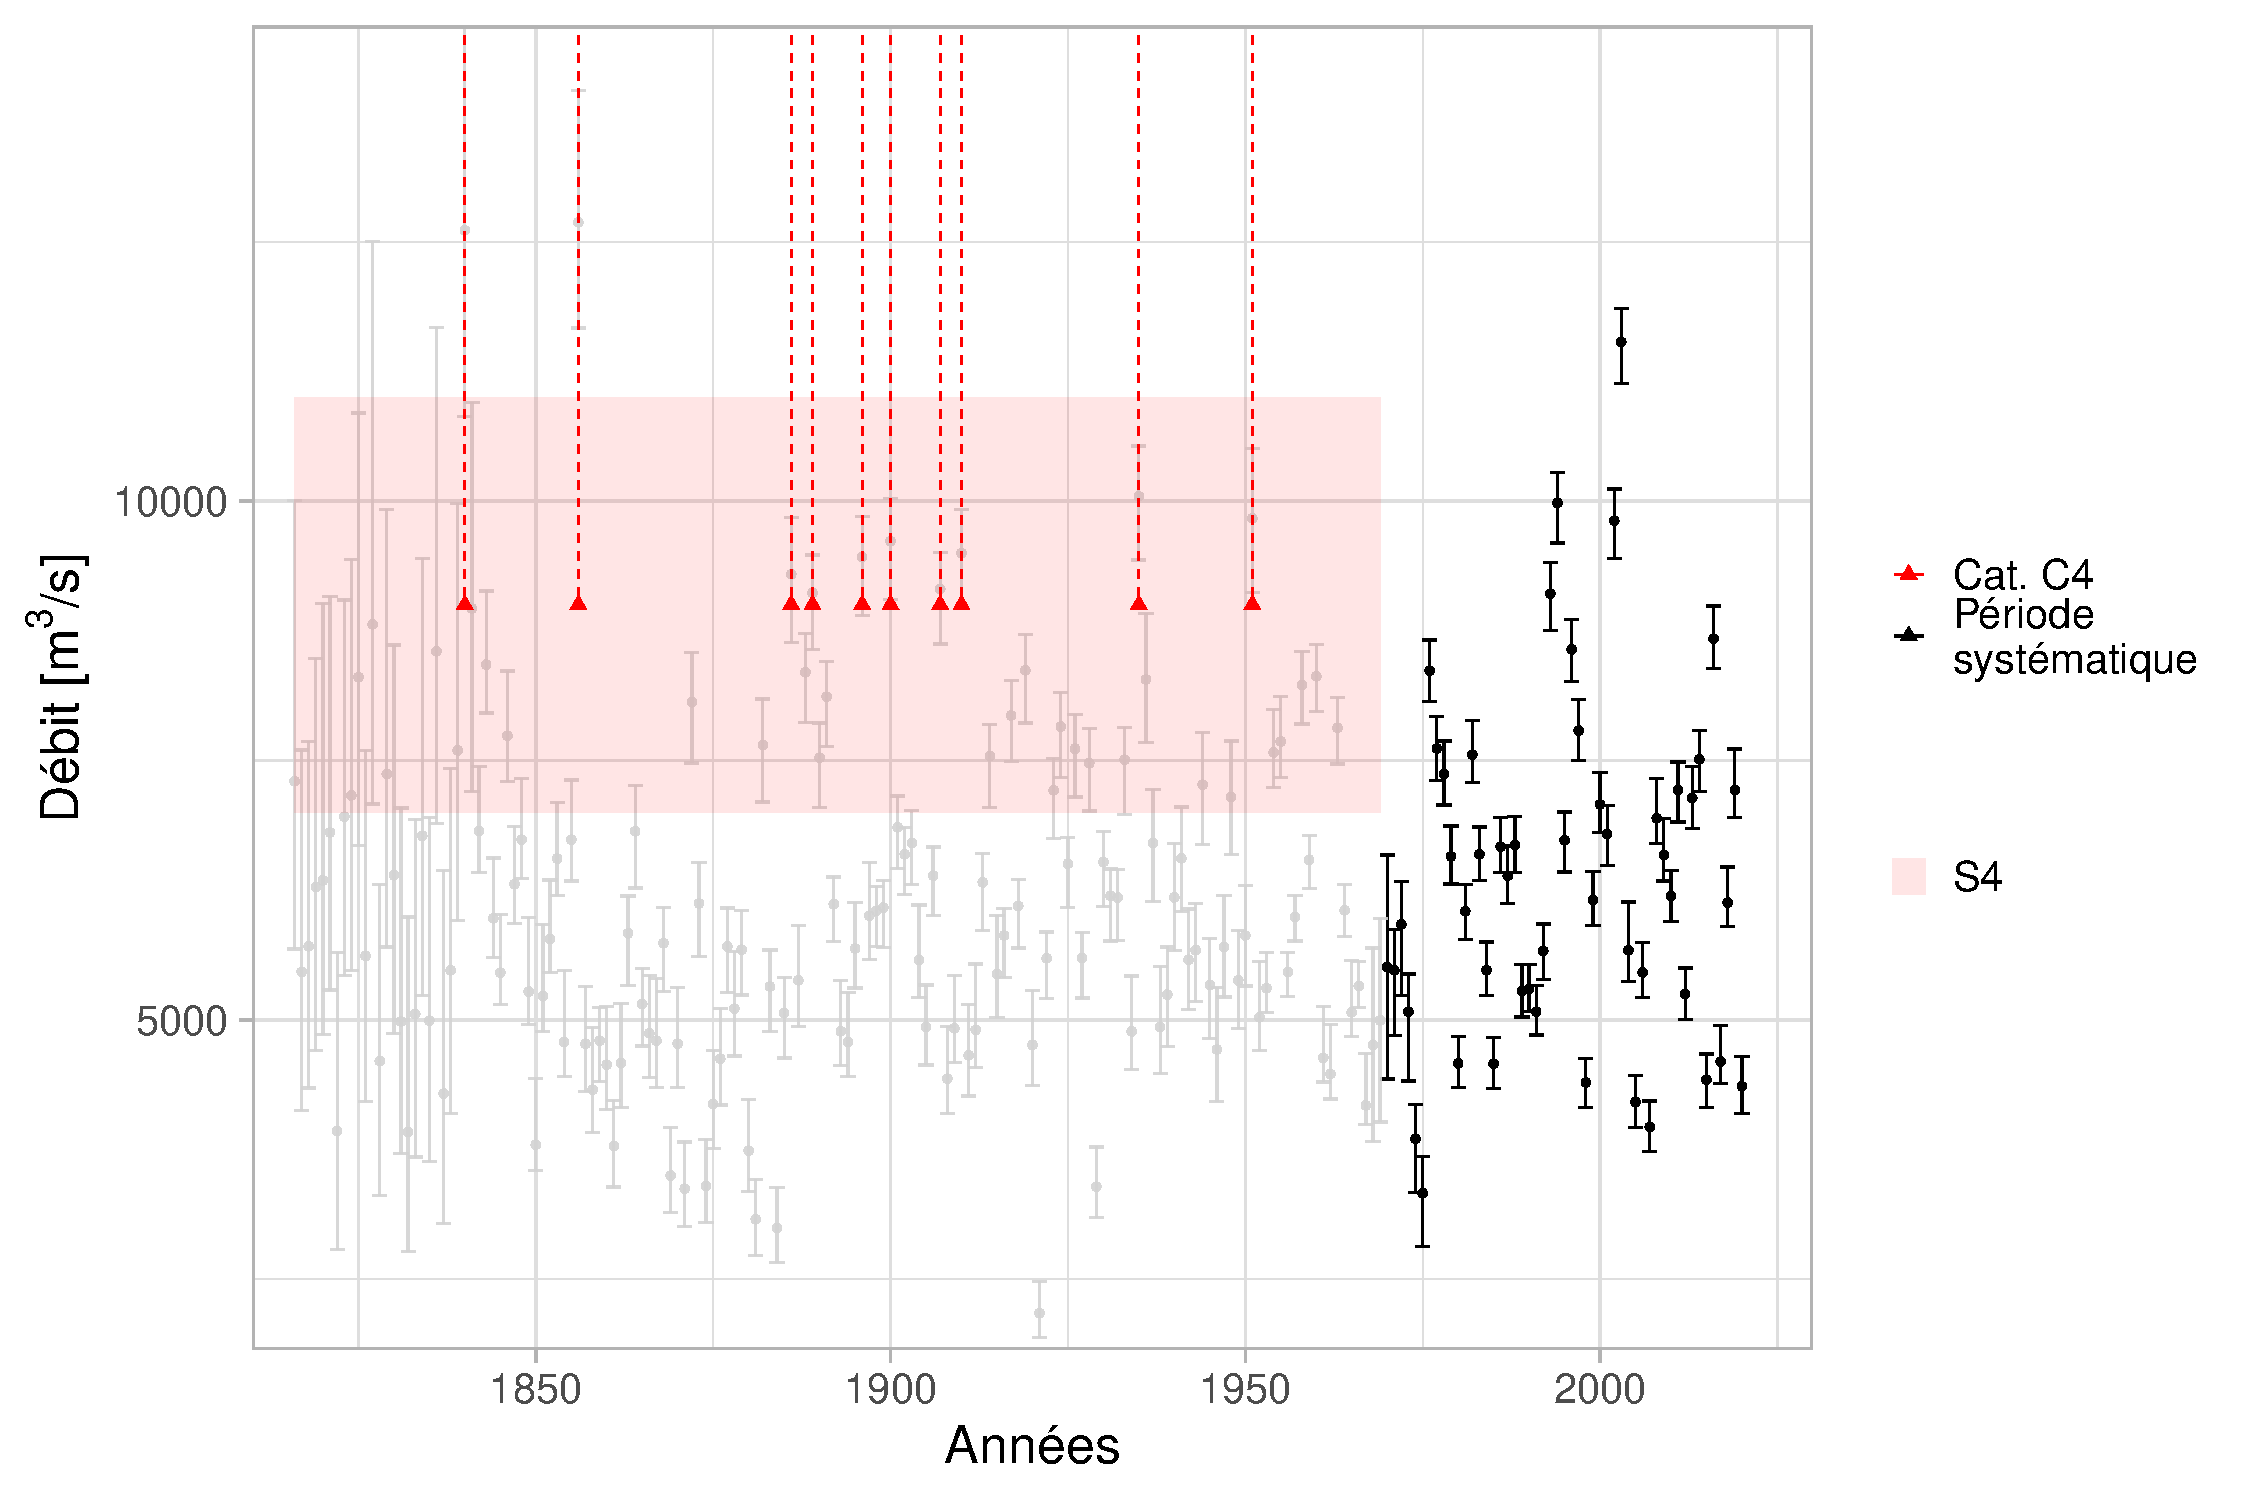
\includegraphics[width = .7\textwidth]{./Figures/EchMixteDegrad.pdf} 
		\vfill
	\end{frame}
	
	\begin{frame}[c]
		\frametitle{Test des modèles proposés}
%		\vfill
%		4 modèles $\Rightarrow$ 4 hypothèses 
%		\vfill
		Spécification d'\textit{a priori} peu informatifs :
		\begin{itemize}
			\item [$\vartriangleright$] \textbf{Seuil de perception} $S$ $\Rightarrow$ $\mathcal{N}(9000,2000)$ \\
			\vfill
			\item [$\vartriangleright$] \textbf{Date de début de la période historique} $t^*$ en 1816 $\Rightarrow \mathrm{U}(1340,1840)$ :\\
			Soit date de la première crue > $S$ - 500 ans
		\end{itemize}
		\vfill
		\begin{table}
			\centering
			\begin{tabular}{c|c|c|c|c}
	%			\hline
				Modèle & \textcolor{orange}{A} & \textcolor{red}{B} & \textcolor{cyan}{C} & \textcolor{blue}{D}\\ \hline
				Nom & u0 & uS & u$t^*$ & uS\&$t^*$ \\ \hline
				Seuil $S$ [m\textsuperscript{3}/s] & \textcolor{red}{X}  & \textcolor{green}{\checkmark} & \textcolor{red}{X}  & \textcolor{green}{\checkmark} \\ \hline
				Date $t^*$ & \textcolor{red}{X}  & \textcolor{red}{X}  & \textcolor{green}{\checkmark} & \textcolor{green}{\checkmark} \\ \hline
			\end{tabular}
		\end{table}
	\end{frame}

	
	
	\begin{frame}[c]
		\frametitle{Échantillon dégradé (1816-2020)}
		\begin{minipage}{0.38\textwidth}
		\vfill
			\begin{itemize}
				\item<1> [$\vartriangleright$] GEV série systématique 1816-2020
				\item<2> [$\vartriangleright$] GEV série systématique tronquée 1970-2020
				\item<3> [$\vartriangleright$] Modèle A : $S$ et $n$ connus
				\item<4> [$\vartriangleright$] Modèle B : $S$ méconnu et $n$ connu
				\item<5> [$\vartriangleright$] Modèle C : $S$ connu et $n$ méconnu
				\item<6> [$\vartriangleright$] Modèle D : $S$ et $n$ méconnus
			\end{itemize}
		\end{minipage}
		\hfill
		\begin{minipage}{.6\textwidth}
			\begin{center}
				\includegraphics<1>[width = \textwidth]{./Figures/BarplotArtif0.pdf} 
				\includegraphics<2>[width = \textwidth]{./Figures/BarplotArtif1.pdf} 
				\includegraphics<3>[width = \textwidth]{./Figures/BarplotArtif2.pdf} 
				\includegraphics<4>[width = \textwidth]{./Figures/BarplotArtif3.pdf} 
				\includegraphics<5>[width = \textwidth]{./Figures/BarplotArtif4.pdf} 
				\includegraphics<6>[width = \textwidth]{./Figures/BarplotArtif5.pdf} 
				\includegraphics<7>[width = \textwidth]{./Figures/BarplotArtifFull.pdf} 
			\end{center}
		\end{minipage}
	\end{frame}
	
	\begin{frame}[c]
		\frametitle{Échantillon dégradé (1816-2020)}
		\begin{minipage}{0.38\textwidth}
			\vfill
			\begin{itemize}
				\item<1-> [$\vartriangleright$] Modèle A : sous-estimation de l'incertitude
				\vspace{5pt}
				\item<2-> [$\vartriangleright$] Forte réduction de l'incertitude lorsque $S$ est connu : A et C
				\vspace{5pt}
				\item<3-> [$\vartriangleright$] Méconnaissance de $n$ peu impactante
				\vspace{5pt}
				\item<4-> [$\vartriangleright$] Valeur centrales proches de la référence (GEV 1816-2020)
			\end{itemize}
			\vfill
		\end{minipage}
		\hfill
		\begin{minipage}{.6\textwidth}
			\begin{center}
			\includegraphics<1->[width = \textwidth]{./Figures/BarplotArtifFull.pdf} 
			\end{center}
		\end{minipage}
	\end{frame}
	
	
	\begin{frame}[c]
		\frametitle{Échantillon dégradé (1816-2020)}
		\begin{minipage}{0.38\textwidth}
			\begin{itemize}
				\item<1> [$\vartriangleright$] Estimation de $S$ cohérente, en particulier pour le modèle B
				\vspace{5pt}				
				\item<2> [$\vartriangleright$] Estimation peu précise de $t^*$, en particulier modèle D\\$\Rightarrow$ \textit{a priori} plus informatifs ?
			\end{itemize}
		\end{minipage}
		\hfill
		\begin{minipage}{.6\textwidth}
			\begin{center}
			\includegraphics<1>[width = .9\textwidth]{./Figures/SArtif.pdf} 
			\includegraphics<2->[width = .9\textwidth]{./Figures/NArtif.pdf} 
			\end{center}
		\end{minipage}
	\end{frame}
	
	\subsection{Échantillon complet}
		\begin{frame}[c]
		\frametitle{Échantillon complet (1500-2020)}
		\vfill
		Échantillon mixte complet, paramètres inconnus :\\
		\vspace{5pt}
		$S = 9000$ $m^3/s$ ?? et $n = 316$ ans ?? $\Rightarrow$ \textbf{a priori} similaires au cas test\\
		\vfill
		\begin{itemize}
			\item [$\vartriangleright$] Données C4 HISTRHÔNE (de $t^*$ à 1815) : $k$ dépassements d'un seuil $S$ inconnu
			\vspace{5pt}			
			\item [$\vartriangleright$] Données systématiques : Débits maximum annuels avec incertitude (1816-2020)
		\end{itemize}
		\vfill
		\centering
		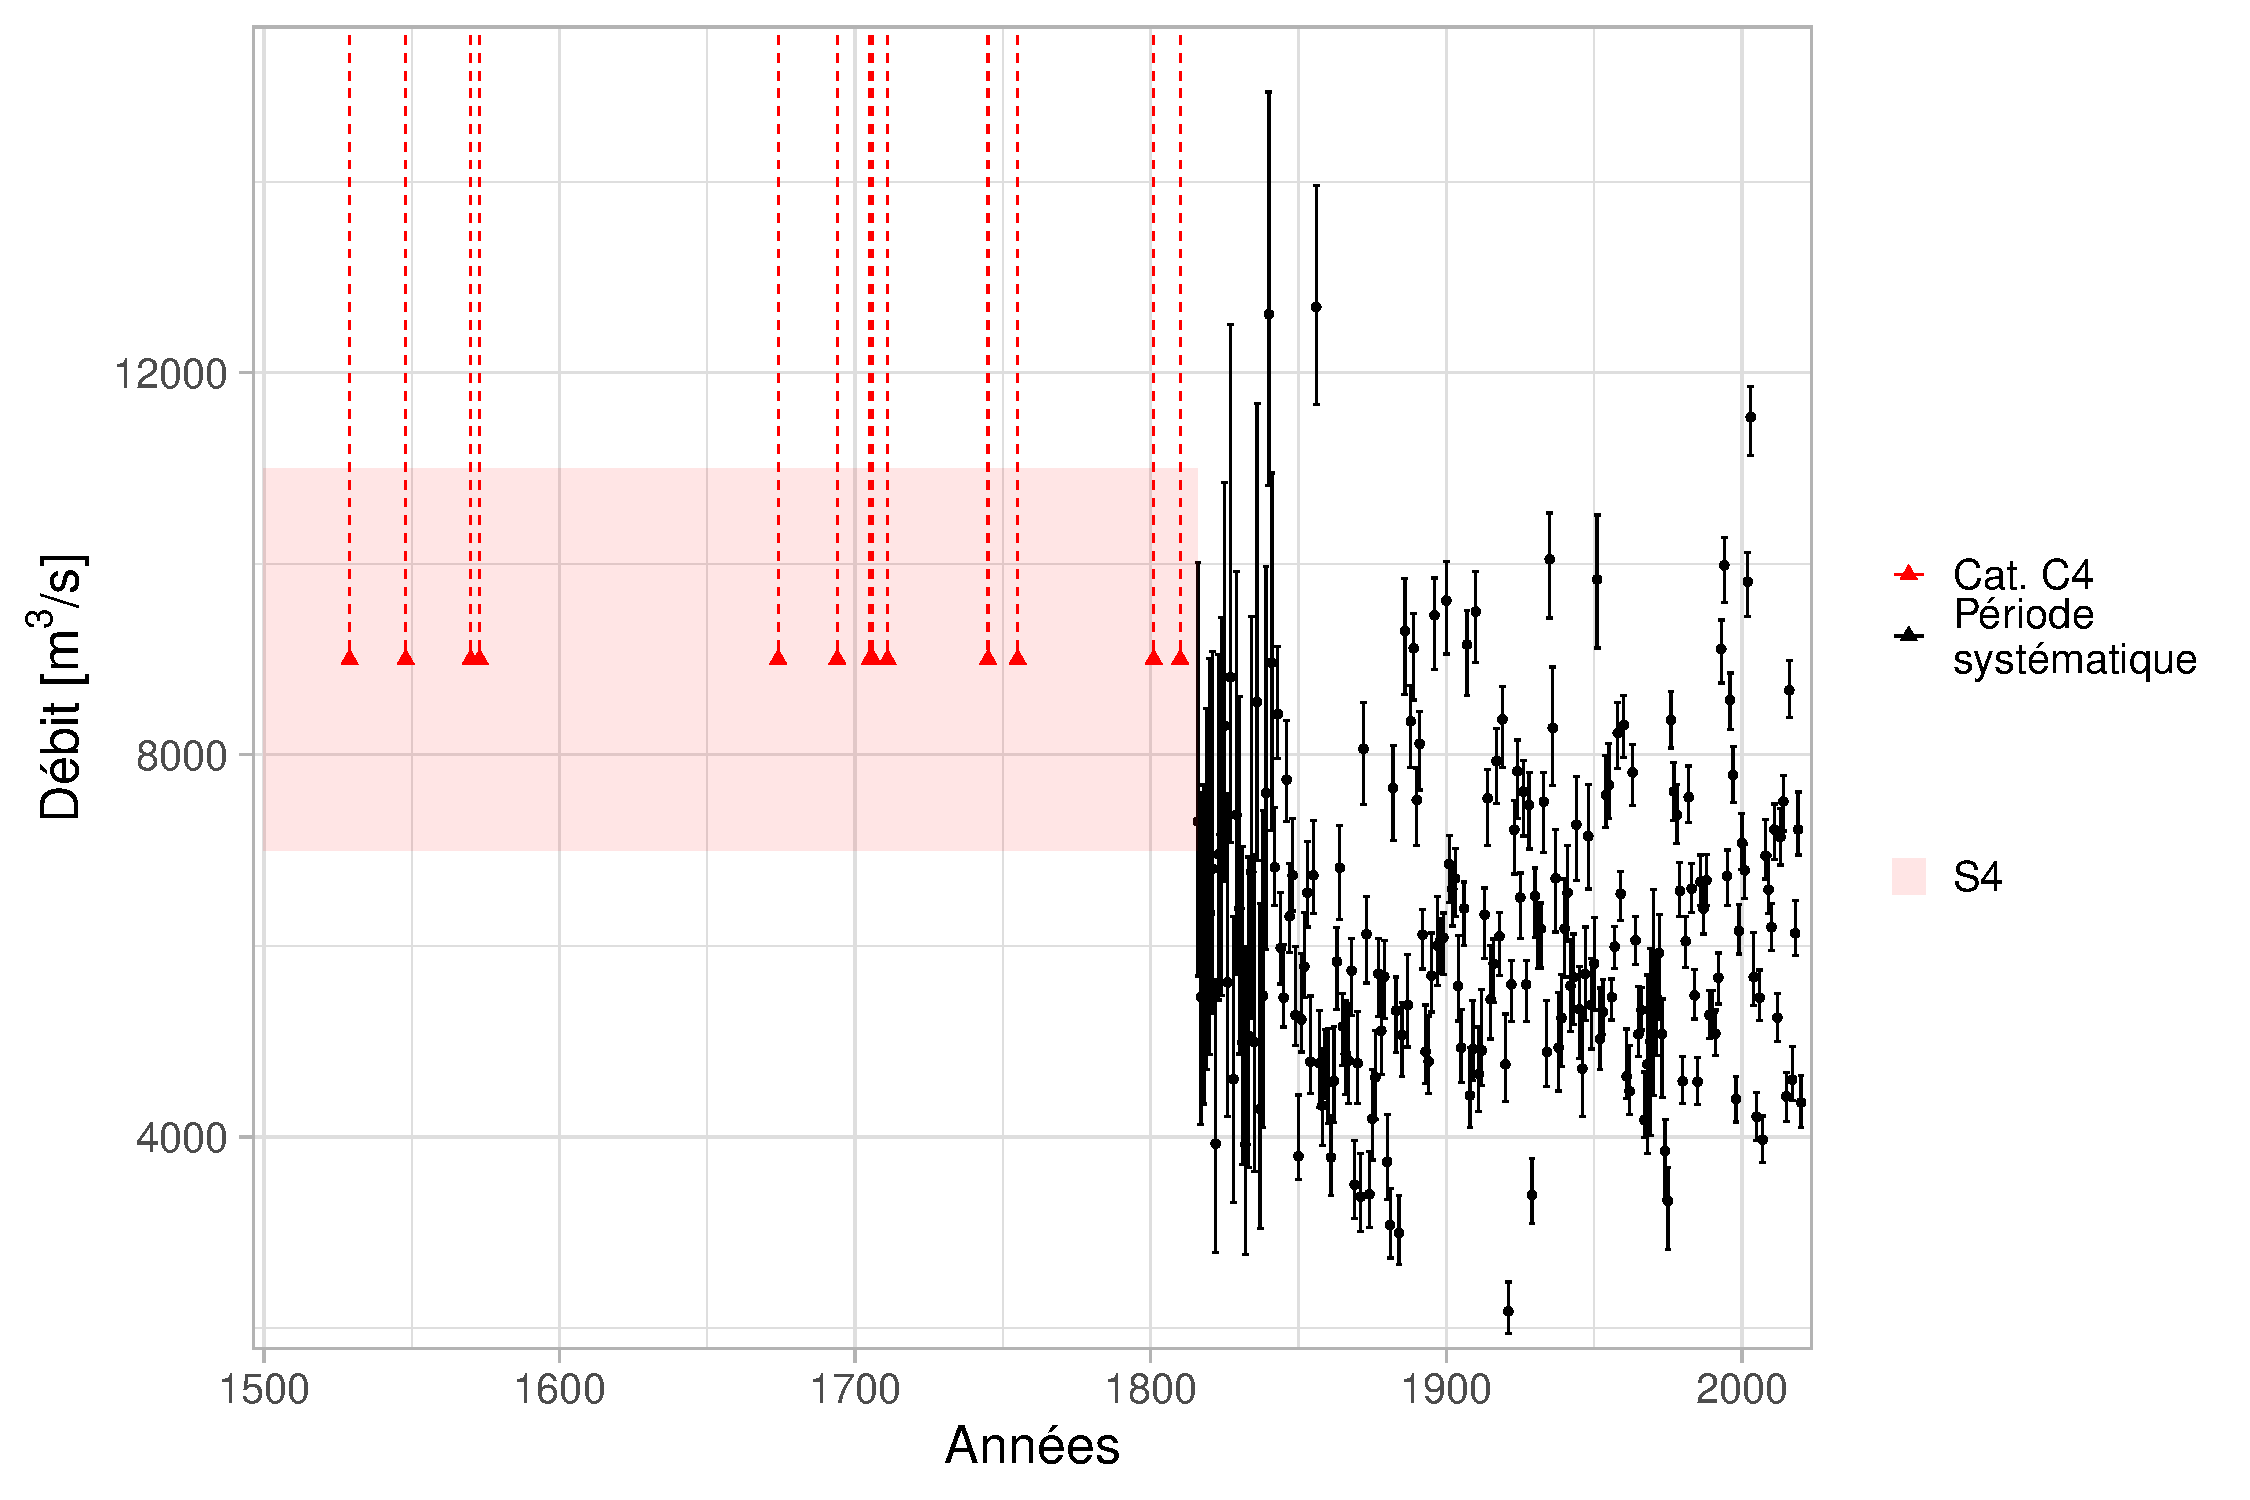
\includegraphics[width = .6\textwidth]{./Figures/EchMixteC4Bcr.pdf} 
		\vfill
	\end{frame}	
	
	
	\begin{frame}[c]
		\frametitle{Échantillon complet (1500-2020)}
		\begin{minipage}{0.39\textwidth}
			\centering
			\begin{itemize}
				\item<1-> [$\vartriangleright$] Modèle A : forte sous-estimation
				\vfill
				\item<2-> [$\vartriangleright$] Réduction d'incertitude seulement quand $S$ est connu 
				\vfill
				\item<3-> [$\vartriangleright$] Sinon, incertitude similaire à la référence
				\vfill
				\item<4-> [$\vartriangleright$] Estimations centrales légèrement plus faibles (5\%) pour A et C
			\end{itemize}
		\end{minipage}
		\begin{minipage}{0.6\textwidth}
			\begin{center}
				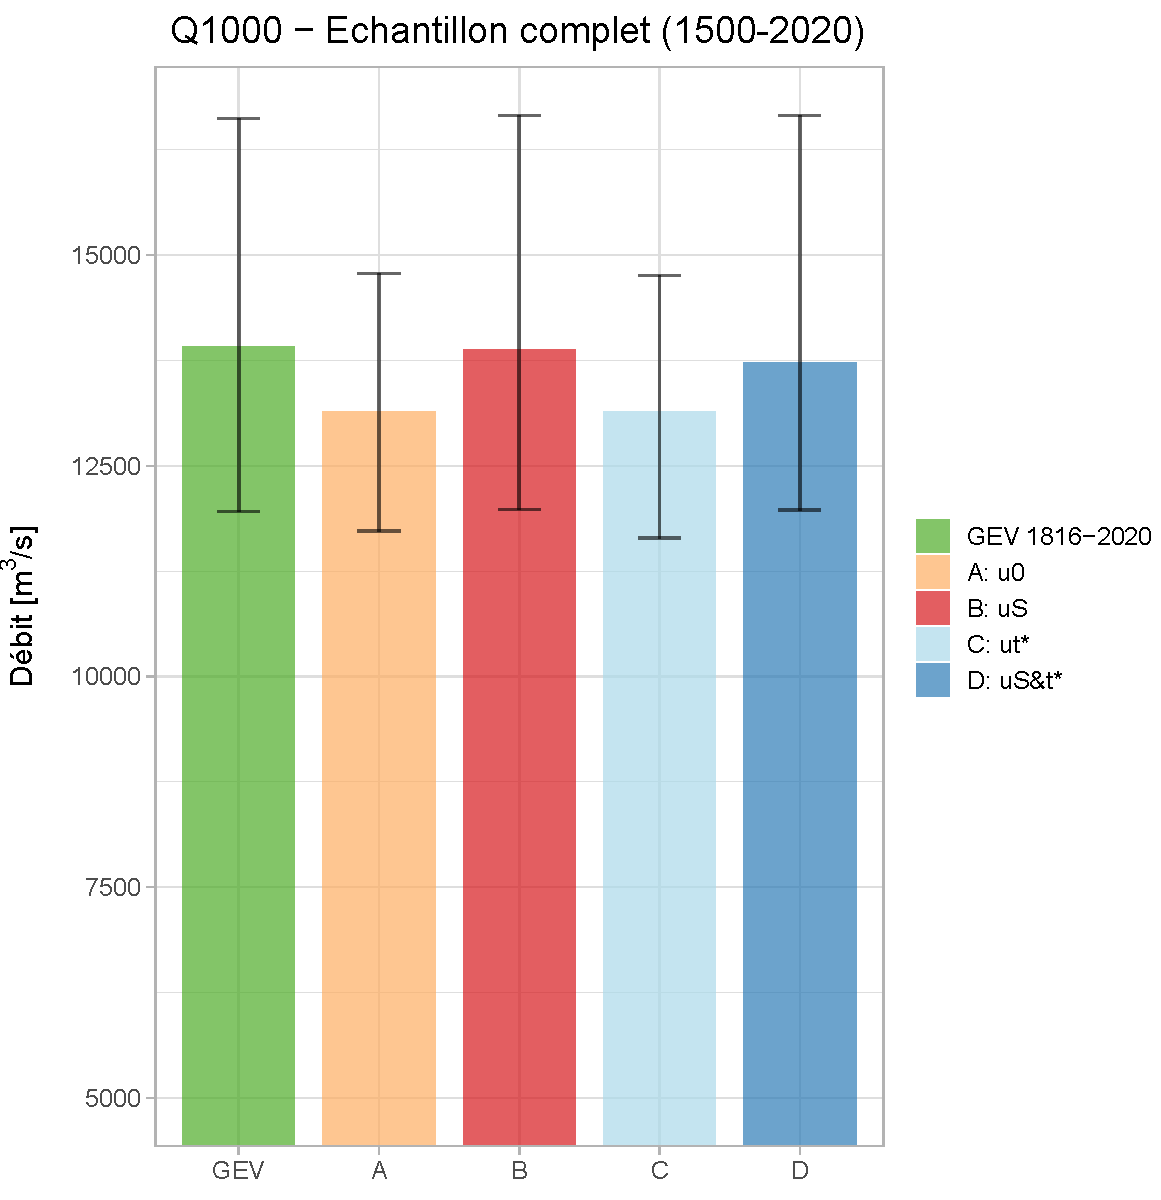
\includegraphics[width = .9\textwidth]{./Figures/BarplotC4Full.pdf} 
			\end{center}
		\end{minipage}
	\end{frame}
	
	\begin{frame}[c]
		\frametitle{Échantillon complet (1500-2020)}
		\begin{minipage}{0.39\textwidth}
			\centering
			\begin{itemize}
				\item<1-2> [$\vartriangleright$] Écart-type de $S$ réduit par rapport à l'\textit{a priori}
				\vfill
				\item<2> [$\vartriangleright$] \textit{a posteriori} de $S$ entre 9500 et 10 000 $m^3/s$
				\vfill
				\item<3-4> [$\vartriangleright$] Données moins informatives pour $n$ que pour $S$
				\vfill
				\item<4-> [$\vartriangleright$] Estimation très incertaine quand $S$ \textbf{et} $n$ sont incertains
			\end{itemize}
		\end{minipage}
		\begin{minipage}{0.6\textwidth}
			\begin{center}
				\includegraphics<1-2>[width = .9\textwidth]{./Figures/SC4.pdf} 
				\includegraphics<3->[width = .9\textwidth]{./Figures/NC4.pdf} 
			\end{center}
		\end{minipage}
	\end{frame}
	
\subsection{Conclusion analyse freq}
	\begin{frame}[c]
		\frametitle{Conclusion sur l'analyse fréquentielle de 1500 à 2020}
		\centering
		\large{\textbf{Q.3A : Comment considérer une incertitude sur le seuil de perception et la durée de la période historique ?}}\\
		\centering
			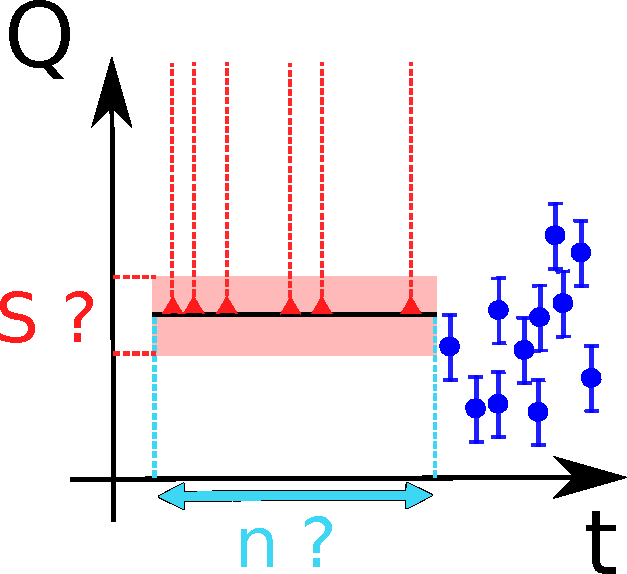
\includegraphics[width = .2\textwidth]{./Figures/uSuN.pdf} 
		\begin{itemize}
		\normalsize
			\item [$\vartriangleright$] Élaboration d'un modèle qui considère $S$ et $n$ incertains
			\vfill
			\item [$\vartriangleright$] Résultats satisfaisants sur l'échantillon test\\
		\end{itemize}
		\vfill
		\large{\textbf{Q.3B : Quel est l'apport des témoignages de crues historiques pour l'analyse fréquentielle à Beaucaire ?}}\\
		\begin{itemize}
		\normalsize
			\item [$\vartriangleright$] Réduction d'incertitude conditionnée à la connaissance de $S$
			\vfill
			\item [$\vartriangleright$] Possibilité d'utiliser des \textit{a priori} plus informatifs
			\vfill
			\item [$\vartriangleright$] Doutes sur l'exhaustivité des témoignages historiques C4 
		\end{itemize}
		\vfill
	
	\end{frame}
	
\section{Conclusion}
	\subsection{Conclusion}
	{
    \setbeamercolor{background canvas}{bg=myblue}
    \begin{frame}
        \begin{center}
        	\vfill
        	\textcolor{white}{\Large \textbf{Conclusion}}\\
		\vfill
%		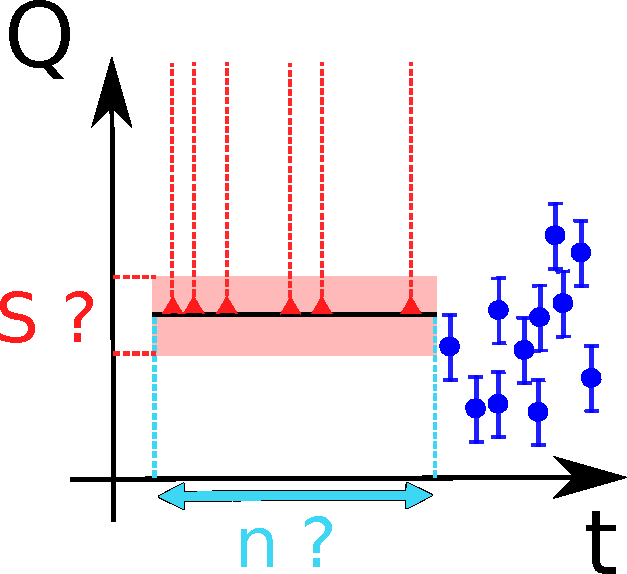
\includegraphics[width = .33\textwidth]{./Figures/uSuN.pdf}
        \end{center}
    \end{frame}
    }	
	
	%%%1
	\begin{frame}[t]
		\frametitle{Conclusion}
		\centering
		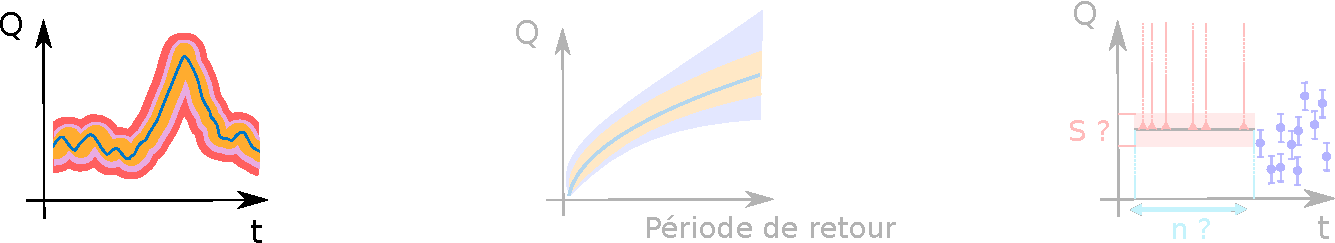
\includegraphics[width = .95\textwidth]{./Figures/SchemaConclu1.pdf} 
		\vfill
		\textbf{Comment estimer et propager les différentes sources d'incertitude hydrométrique ?}\\
		\vfill
		\begin{itemize}
			\item<1->[$\vartriangleright$] Mise au point d'une chaine de propagation complète et homogène des incertitudes 
			\vspace{5pt}
			\item<2->[$\vartriangleright$] Estimation d'hydrogrammes incertains (1816 à 2020)
			\vspace{5pt}			
			\item<3->[$\vartriangleright$] Collecte de témoignages de crues depuis 1500 et estimation de l'ordre de grandeur des crues extrêmes (Cat. C4)
		\end{itemize}
	\end{frame}
	
	%%%2
	\begin{frame}[t]
		\frametitle{Conclusion}
		\centering
		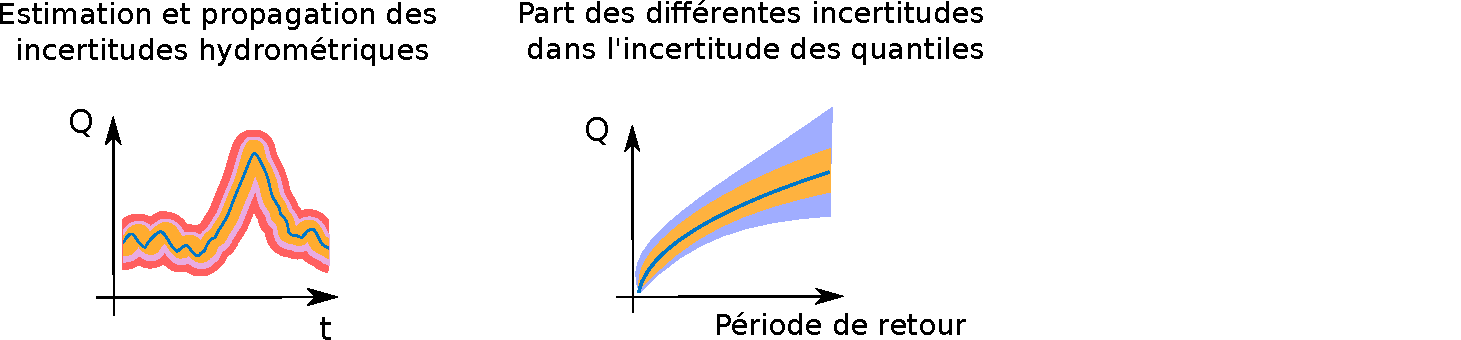
\includegraphics[width = .95\textwidth]{./Figures/SchemaConclu2.pdf} 
		\vfill
		\textbf{Quelle est la part relative des deux sources d'incertitudes dans l'incertitude totale des
quantiles ?}\\
\vspace{5pt}
		\textbf{Jusqu'à quelle limite l'utilisation de limnigrammes anciens permet de réduire l'incertitude des quantiles ?}\\
		\vfill
		\begin{itemize}
			\item<1->[$\vartriangleright$] Incertitude d'échantillonnage dominante pour les grandes périodes de retour
			\vspace{5pt}
			\item<2->[$\vartriangleright$] Part relative variable selon la taille de l'échantillon
			\vspace{5pt}
			\item<3->[$\vartriangleright$] Réduction importante de l'incertitude d'échantillonnage jusqu'à des tailles d'échantillon de 100 ans
			\vspace{5pt}
			\item<4->[$\vartriangleright$] Estimations centrales supérieures après inclusion de 1840 et 1856
		\end{itemize}
	\end{frame}
	
		
	%%%%3
		\begin{frame}[t]
		\frametitle{Conclusion}
		\centering
		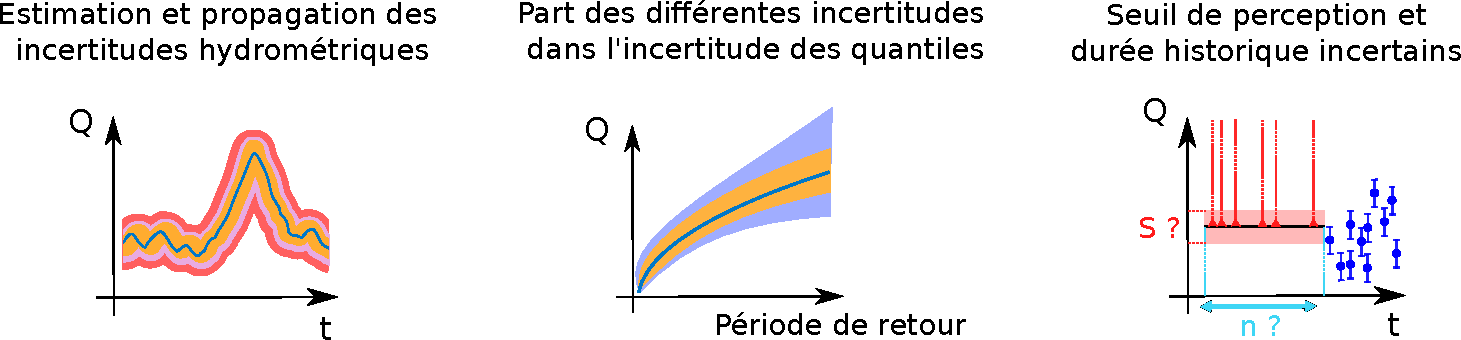
\includegraphics[width = .95\textwidth]{./Figures/SchemaConclu3.pdf} 
		\vfill
		\textbf{Comment prendre en compte l'incertitude autour de $S$ et $n$ ?}\\
		\vspace{5pt}
		\textbf{Quel est l'apport des témoignages historiques de crues pour l'analyse fréquentielle?}\\
		\vfill
		\begin{itemize}
			\item<1->[$\vartriangleright$] Construction d'un modèle fréquentiel pour lequel $S$ et/ou $n$ sont incertains
			\item<2->[$\vartriangleright$] Résultats satisfaisants sur échantillon test
			\item<3->[$\vartriangleright$] Réduction d'incertitude conditionnée à la connaissance de $S$ pour l'échantillon complet
			\item<4->[$\vartriangleright$] Forte incertitude lorsque $S$ et $n$ sont incertains
		\end{itemize}
	\end{frame}

	\subsection{Perspectives Beaucaire}
	\begin{frame}
		\frametitle{Perspectives à Beaucaire}
		\begin{minipage}{0.6\textwidth}
			\vfill		
			\begin{itemize}
				\item<1->[$\vartriangleright$] Utilisation de données historiques complémentaires\footfullcite{fanget_historical_2013}\\
				\vfill		
				\item<2->[$\vartriangleright$] Prise en compte de la variabilité climatique : impact non-homogène sur le bassin versant \footfullcite{leblois_evaluation_2002} \footfullcite{giuntoli_floods_2019}\\
				\vfill
				\item<3->[$\vartriangleright$] Analyse distribuée pour chaque sous-bassin versant avec utilisation de données historiques\\
				\vfill
				\item<4->[$\vartriangleright$] Analyse conditionnelle au type de temps/type de crue : océanique, méditerranéenne...\\
				\vfill
				\item<5->[$\vartriangleright$] Étude de la variabilité hydroclimatique sur 5 siècles \footfullcite{bloschl_current_2020}		\\
			\end{itemize}
		\end{minipage}
		\begin{minipage}{0.39\textwidth}
			\begin{center}
				\includegraphics<1>[width = .45\textwidth]{./Figures/Sedim.pdf} 
				\includegraphics<2>[width = .95\textwidth]{./Figures/NAO.png} 
				\includegraphics<4>[width = .4\textwidth]{./Figures/TypeTemps.png} 
				\includegraphics<5>[width = \textwidth]{./Figures/Bloeshl.png}
			\end{center}
		\end{minipage}
	\end{frame}
	
	\subsection{Perspectives générales}
	\begin{frame}
		\frametitle{Perspectives générales}
		\vfill
		\begin{itemize}
			\item<1->[$\vartriangleright$] Utilité des nombreuses données hydroclimatiques qui dorment dans les archives
			\vfill
			\item<2->[$\vartriangleright$] Test du modèle sur d'autres stations/types de données
			\vfill
			\item<3->[$\vartriangleright$] Sensibilisation collective aux risques naturels : \\ \og \textit{La nouvelle génération s'était habituée à la mansuétude, à la bénignité du Rhône, lorsque tout à coup, les eaux montèrent à une hauteur inusitée} \fg{}. \textbf{A. Eyssette, 1789}
				\end{itemize}
	\end{frame}
	
	\subsection{Hommage G Pichard}
	\begin{frame}
		\frametitle{Hommage à Georges PICHARD}
		\centering
		\og \textit{Nous avons pu assister nous-mêmes à cette mise à l'écart et cet oubli, volontaire ou pas, se soldant par la \textbf{perte par inondation} - ironie de l'histoire - des données rassemblées par des générations d'observateurs antérieurs pour permettre} [...] \textit{la prévision des inondations catastrophiques} \fg{} \footfullcite{pichard_sept_2014}
	\end{frame}
	
	{
    \setbeamercolor{background canvas}{bg=myblue}
    \begin{frame}
        \begin{center}
        	\vfill
        	\textcolor{white}{\Large \textbf{Merci pour votre attention !}}\\
		\vfill
%		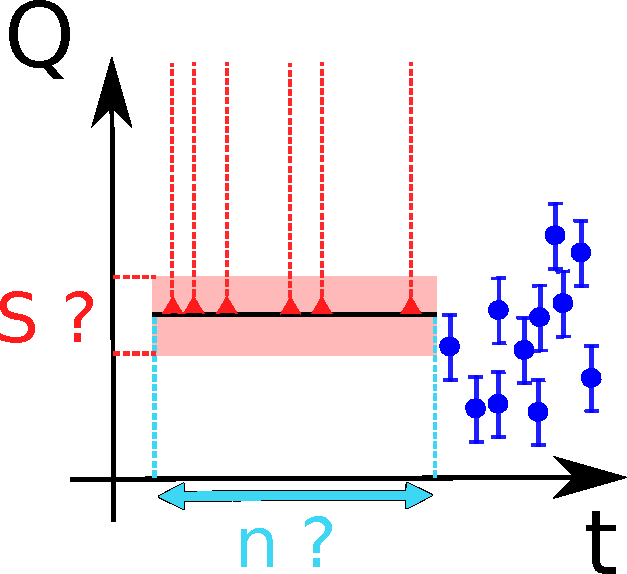
\includegraphics[width = .33\textwidth]{./Figures/uSuN.pdf}
        \end{center}
    \end{frame}
    }	
    



	\appendix



%\section{Annexes}	

%% BONUS SLIDES
%%%%%%%%% 4 %%%%%%%%%    Théorie des valeurs extrêmes
	\begin{frame}%[c]
		\frametitle{Théorie des valeurs extrêmes}
		\vfill
		\textbf{La théorie des valeurs extrêmes} nous donne le cadre pour modéliser ces processus \footfullcite{fisher_limiting_1928}\textsuperscript{;}\footfullcite{gumbel_statistics_1958}
		\vfill
		\begin{itemize}
			\item<2-> [$\vartriangleright$] On a $X_1,...,X_n$ une séquence de \textbf{variables aléatoires} $iid$\\
			\textit{Par exemple une série temporelle de débits}
			\vspace{5pt}
			\item<3-> [$\vartriangleright$] La \textbf{valeur maximale sur un bloc} de $n$ valeurs est $M_n = max(X_1,...,X_n)$\\ \textit{Par exemple une série de maximum annuels de débit}
			\vspace{5pt}
			\item<4> [$\vartriangleright$] La distribution de $M_n$ quand $n\rightarrow \infty$ converge vers la loi généralisée des valeurs extrêmes : $GEV(\mu,\sigma,\xi)$

		\end{itemize}	
	\end{frame}
	
	%%%%%%%%% 11 %%%%%%%%%	
	\begin{frame}
    	\frametitle{Estimation des courbes de tarage}
    		Équation de la courbe de tarage pour un lit simple : 
    		\begin{equation}
    			Q = \textcolor{red}{a}(h-b)^{\textcolor{red}c}
    		\end{equation}
    		Où Q est le débit, h la hauteur d'eau, b la cote du fond du chenal \\
		\vspace{1cm}
		Peut être approchée par diverses formules hydrauliques :
		\vfill
		\begin{minipage}{.4\textwidth}
			\begin{itemize}
				\item<2->[$\vartriangleright$] Contrôle par chenal rectangulaire : Manning-Strickler\\
				\vspace{0.5cm}
				\item<3->[$\vartriangleright$] Contrôle par seuil rectangulaire : loi de seuil
			\end{itemize}
		\end{minipage}
		\begin{minipage}{.55\textwidth}
			\begin{center}
%				
%				\vspace{5pt}
				\onslide<2-> $Q = \underbrace{Ks\sqrt{S}Bc}_{\mathrm{\textcolor{red}{a}}}(h-b)\underbrace{^{5/3}}_{\mathrm{\textcolor{red}{c}}}$\\
				\vspace{0.5cm}
				\onslide<3-> $Q = \underbrace{C_r\sqrt{2g}B_w}_{\mathrm{\textcolor{red}{a}}}(h-b)\underbrace{^{1.5}}_{\mathrm{\textcolor{red}{c}}}$
			\end{center}
		\end{minipage}
    \end{frame}
    
    \begin{frame}
    	\frametitle{Estimation des courbes de tarage}
    		\vfill
    		Analyse hydraulique des différents contrôles successifs ou additifs
    		\vfill
    		\begin{minipage}{.49\textwidth}
    			\begin{itemize}
    				\item<1->[$\vartriangleright$] Contrôles par seuils (radiers)
    				\vspace{0.5cm}
    				\item<1->[$\vartriangleright$] Contrôles par chenal (lit majeur)
    			\end{itemize}
    		\end{minipage}
    		\begin{minipage}{.49\textwidth}
    			\centering
    			\includegraphics<1->[width = .9\textwidth]{./Figures/Controles.jpg} 
    		\end{minipage}
    		\vfill
    		Équation pour $Nseg$ segments et $Nc$ contrôles hydrauliques
    		\centering
    		\begin{equation}
    			Q =\sum_{i=1}^{N_{\mathrm{seg}}}\left(1_{\left[\kappa_{i-1} ; \kappa_i[\right.}(h) \sum_{j=1}^{N_{\mathrm{c}}} \mathcal{M}(i, j) a_j\left(h-b_j\right)^{c_j}\right)   		 		
    		\end{equation}
    \end{frame}
      
    %%%%%%%%% 12 %%%%%%%%%	
	\begin{frame}
    	\frametitle{Estimation des courbes de tarage}
	Estimation bayésienne des paramètres de la courbe de tarage : \textbf{BaRatin}\footfullcite{le_coz_combining_2014}\\
		\vfill
		\begin{center}
			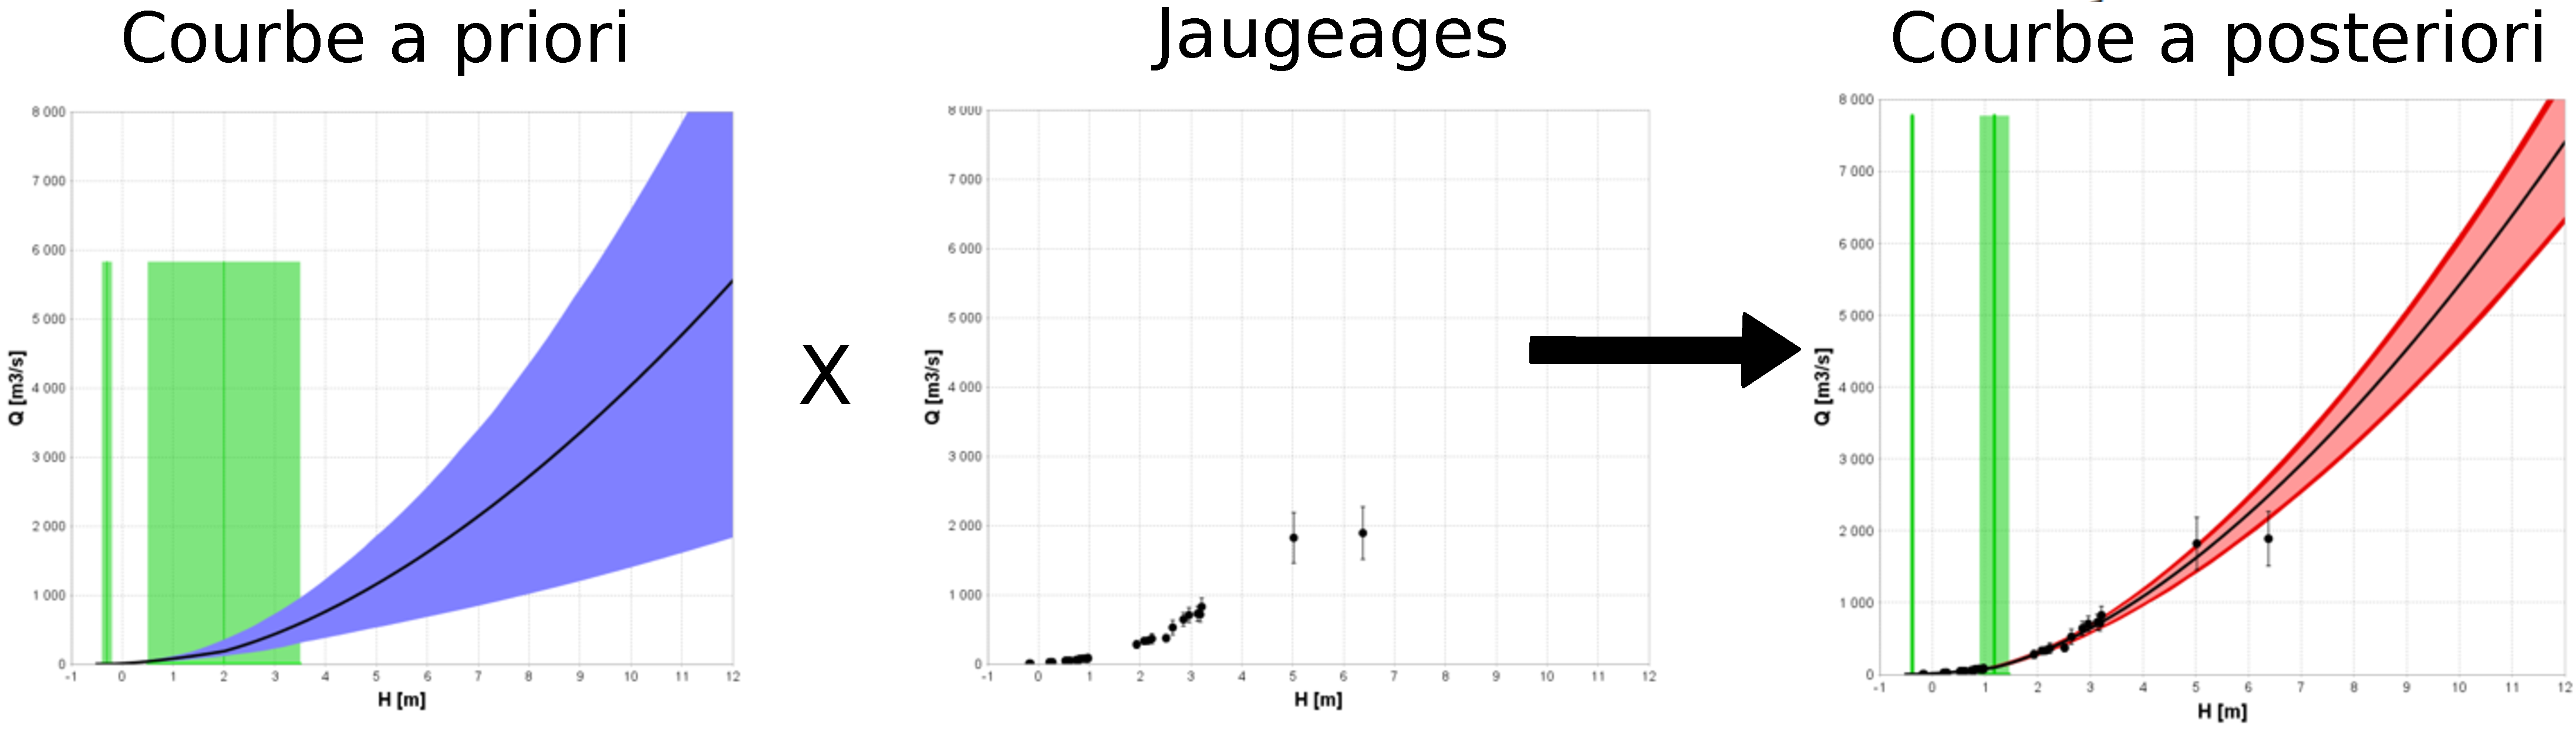
\includegraphics[width = .8\textwidth]{./Figures/Baratin.pdf} 
		\end{center}
	\begin{itemize}
			\item<1->[$\vartriangleright$] Courbe \textbf{\textit{a priori}} $\rightarrow$ connaissance hydraulique de la station\\		
			\vspace{5pt}
			\item<2->[$\vartriangleright$] Courbe \textbf{\textit{a posteriori}} $\rightarrow$ combinaison courbe \textbf{\textit{a priori}} jaugeages incertains \\		
	\end{itemize}		
			\vspace{5pt}
			\centering
			\onslide<3->$\underbrace{p(\theta,\sigma_f | \tilde{Q},\tilde{H})}_{posterior} \propto \underbrace{p(\tilde{Q}|\theta,\sigma_f,\tilde{H})}_{vraisemblance} \, \underbrace{p(\theta,\sigma_f)}_{prior}$
		
%		\begin{minipage}{.4\textwidth}
			
%		\end{minipage}
%		\begin{minipage}{.55\textwidth}
%			\begin{center}
%				\includegraphics<2>[width = \textwidth]{./Figures/Baratin.pdf} 
%			\end{center}
%		\end{minipage}
	\end{frame}

%	\subsubsection{Détarages}
	%%%%%%%%% 12 %%%%%%%%%
	\begin{frame}%[c]
		\frametitle{Détarages}
		Ruptures dans la relation hauteur/débit\\
		\vspace{15pt}
		\begin{center}
			\includegraphics<1>[width = .45\textwidth]{./Figures/Detar1.pdf} 
			\includegraphics<2>[width = .45\textwidth]{./Figures/Detar2.pdf} 
%			\includegraphics<3>[width = .45\textwidth]{./Figures/Detar3.pdf} 
		\end{center}
	\end{frame}
	
	%%%%%%%%% 11 %%%%%%%%%
	\begin{frame}%[c]
		\frametitle{Segmentation des jaugeages}
		Méthode bayésienne de détection des détarages \footfullcite{darienzo_detection_2021}\\
		\vspace{10pt}
		\begin{center}
			\includegraphics<1>[width = .3\textwidth]{./Figures/CT1.pdf} 
			\includegraphics<2>[width = .3\textwidth]{./Figures/CT2.pdf} 
			\includegraphics<3>[width = .4\textwidth]{./Figures/CT3.pdf} 
			\includegraphics<4->[width = .4\textwidth]{./Figures/CT4.pdf} 
%			\includegraphics<5->[width = .7\textwidth]{./Figures/Matt.pdf}
			\vspace{10pt}
			\centering
			\begin{itemize}
				\item [$\vartriangleright$]Prise en compte des incertitudes des jaugeages et des courbes de tarage\\
%				\item<7->[$\vartriangleright$] Incertitude sur les dates de détarage $\rightarrow$ choix utilisateur
			\end{itemize}
		\end{center}
	\end{frame}
	
	
		\begin{frame}%[c]
		\frametitle{Segmentation des jaugeages}
		Méthode bayésienne de détection des détarages \footfullcite{darienzo_detection_2021}\\
		\vfill
		\begin{center}
			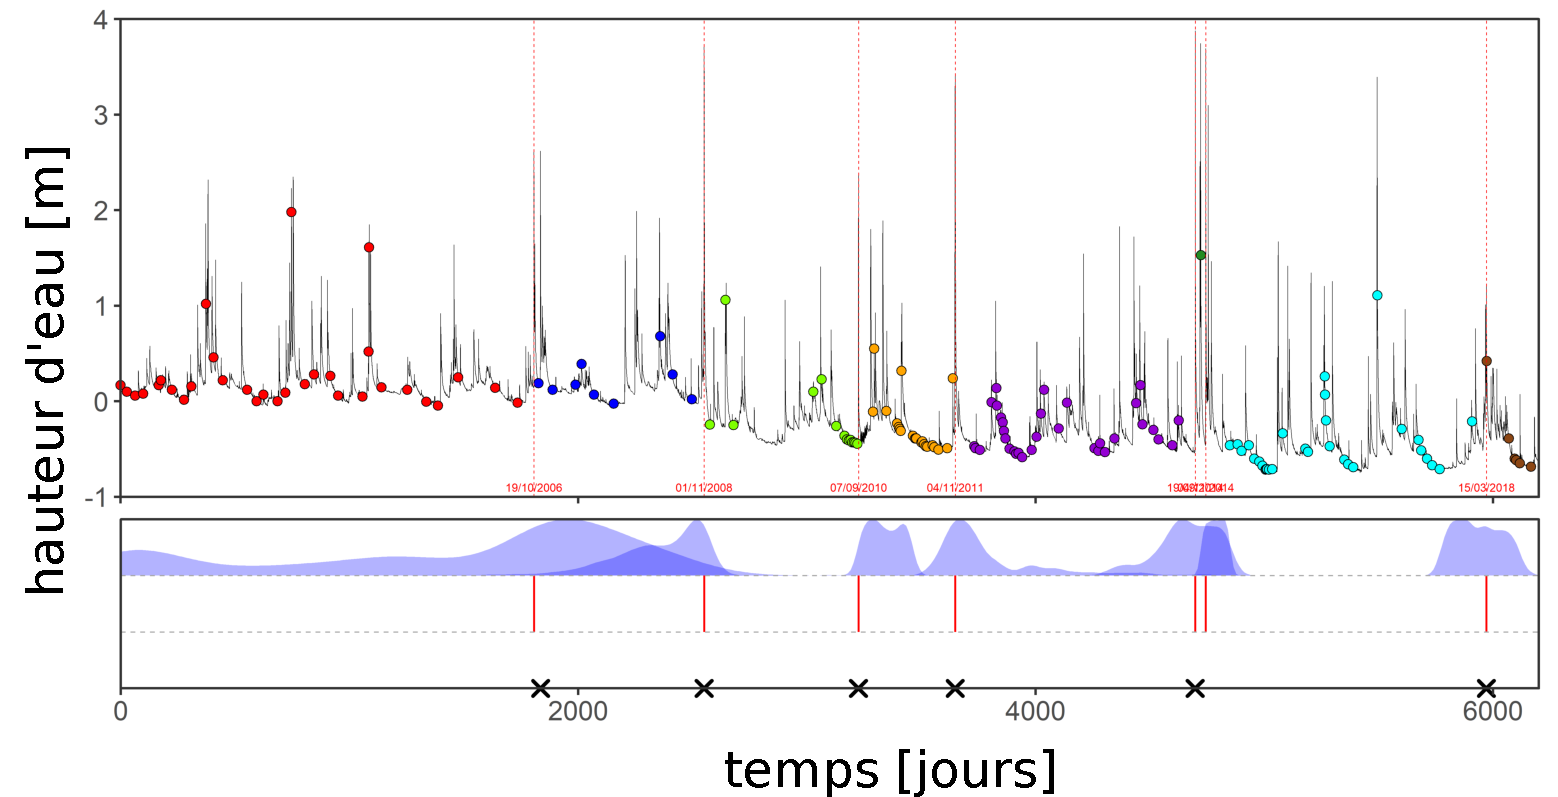
\includegraphics[width = .7\textwidth]{./Figures/Matt.pdf}
			\vfill
			\centering
			\begin{itemize}
				\item[$\vartriangleright$] Incertitude sur les dates de détarage $\rightarrow$ choix utilisateur
			\end{itemize}
		\end{center}
	\end{frame}
	
	  \begin{frame}
    		\frametitle{Estimation et propagation des incertitudes hydrométriques}
    		Comment estimer et propager l'ensemble des incertitudes hydrométriques ?
    		\vspace{15pt}
    		\begin{center}
    		\includegraphics<1>[width = .6\textwidth]{./Figures/HistoFloods1.pdf} 
      		\includegraphics<2>[width = .44\textwidth]{./Figures/SchemaProp1.pdf} 
			\includegraphics<3>[width = .44\textwidth]{./Figures/SchemaProp2.pdf} 
			\includegraphics<4>[width = .44\textwidth]{./Figures/SchemaProp3.pdf} 
%			\includegraphics<4>[width = .44\textwidth]{./Figures/SchemaProp0.pdf} 	
	     \end{center}
    \end{frame}
    
    \subsection{Courbes de tarage}
	\begin{frame}[t]
		\frametitle{Détermination des \textit{a priori}}
		\vfill
		\centering
		Nombreuses cartes et profils en travers dès 1845
		\begin{center}
			\includegraphics<1>[width = .6\textwidth]{./Figures/BathyPt.pdf} 
			\includegraphics<2>[width = .8\textwidth]{./Figures/EditArmand.pdf} 
			\includegraphics<3>[width = .8\textwidth]{./Figures/Goux4550.png} 
			\includegraphics<4>[width = .6\textwidth]{./Figures/ProfilsBardRestit.png} 
		\end{center}	
	\end{frame}    
	
%	\subsubsection{CT multi}	
	%%%%%%%%% X %%%%%%%%%
    \begin{frame}
    Modèle de courbes de tarage multipériodes : \textbf{BaRatin SPD} (Stage-Period-Discharge)\footfullcite{mansanarez_shift_2019}
    \vfill
    	\frametitle{Estimation des courbes de tarage}
		\begin{minipage}{.44\textwidth}
		\begin{itemize}
			\item<1->[$\vartriangleright$] Périodes avec peu/pas de jaugeages
			\vspace{0.5cm}
			\item<2->[$\vartriangleright$] Paramètres constants entre périodes ? $\Rightarrow$ expertise terrain
			\vspace{0.5cm}
			\item<3->[$\vartriangleright$] Transfert d'informations entre périodes
			\vspace{0.5cm}
			\item<4->[$\vartriangleright$] Pas de "recyclage"
			\end{itemize}
		\end{minipage}
		\begin{minipage}{.55\textwidth}
			\begin{center}
				\includegraphics<3->[width = \textwidth]{./Figures/Spd.jpg} 	
			\end{center}
		\end{minipage}    	   	
    \end{frame}
    	
    		\begin{frame}
		\frametitle{Témoignages de crues (1500-2000)}
		\centering 
		\vfill
		Évolution temporelle des enjeux en lit mineur ? 
		\vfill
		\includegraphics[width = .8\textwidth]{./Figures/Nb_C3-C4.pdf}
	\end{frame}

	
	

\end{document}

